%% ----------------------------------------------------------------
%% Thesis.tex -- MAIN FILE (the one that you compile with LaTeX)
%% ---------------------------------------------------------------- 

% Set up the document

%\documentclass[a4paper, 12pt, oneside]{Thesis}  % Use the "Thesis" style, based on the ECS Thesis style by Steve Gunn
\documentclass[a4paper, 12pt, twoside, openright]{Thesis} % use this for printing - or only use 'book' in document class


%\graphicspath{Figures/}  % Location of the graphics files (set up for graphics to be in PDF format)

% Include any extra LaTeX packages required
\usepackage[square, numbers, comma, sort&compress]{natbib}  % Use the "Natbib" style for the references in the Bibliography
\usepackage{verbatim}  % Needed for the "comment" environment to make LaTeX comments
\usepackage{vector}  % Allows "\bvec{}" and "\buvec{}" for "blackboard" style bold vectors in maths
\hypersetup{urlcolor=blue, colorlinks=true}  % Colours hyperlinks in blue, but this can be distracting if there are many links.

% new added by me. Faraz
\usepackage{csquotes}
\usepackage{multirow}


\usepackage{textcomp} % https://tex.stackexchange.com/a/58250/150467
\usepackage[table]{xcolor}
%\definecolor{cyan}{RGB}{0,255,255}
\definecolor{violet}{RGB}{143,0,255}
\definecolor{lightgray}{RGB}{235,235,235}
\definecolor{cream}{RGB}{247,245,213}
\definecolor{darkbrown}{RGB}{133,101,15}
\definecolor{pgreen}{rgb}{0,0.5,0}
\definecolor{somedarkcolor}{RGB}{200,0,100}
\usepackage{enumerate}% http://ctan.org/pkg/enumerate (added 20th nov, 2017)

\newcommand{\fanew}[1]{\textcolor{somedarkcolor}{#1}}
%Later:
%\newcommand{\fanew}[1]{#1}



\newcommand{\highlight}[1]{{\setlength\fboxsep{1pt}\colorbox{cream}{#1}}} % https://tex.stackexchange.com/a/88979/150467

\usepackage{mdframed} % https://tex.stackexchange.com/a/36528/150467
\mdfdefinestyle{MyFrame}{%
	linecolor=black,
%	outerlinewidth=2pt,
%	roundcorner=20pt,
	innertopmargin=\baselineskip,
	innerbottommargin=\baselineskip,
%	innerrightmargin=20pt,
%	innerleftmargin=20pt,
%	backgroundcolor=gray!50!white
}

% to avoid underlined text going out of page margins use \ul of the soul package
\usepackage{soul} % https://tex.stackexchange.com/a/9552/150467


\usepackage{emptypage} % to remove headers on empty pages inserted between chapters to start new chapter on odd page/right side
\usepackage{float} % so tables don't appear where they like, but order in they appear in code
\usepackage{tabularx} % so tables don't become too wide and exceed margin
\usepackage{footnote}
\usepackage{threeparttable}

\usepackage{subfig}

%%%% works with xelatex <START>
%%%% comment following lines related to fonts... and set compilation engine to pdflatex and build to get the title page with logos
%%%% uncomment the following lines and compile with xelatex to get correct non-english languages rendered in the thesis
%%%% compilation engine should be set to xelatex finally; so urdu, arabic, chinese texts get correctly rendered...

\usepackage{xeCJK}
\setCJKmainfont{Microsoft JhengHei} % MingLiU   Microsoft JhengHei

\usepackage{fontspec}

\usepackage{polyglossia}
\setmainlanguage{english}
\setotherlanguage{urdu}
\newfontfamily\urdufont[Script=Arabic]{Mehr Nastaliq Web}

\setotherlanguage{arabic}
\newfontfamily\arabicfont[Script=Arabic,Scale=1.5]{Traditional Arabic}

%%%% works with xelatex <END>

\newcommand{\qq}{\symbol{34}} % 34 is the decimal ascii code for "

\usepackage{listings, lstautogobble} % https://tex.stackexchange.com/a/162360/150467
\lstset{
	basicstyle=\ttfamily,
	language = C++,
	commentstyle=\color{pgreen},
	columns=flexible,
	breaklines=true,
	frame=single,
	autogobble=true,
	showspaces=true,
}
\usepackage{lstlinebgrd} % https://tex.stackexchange.com/a/331843/150467

\usepackage{siunitx} % https://tex.stackexchange.com/a/6105/150467
%% ----------------------------------------------------------------
\begin{document}
\frontmatter      % Begin Roman style (i, ii, iii, iv...) page numbering


\thispagestyle{empty}
{%%%
	\sffamily
	\centering
	\Large
	
	\vspace{\fill}
	
	%\setlength{\parskip}{0pt}
	{\LARGE Saarland University \\}
	{\Large Max Planck Institute for Informatics \\}
	\bigskip
	\bigskip
	\bigskip
	{\huge \bf \textbf{Improved Multilingual Temporal Tagging with HeidelTime} \\}
	\bigskip
	\bigskip
	{Master's Thesis in Computer Science \\}
	{by \\}
	{\LARGE Faraz Ahmad \\}
	\bigskip
	\bigskip
	{supervised and advised by \\}
	{\LARGE Dr. Jannik Str{\"{o}}tgen \\}
	\bigskip
	\bigskip
	\bigskip
	{reviewers \\}
	{\LARGE Dr. Jannik Str{\"{o}}tgen \\}
	{\LARGE Prof. Dr. Gerhard Weikum \\}
	\bigskip
	\bigskip
	{\Large May 9, 2018 \\}
	\bigskip
	\bigskip
	\bigskip
	\bigskip
	
%	\begin{figure}[h]
%		\centering
%		\subfloat{\includegraphics[height=2.2cm]{university}}
%		\hfill
%		\subfloat{\includegraphics[height=1.8cm]{mpi-inf}}
%	\end{figure}

\begin{figure}[h]
	\centering
	\subfloat{\includegraphics[height=2.2cm]{university}}
	\hfill
	\subfloat{\includegraphics[height=1.8cm]{mpi-inf}}
\end{figure}
	
	
	\vspace{\fill}
	
	
	%%%
}%%%
%% ----------------------------------------------------------------

\setstretch{1.3}  % It is better to have smaller font and larger line spacing than the other way round

% Define the page headers using the FancyHdr package and set up for one-sided printing
\fancyhead{}  % Clears all page headers and footers
\rhead{\thepage}  % Sets the right side header to show the page number
\lhead{}  % Clears the left side page header
\pagestyle{fancy}  % Finally, use the "fancy" page style to implement the FancyHdr headers

\cleardoublepage

%% ----------------------------------------------------------------
% Declaration Page required for the Thesis, your institution may give you a different text to place here
\thispagestyle{empty}
\Declaration{

%\addtocontents{toc}{\vspace{1em}}  % Add a gap in the Contents, for aesthetics

\textbf{Erklärung}\\
Ich erkläre hiermit, dass ich die vorliegende Arbeit selbständig verfasst und keine anderen als die angegebenen Quellen und Hilfsmittel verwendet habe. \\


\textbf{Statement}\\
I hereby confirm that I have written this thesis on my own and that I have not used any other media or materials than the ones referred to in this thesis.

\bigskip
\bigskip
\bigskip
\bigskip
\bigskip
 
\textbf{Einverständniserklärung}\\
Ich bin damit einverstanden, dass meine (bestandene) Arbeit in beiden Versionen in die Bibliothek der Informatik aufgenommen und damit veröffentlicht wird.\\

\textbf{Declaration of Consent}\\
I agree to make both versions of my thesis (with a passing grade) accessible to the public by having them added to the library of the Computer Science Department. 

\bigskip
\bigskip
\bigskip
\bigskip
\begin{table}[H]

\begin{tabularx}{\linewidth}{ X r }
	Saarbrücken, \underline{\hspace{5cm}} & \underline{\hspace{5cm}} \\ 
	\hspace{3.5cm}(Datum/Date) & (Unterschrift/Signature)\hspace{.2cm}
\end{tabularx}
\end{table}

%Saarbrücken, \underline{\hspace{3cm}}

%\rule[1em]{25em}{0.5pt}  % This prints a line to write the date

%\hfill

%(Faraz Ahmad) \underline{\hspace{3cm}}\\
%\rule[1em]{25em}{0.5pt}  % This prints a line for the signature

}

\clearpage  % Declaration ended, now start a new page

\cleardoublepage

%% ----------------------------------------------------------------
%% The "Funny Quote Page"
%\pagestyle{empty}  % No headers or footers for the following pages
%\null\vfill
%%% Now comes the "Funny Quote", written in italics
%\textit{``Write a funny quote here.''}
%
%\begin{flushright}
%If the quote is taken from someone, their name goes here
%\end{flushright}
%
%\vfill\vfill\vfill\vfill\vfill\vfill\null
%\clearpage  % Funny Quote page ended, start a new page
%% ----------------------------------------------------------------

% The Abstract Page
\addtotoc{Abstract}  % Add the "Abstract" page entry to the Contents
\abstract{
\addtocontents{toc}{\vspace{1em}}  % Add a gap in the Contents, for aesthetics

One important sub-task of information extraction is that of temporal tagging. Temporal tagging is a two step process that consists of extracting the temporal expressions and normalizing them to a standard ISO date format. This is an important task because temporal information can be utlilised to make robust question answering systems, enrich knowledge bases with temporal information, return better search results that are time-aware, among others. One multilingual and domain-sensitive temporal tagger that is available freely is HeidelTime. It is a rule-based tagger that can tag documents in 13 languages using manually developed resources by language experts; in addition to that, it can also tag documents in over 200 languages using automatically developed resources. It can also tag documents in various domains such as news or narrative type documents.

In this thesis, we extend the current HeidelTime multilingual model to create better automatically devloped resources for over 200 languages, so that the baseline tagging performance of HeidelTime for these, more than 200, languages can be improved. We extend the model in three ways: 1) We improve the automatically developed resources for the morphologically rich languages such as Finnish, Estonian, etc. 2) We improve the automatically developed resources for unsegmented languages such as Chinese and Japanese. 3) We improve the automatically developed resources generally for all the languages by enriching language-independent rules with new language-dependent rules that are learned from frequently occurring temporal patterns in respective languages. Finally, we present our results of running several evaluations and experiments using available temporally annotated corpora and Wikipedia dumps for various languages, and summarize our findings. 
}

\clearpage  % Abstract ended, start a new page
\cleardoublepage

%% ----------------------------------------------------------------

\setstretch{1.3}  % Reset the line-spacing to 1.3 for body text (if it has changed)

% The Acknowledgements page, for thanking everyone
\acknowledgements{
\addtocontents{toc}{\vspace{1em}}  % Add a gap in the Contents, for aesthetics
\hfill \textarabic{الحمد لله حمداََ کثیراََ طیباََ ...}\\

I would like to thank my thesis advisor Dr. Jannik Strötgen for giving me the opportunity to work under his supervision, for his valuable feedback and advice, and answering all my queries throughout the thesis. 

I would also like to thank Prabal Agarwal and Muhammad Ali for their valuable suggestions and feedback regarding the thesis.

I would also like to thank IMPRS-CS (International Max Planck Research School for Computer Science) for their assistance and financial support.

I would also like to thank all my friends at Saarbrücken for their friendship, help and time. 

I would also like to thank all my teachers, lecturers and professors for their their guidance. 

I would also like thank to my parents and my siblings for their love, support and prayers. 

Finally, I would like to thank all who rendered their support and/or made dua for me.

}
\clearpage  % End of the Acknowledgements
\cleardoublepage
%% ----------------------------------------------------------------

\pagestyle{fancy}  %The page style headers have been "empty" all this time, now use the "fancy" headers as defined before to bring them back

%% ----------------------------------------------------------------
\lhead{\emph{Contents}}  % Set the left side page header to "Contents"
\tableofcontents  % Write out the Table of Contents

%% ----------------------------------------------------------------
\lhead{\emph{List of Figures}}  % Set the left side page header to "List if Figures"
\listoffigures  % Write out the List of Figures

%% ----------------------------------------------------------------
\lhead{\emph{List of Tables}}  % Set the left side page header to "List of Tables"
\listoftables  % Write out the List of Tables

%% ----------------------------------------------------------------
%\lhead{\emph{List of Listings}}  % Set the left side page header to "List of Tables"
%\lstlistoflistings  % Write out the List of Tables

%% ----------------------------------------------------------------
% \setstretch{1.5}  % Set the line spacing to 1.5, this makes the following tables easier to read
% \clearpage  % Start a new page
% \lhead{\emph{Abbreviations}}  % Set the left side page header to "Abbreviations"
% \listofsymbols{ll}  % Include a list of Abbreviations (a table of two columns)
% {
% \textbf{Acronym} & \textbf{W}hat (it) \textbf{S}tands \textbf{F}or \\
% \textbf{LAH} & \textbf{L}ist \textbf{A}bbreviations \textbf{H}ere \\
%}

%% ----------------------------------------------------------------

% \clearpage  % Start a new page
% \lhead{\emph{Physical Constants}}  % Set the left side page header to "Physical Constants"
% \listofconstants{lrcl}  % Include a list of Physical Constants (a four column table)
% {
% % Constant Name & Symbol & = & Constant Value (with units) \\
% Speed of Light & $c$ & $=$ & $2.997\ 924\ 58\times10^{8}\ \mbox{ms}^{-\mbox{s}}$ (exact)\\
% }


%% ----------------------------------------------------------------

% \clearpage  %Start a new page
% \lhead{\emph{Symbols}}  % Set the left side page header to "Symbols"
% \listofnomenclature{lll}  % Include a list of Symbols (a three column table)
% {
% % symbol & name & unit \\
% $a$ & distance & m \\
% $P$ & power & W (Js$^{-1}$) \\
% & & \\ % Gap to separate the Roman symbols from the Greek
% $\omega$ & angular frequency & rads$^{-1}$ \\
% }


%% ----------------------------------------------------------------
% End of the pre-able, contents and lists of things
% Begin the Dedication page

\setstretch{1.3}  % Return the line spacing back to 1.3
\thispagestyle{empty}
\pagestyle{empty}  % Page style needs to be empty for this page
\dedicatory{To my parents and my siblings}

\addtocontents{toc}{\vspace{1em}}  % Add a gap in the Contents, for aesthetics


%% ----------------------------------------------------------------
\mainmatter	  % Begin normal, numeric (1,2,3...) page numbering
\pagestyle{fancy}  % Return the page headers back to the "fancy" style

\fancyhf{}
\fancyhead[lo]{\slshape\nouppercase{\rightmark}}
\fancyhead[re]{\slshape\nouppercase{\leftmark}}
%\fancyhead[ro,le]{\thepage}
\cfoot{\thepage}

% Include the chapters of the thesis, as separate files
% Just uncomment the lines as you write the chapters

\chapter{Introduction} \label{the-chapter-1}
\section{Motivation}
In most Information Extraction tasks, the first step is that of Named Entity Recognition \cite{DBLP:books/lib/JurafskyM09}. It deals with the extraction of named entities, such as names of persons, locations and organizations. The named entities occur frequently with events and time references, especially in documents belonging to the news domain. The terms in text that refer to absolute points in time, relative times or durations are called temporal expressions \cite{DBLP:books/lib/JurafskyM09}. The extraction of temporal expressions and events, in addition to the extraction of named entities can enable us to extract relations between entities and events to make information extraction more rich temporally. For instance, in the text ``Saarland University was established in 1948.", if temporal expression ``1948" is extracted, in addition to the entity ``Saarland Universiy" and the relation ``established"; this fact can be learned.

Temporal tagging is one of the sub tasks of Information Extraction; and has two steps, i.e., extraction and normalization of temporal expressions. The original focus of temporal tagging was news domain in its beginning \cite{DBLP:series/synthesis/2016Strotgen}, and most research has focused on processing English text documents till most recently \cite{DBLP:phd/de/Strotgen15}. Temporal tagging can be of great use in this age of smart-phones and influx of data; some potential application areas which can benefit from temporal tagging are:

\begin{itemize}
	\item \textbf{Information Retrieval:} One way to improve information retrieval for temporal needs is to take into account the temporal content in documents for ranking; for instance, Tiwiki \cite{DBLP:conf/www/AgarwalS17} is one such time-aware search engine for Wikipedia.  
	\item \textbf{Information Extraction:} Knowledge bases such as YAGO2 \cite{DBLP:journals/ai/HoffartSBW13} can benefit by extracting temporal scope with facts that have them; for instance, ``Jacques Chirac'' \texttt{holdsPoliticalPosition} ``President of France'' with temporal scope 1995-2007 \cite{DBLP:conf/www/KuzeyW12}. 
	\item \textbf{Personal Assistants:} In recent years, many personal assistants, such as Siri\footnote{\url{https://www.apple.com/ios/siri/}}, Cortana\footnote{\url{https://www.microsoft.com/en-us/windows/cortana}} and Alexa\footnote{\url{https://www.amazon.com/meet-alexa/b?ie=UTF8&node=16067214011}} have emerged on the scene to help users to search web, set reminders and manage calenders. These assistants can be synced to personal calender and email, that allows them to extract out events such as meeting reminders or a package delivery date from emails and add them to calender of user automatically. Many of these personal assistants are regularly updated to support further languages, in addition to English.
\end{itemize}

As mentioned earlier, until recently, most of the research on temporal tagging focuses on English language or a handful of other languages. The usual approaches of porting taggers from one language to another were difficult and often resulted in lower tagging quality \cite{DBLP:phd/de/Strotgen15}. HeidelTime\footnote{\url{https://github.com/HeidelTime/heideltime}} is a publicly available temporal tagger that has strict separation between algorithmic part and resources, that allows for easy adding of new modules to extend it for more languages \cite{DBLP:phd/de/Strotgen15}. At present, as of version 2.2.1, researchers have made available manual resources for 13 languages, such as Arabic \cite{strotgen2014time}, Croatian \cite{skukan2014heideltime} and French \cite{moriceau2013french}. Furthermore, Str{\"{o}}tgen and Gertz  in \cite{DBLP:conf/emnlp/StrotgenG15} made automatically developed resources for over 200 languages. 

The automatically developed resources of HeidelTime have shown promising results. For instance, on FR-TimeBank, a French temporal corpus, the F1 score for extraction phase using automatically developed resources was 70.8 compared to 91.0 when using the manually developed resources; the F1 score for normalization phase using automatically developed resources was 54.6 versus 73.6 when using the manually developed resources \cite{DBLP:conf/emnlp/StrotgenG15}. However, it was further shown in \cite{DBLP:conf/emnlp/StrotgenG15}, that the recall for couple of the languages evaluated using these automatically developed resources was lower in general. 

As mentioned earlier, HeidelTime has automatically developed resources for over 200 languages. These automatically developed resources can be used as baseline to tag documents temporally in over 200 languages; furthermore, these resources can also act as a starting point to extend them into manual ones \cite{DBLP:conf/emnlp/StrotgenG15}. Our goal, in this thesis is to improve the baseline quality of tagging using the automatically developed resources. To achieve our goal, we have identified three areas to improve automatically developed resources in: i) make them better for morphologically rich languages. ii) make them better for unsegmented languages. iii) make them better in general by learning frequently occurring temporal expressions as language-specific rules.  Furthermore, we aim to do detailed analysis using various corpora and Wikipedia dumps\footnote{\url{https://dumps.wikimedia.org/}}.

\section{Problem Statement}
While temporal tagging is an active research problem for English, very few systems have support for many languages. HeidelTime is a truly multilingual temporal tagger that supports over 200 languages using the automatically developed resources. Str{\"{o}}tgen and Gertz in \cite{DBLP:conf/emnlp/StrotgenG15} explain how the automatically developed resources were realized for HeidelTime. These automatically developed resources, while providing baseline temporal tagger for many languages for the first time, have following shortcomings:
\begin{itemize}
	\item \textbf{Disregards inflection:} A major issue with automatically developed resources of HeidelTime is that the morphological changes of words, i.e., inflections, are not covered.
	\item \textbf{Ignores unsegmented languages:} The automatically developed resources have same rules for all languages and these rules use a space to join individual patterns in rules. As unsegmented languages do not use space as delimeter, so automatically developed resources perform poorly on such languages. 
	\item \textbf{No language-specific rules:} The automatically developed resources, as they use same rules for all languages, ignore the intricacies of different languages and how temporal expressions might appear in them. 
	\item \textbf{Evaluating languages that lacked corpora:} The authors in \cite{DBLP:conf/emnlp/StrotgenG15} evaluated automatically developed resources for languages that had temporally annotated corpora available, it is obviously hard to evaluate the languages that have no corpora available. 
\end{itemize}

\section{Contributions}
The contribution of this thesis is creation of new automatically developed resources for HeidelTime, making the following improvements to the previous version:
\begin{itemize}
	\item We enhance the automatically developed resources to accommodate morphologically rich languages.
	\item We adjust the automatically developed resources to accommodate unsegmented languages.
	\item We enhance the automatically developed resources for all languages by learning frequently occurring temporal language specific temporal patterns as rules.
	\item We run detailed evaluations and analysis, i.e., evaluations on available temporally annotated corpora and analysis using Wikipedia dumps for other languages.
\end{itemize}
\section{Outline}
The remainder of this thesis is organized as follows: In Chapter \ref{the-chapter-2}, we explain some basic concepts and discuss the related work. In Chapter \ref{the-chapter-3}, we discuss the HeidelTime and its multilingual model. In Chapter \ref{the-chapter-4}, we describe our implementation of improved HeidelTime multilingual  model. In Chapter \ref{the-chapter-5}, we present in detail the evaluations and our findings. Finally, in Chapter \ref{the-chapter-6}, we give conclusion and list future directions. % Introduction

\chapter{Basic Concepts and Related Approaches} \label{the-chapter-2}
\section{Multilingual Natural Language Processing}
Natural language processing (NLP) aims to get computers to perform useful tasks that involve human language \cite{DBLP:books/lib/JurafskyM09}. The systems that incorporate NLP include machine translation systems, message-understanding systems, text-to-speech synthesis systems, speech recognition systems, multilingual information retrieval, among others; in general, any system that does useful speech or text processing.

Among above mentioned systems that require Multilingual NLP are machine translation systems and multilingual information retrieval systems; in both these systems multilingual natural language processing is required and pose a major challenge. Conferences such as MUC have played a major role in invigorating research in NLP, and also in multilingual NLP. For instance, multilingual named entities recognition evaluation was run using training and test article from comparable domains for all languages in MUC-7 conference \cite{chinchor1998overview}. 



\section{Temporal Information}
Documents contain implicit and explicit temporal information that can be utilized; the temporal information in documents can occur in many forms that include temporal expressions in documents, document creation time and document focus time \cite{DBLP:journals/ftir/KanhabuaBN15}. Document creation time (DCT) is one simple kind of temporal information which is almost occurs with all textual documents. Temporal information can also occur in user queries; for instance, in seasonal queries like ``black friday deals" or ``new iphone" \cite{DBLP:conf/sigir/Shokouhi11}. To capture the temporal information occurring in documents, one can use offsets or some custom tags. However, special annotation schemes have also been developed for consistency and interoperability. 

\subsection{Temporal Expressions} \label{sec_temp_ex}
Temporal expressions, as defined by Schilder and Habel in \cite{DBLP:conf/ndqa/SchilderH03}, refer to chunks of text that represent some sort of direct or inferred temporal information. In general, temporal expressions can be classified into explicit, implict and relative types \cite{DBLP:conf/ndqa/SchilderH03, DBLP:journals/sigir/AlonsoGB07}. 
\begin{enumerate}[i.]
	\item Explicit temporal expressions are such that can be easily normalized to exact time point on the Gregorian calendar; for example, `22 December 1997'.
	\item Implicit temporal expressions are such that need additional comprehension to normalize to exact time point; for example, `Mother's Day 2003'.
	\item Relative temporal expressions are such that need a reference time relative to which they must be normalized; for example, `last week' needs document creation time or some reference in text to normalize correctly.
\end{enumerate}

In addition to the above mentioned temporal expression types, Str{\"{o}}tgen and Gertz in \cite{DBLP:series/synthesis/2016Strotgen} define another type, i.e., underspecified temporal expressions. This type is closest to the relative type in the above three types, nevertheless, distinct. The difference is that in underspecified temporal expression we need to find the expression's `relation' to the reference time, in addition to finding the reference time itself, to correctly normalize it. The example we gave above for relative was `last week'; we only need to find the reference time in such case to correctly normalize it as the `last' word defines the relation to the reference time, i.e., the week before. However, to normalize a temporal expression such as `December', we need to find whether this December occurs before or after the reference time, in addition to finding the reference time itself, so `December' is an underspecified temporal expression. This also illustrates the difficulty of normalizing temporal expressions to correct values. 

\subsection{Annotation Schemes} \label{ss2as}
Temporal information can be extracted and annotated by enclosing temporal expressions in special tags, noting their offset positions in the document or in any desired way. However, it makes sense to have a common annotation standard that aids research. Two current annotation schemes being used by the research community are TIDES TIMEX2 standard by Ferro et al. in \cite{ferro2001tides, ferro2005tides} and TimeML Specification Language by Pustejovsky et al. in \cite{DBLP:journals/lre/PustejovskyKLS05, DBLP:conf/ndqa/PustejovskyCISGSKR03}. Both the standards use XML tags (TIDES uses TIMEX2, TimeML uses TIMEX3) with some properties; one such property is VALUE that represents the normalized value of the respective temporal expression in ISO8601 standard \cite{iso86012000data}. Some standard ISO8601 patterns and sample values are given in the table below (for details see \cite{iso86012000data}):

\begin{table}[H]
	\centering
	\rowcolors{1}{}{cream}
	\begin{threeparttable}
	\begin{tabular}{||l l l||} 
		\hline
		\textbf{Temporal Unit} & \textbf{Pattern} & \textbf{Sample Value} \\ [0.5ex] 
		\hline\hline
		complete calendar date & YYYY-MM-DD\tnote{1} & 1999-12-23 \\ 
		specific month & YYYY-MM & 1978-01 \\
		specific year & YYYY & 1978 \\
		specifc century & YY & 21 \\
		complete week date & YYYY-Www-D\tnote{2} & 2011-W02-7\\
		specific week & YYYY-Www\tnote{3} & 2011-W02 \\
		24 hour clock time & HH:MM:SS\tnote{4} & 23:59:59 \\
		complete date and time & YYYY-MM-DDThh:mm:ss\tnote{5} & 1985-04-22T12:16:30 \\
		incomplete date and time & YYYY-MM-DDThh:mm & 1985-04-22T12:16 \\
		complete duration & PYYYY-MM-DDThh:mm:ss & P0002-10-15T10:30:20 \\
		complete duration\tnote{6} & Pn\underline{n}Yn\underline{n}Mn\underline{n}DTn\underline{n}Hn\underline{n}Mn\underline{n}S & P0002-10-15T10:30:20\tnote{7} \\		
		\hline
	\end{tabular}
	\begin{tablenotes}
		\item[1] in extended format, it has - as separators for parts of dates \par and : as separators for parts of clock times,
		\item[2] D can be 1 for Monday up to 7 for Sunday,
		\item[3] ww represents number of calendar week within a year,
		\item[4] HH can be 24 only to represent end of a calendar day,
		\item[5] T character is used to indicate start of representation of time component,
		\item[6] format with designators, underlined n means zero or more digits.
		\item[7] a period/duration of 2 years, 10 months, 15 days, 10 hours, 30 minutes	and 20 seconds.
	\end{tablenotes}
	\end{threeparttable}
	\caption{Some sample date and time representations in ISO8601 standard.}
	\label{table:1a}
\end{table}

Now we explain the TimeML Specification Language with some examples. 

\textbf{TimeML}\\ 
TimeML is a modeling language specification which makes it easier to represent temporal expressions, temporal events and relationships between them \cite{DBLP:journals/lre/PustejovskyKLS05}. TimeML uses custom XML tags to capture temporal information. The four primary kinds of temporal tags as defined by TimeML are TIMEX3, EVENT, SIGNAL and LINK \cite{DBLP:conf/ndqa/PustejovskyCISGSKR03, pustejovsky2002annotation, ingria2002timeml}. The TIMEX3 tag captures the temporal expressions such as times, dates and durations. The EVENT tag is used to capture temporal events in text. The SIGNAL tag is used to capture temporal function words; for instance, ``before". Finally, the LINK tag is used to capture link between the aforementioned tags. 

The TIMEX3 tag is modeled on the original TIMEX tag by Setzer in \cite{DBLP:phd/ethos/Setzer01} and also on the TIDES TIMEX2 tag by Ferro et al. in \cite{ferro2001tides, ferro2005tides}. We illustrate the tasks of temporal expression extraction and temporal expression normalization using the following example:

\begin{mdframed}[style=MyFrame]
	\sloppy
	The \ul{1998} FIFA World Cup final was held on \ul{12 July 1998} at the Stade de France, Saint-Denis.
\end{mdframed}

The two temporal expressions in this example, underlined, need to be successfully extracted and normalized by the complete task of temporal tagging.  

The task of temporal expression extraction will just enclose the temporal expressions found in any annotation scheme, we use TimeML TIMEX3 tags in this example, as shown below:

\begin{mdframed}[style=MyFrame]
	\sloppy
	The <TIMEX3>\ul{1998}</TIMEX3> FIFA World Cup final was held on <TIMEX3>\ul{12 July 1998}</TIMEX3> at the Stade de France, Saint-Denis.
\end{mdframed}

%\begin{lstlisting}
%The <TIMEX3>1998</TIMEX3> FIFA World Cup final was held on <TIMEX3>12 July 1998</TIMEX3> at the Stade de France, Saint-Denis.
%\end{lstlisting}

The task of temporal expression normalization will normalize the found temporal expressions to ISO dates format, using additional attributes of TIMEX3 tags in this example, as shown below:

\begin{mdframed}[style=MyFrame]
	\sloppy
	The <TIMEX3 tid=``t1" type=``DATE" value=``1998">\ul{1998}</TIMEX3> FIFA World Cup final was held on <TIMEX3 tid=``t4" type=``DATE" value=``1998-07-12">\ul{12 July 1998}</TIMEX3> at the Stade de France, Saint-Denis.
\end{mdframed}

In the above example, we see some of the attributes of TIMEX3 tags that aid in normalization, i.e., tid, type and value; tid is a unique id assigned to every TIMEX3 tag, type can be one of the following: TIME, DATE, DURATION or SET, value represents the normalized value of the temporal expression in ISO 8601 format. Each type captures a kind of temporal expression:

\begin{enumerate}[i.] \label{ss2as:timeml}
	\item Time temporal expressions are such that point to a time such that its granularity is less than that of a day. For instance, `The guests arrived at \ul{9 am}'.
	\item Date temporal expressions are such that point to a time such that its granularity is larger or equal to that of a day. For instance, `It was really cold in \ul{Fall 2003}'. 
	\item Duration temporal expressions are such that point to some length of time. For instance, `The family stayed for \ul{2 months}'.
	\item Set temporal expressions are such that point to some times which occur again and again. For instance, `He visited his family \ul{weekly}'.
\end{enumerate}
For more examples of TIMEX3 tags in use, see \cite{sauri2006timeml, timeml2009guidelines}.\\



\section{Temporal Taggers}
Temporal taggers are computer programs made for the purpose of automatic temporal tagging of documents, including both extraction and normalization of the temporal expressions in documents. As mentioned earlier, temporal tagging is a two step process, i.e., extraction and normalization. Therefore, the taggers need to perform both these tasks for the complete task of temporal tagging. Discussing two steps of temporal tagging is important here because in most taggers they are done separately with differing techniques. However, there are some tools available which only perform normalization; for example, TIMEN by Llorens et al. in \cite{DBLP:conf/lrec/LlorensDGS12}.




\subsection{Different Approaches for Tagging}
For the first task of temporal tagging, i.e., extraction, both rule-based and supervised machine-learning approaches are used. The rule-based approach makes use of regular expressions, pattern lists, part-of-speech information, among others \cite{DBLP:phd/de/Strotgen15}. The machine learning approaches used are supervised and need annotated corpora to learn patterns. 

For the second task of temporal tagging, i.e., normalization, rule-based approaches are used by almost all the taggers \cite{DBLP:phd/de/Strotgen15}, because of complex nature of the task. It is complex because it is difficult to normalize relative and under-specified expressions, especially in documents where document creation time is not available. 

The advantage of rule-based approaches is that the rules can be created without requiring temporally annotated corpora; thus, easy to extend to many languages. The disadvantage of rule-based approaches is that it requires manual effort, language experts and is time consuming to create the rules. On the other hand, machine learning approaches have the advantage of not requiring manual effort or language experts; but the disadvantage is that they require temporally annotated corpora. 

In the following table, we summarize some of the temporal taggers and approaches they use:

\begin{table}[H] \label{the-ttaggers-table1}
	\centering
	\rowcolors{1}{}{cream}
	\begin{threeparttable}
		\begin{tabular}{||l l l l||} 
			\hline
			\textbf{Temporal Tagger} & \textbf{Extraction} & \textbf{Normalization} & \textbf{Annotation} \\ [0.5ex] 
			\hline\hline
			TempEx \cite{DBLP:conf/acl/ManiW00} & rule-based & rule-based & TIMEX2 \\ 
			GUTime \cite{DBLP:conf/acl/VerhagenMSLKJRPP05} & rule-based & rule-based & TimeML \\
			Chronos \cite{negri2004recognition} & rule-based & rule-based & TIMEX2 \\
			TERSEO \cite{DBLP:journals/dke/SaqueteMM06} & rule-based & rule-based & TIMEX2 \\
			ATEL \cite{DBLP:conf/cicling/HaciogluCD05} & ML-based & - & TIMEX2 \\
			DANTE \cite{DBLP:conf/ltconf/MazurD07} & rule-based & rule-based & TIMEX2  \\
			TimexTag \cite{DBLP:conf/dagstuhl/AhnAR05, DBLP:conf/naacl/AhnRR07} & rule-based & rule-based & TIMEX2  \\
			TEA \cite{DBLP:conf/time/HanGL06} & rule-based & rule-based & TimeML  \\
			TIPSem \cite{DBLP:conf/semeval/LlorensSN10} & ML-based & rule-based & TimeML \\
			TIMEN \cite{DBLP:conf/lrec/LlorensDGS12}  & - & rule-based & TimeML  \\
			TRIPS/TRIOS \cite{DBLP:conf/semeval/UzZamanA10} & ML-based & rule-based & TimeML  \\
			SUTime \cite{DBLP:conf/lrec/ChangM12} & rule-based & rule-based & TimeML  \\
			UWTime \cite{DBLP:conf/acl/LeeADZ14} & hybrid\tnote{1} & hybrid\tnote{1} & TimeML \\
			HeidelTime \cite{DBLP:conf/semeval/StrotgenG10} & rule-based & rule-based & TimeML  \\ [1ex]
			\hline
		\end{tabular}
	\begin{tablenotes}
		\item[1] hybrid means it uses both rules and ML-techniques.
	\end{tablenotes}
	\end{threeparttable}
	\caption{Some of the temporal taggers and approaches they use.}
	\label{table:1b}
\end{table}



\subsection{Temporal Taggers for Non-English Corpora}
To invigorate the research in the area of temporal tagging, competitions such as ACE TERN and TempEval have been held in past years. With each subsequent version of these competitions, more languages were added in the competitions and researchers took part in these with temporal taggers for different languages. 

To process non-English languages, taggers can be classified into two types, i.e., specialized taggers or extensible taggers. The specialized taggers are made for a specific language from the get-go, while the extensible taggers are made with future extensibility to further languages in mind. One may further classify the latter type of taggers into two sub-types based on the amount of effort and knowledge about the tagger required to extend it to a new language \cite{DBLP:phd/de/Strotgen15}. 

An  example of a specialized tagger is TETI \cite{DBLP:conf/imcsit/CasellidP09} which tags Italian documents. An example of extensible tagger is Chronos \cite{negri2004recognition} which was developed for English originally and later extended to support Italian.

In the following table, we summarize some of the temporal taggers that can tag non-English corpora:  

\begin{table}[H] \label{the-ttaggers-table2}
	\centering
	\rowcolors{1}{}{cream}
	\begin{threeparttable}
		\begin{tabular}{||l l l||} 
			\hline
			\textbf{Temporal Tagger} & \textbf{Type} & \textbf{Language(s)} \\ [0.5ex] 
			\hline\hline
			Chronos \cite{negri2004recognition, negri2007dealing} & extensible & 2 (English, Italian)  \\
			TETI \cite{DBLP:conf/imcsit/CasellidP09} & specialized & 1 (Italian) \\
			TERSEO \cite{DBLP:journals/dke/SaqueteMM06, negri2006evaluating} & extensible & 3 (Spanish, English, Italian)  \\
			TIPSem \cite{DBLP:conf/semeval/LlorensSN10} & extensible & 4 (English, Spanish, Italian, Chinese)  \\
			HeidelTime \cite{DBLP:conf/semeval/StrotgenG10, DBLP:conf/emnlp/StrotgenG15} & extensible & 13 (and 200+)\tnote{1}   \\ [1ex]
			\hline
		\end{tabular}
		\begin{tablenotes}
			\item[1] HeidelTime has hand-crafted resources for 13 languages including English, German, Arabic, etc. also automatically developed resources for over 200 languages.
		\end{tablenotes}
	\end{threeparttable}
	\caption{Some temporal taggers that can tag non-English corpora.}
	\label{table:1c}
\end{table}



\subsection{Temporally Annotated Corpora} \label{tactac}
To compare the performance of different temporal taggers, researchers have made available some temporally annotated corpora, using either TIDES TIMEX2 or TimeML annotation scheme. Many of these corpora are for English language, such as ACE TERN 2004 Training, TimeBank v1.2 and TempEval-2. In recent years, corpora for other languages have also been made available, such as Arabic corpus of ACE 2005 Training, French TimeBank and Romanian TimeBank.

In the following table, we summarize some of the temporally annotated corpora available.
  
\begin{table}[H] \label{the-ttaggers-corpora-table}
	\centering
	\rowcolors{1}{}{cream}
	\begin{threeparttable}
		\begin{tabularx}{\linewidth}{||l   >{\raggedright\arraybackslash}X   >{\raggedright\arraybackslash}p{0.6in}   >{\raggedright\arraybackslash}p{1in}||} 
			\hline
			\textbf{Corpus} & \textbf{Language(s)} & \textbf{Scheme} & \textbf{Domain} \\ [0.5ex] 
			\hline\hline
			ACE 2005 \cite{walker2006ace} & Arabic, Chinese, English & TIMEX2 & news, blogs and discussion \\
%			ACE 2007 & Arabic, Spanish & TIMEX2 & news and blogs \\
			\hline
			TempEval-2 \cite{DBLP:conf/semeval/VerhagenSCP10} & Chinese, English, French, Italian, Korean, Spanish & TimeML & news \\
			TempEval-3 \cite{DBLP:conf/semeval/UzZamanLDAVP13} & English, Spanish & TimeML & news \\
			\hline
			AncientTimes \cite{DBLP:conf/lrec/StrotgenBZACG14}& Arabic, Dutch, English, French, German, Italian, Spanish, Vietnamese & TimeML & narratives \\
			\hline
			WikiWarsDE \cite{strotgen2011wikiwarsde} & German & TIMEX2 & narratives \\
			WikiWarsVN \cite{strotgen2014time} & Vietnamese & TimeML & narratives \\
			WikiWarsHR \cite{skukan2014heideltime} & Croatian & TimeML & narratives \\
			\hline
			FR-TimeBank \cite{bittar2011french} & French & TimeML & news \\
			PT-TimeBank \cite{Costa:Branco:2012c}  & Portuguese & TimeML & news \\
			RO-TimeBank \cite{foruascu2012romanian} & Romanian & TimeML & news \\
			Ita-TimeBank \cite{caselli2011annotating} & Italian & TimeML & news \\
%			\hline
%			TIDES Parallel  & Spanish & TIMEX2 & dialogs \\ [1ex]
			\hline
		\end{tabularx}
		%\begin{tablenotes}
		%	\item[1] a footnote text placeholder ... 
		%\end{tablenotes}
	\end{threeparttable}
	\caption{Some multilingual temporally annotated corpora available.}
	\label{table:1d}
\end{table}

\subsection{Automated Approaches to Tackle Multilinguality}
Temporal taggers are generally made for a certain language, and temporal taggers that are rule based can be usually extended to support further languages \cite{DBLP:series/synthesis/2016Strotgen}. The task of extending a temporal tagger to support new language by adding new rules is a laborious one and requires respective language expert(s). Also, if the rules are not separated out from the general tagging system itself, the task of extending it to support another language will become more complex; as now one need to understand the working of system itself to add new rules. To add support of a new language to a temporal tagger some early semiautomatic approaches have been suggested. Some such approaches are discussed below.

Saquete et al. in \cite{DBLP:conf/micai/SaqueteMM04} present a semiautomatic extension of TERSO, a monolingual temporal tagger for Spanish. They present a five stage approach. The first step is a translation unit that translates Spanish temporal expressions from the TERSEO knowledge base into the target languages. The second step is debugger unit that uses Google to remove spurious translations of the first step. The third step is a keyword unit that uses Wordnet (as the target language is English) to get synonyms for the expressions it receives from the second stage. The fourth step gets even further expressions by running the tagger on a corpus of target language. The fifth step assigns a resolution to each temporal expression and they are added to the TERSEO knowledge base. Finally, integration of the extension system with TERSEO is done. The autors evaluated the first two units of the mentioned pipeline. No evaluation was performed to evalaute the annotation performance on an English corpora directly, though. 

TERSEO was further automatically ported to support Italian in by Negri et al. in \cite{negri2006evaluating}. The authors presented three evaluation strategies, i.e., first by using online translators, second by using knowledge from annotated corpora and third by using combined approach. The results were encouraging as a baseline, but ofcourse not close to state-of-the-art systems for Italian. 

Most automatically porting approaches till recenty, were limited to a small number of languages, results for normalization were not so good and only corpora of news domain were evaluated \cite{DBLP:series/synthesis/2016Strotgen}. However, Str{\"{o}}tgen and Gertz in \cite{DBLP:conf/emnlp/StrotgenG15} added support for over 200 languages in HeidelTime using the resources that were automatically developed, had good baseline scores for normalization in addition to extraction and tagged documents in domains other than news too. As the main goal of this thesis is to make automatically developed resources of HeidelTime further better, HeidelTime and its model for creating automatically developed resources will be explained in detail in Chapter \ref{the-chapter-3}.

\section{Linguistic Background}
To do linguistic analysis of any natural language, the characters, words, and sentences in any document need to be clearly defined; and defining these units present different challenges based on the language being processed; the task is not trivial considering the wide range of human languages and writing systems \cite{indurkhya2010handbook}.

Linguistic properties of a language should be kept in mind when designing any NLP system for respective language. Some of linguistic properties of various natural languages are discussed in this section. 

\subsection{Morphologically-rich Languages} \label{morphologically-rich-languages-background}
Morpheme is a smallest meaningful unit of a language. Morphology is the study of the structure words in a language and their relation to other words, while syntax is the study of the structure of sentences in a language. In morphologically-rich languages, the role of morphology is much greater, and correspondingly the role of syntax smaller; for instance, Turkish \cite{dressler2003morphological}. 

\subsection{Inflections}
Inflection is a phenomenon that changes the morphology of words in a language. Another such phenomenon is called derivation. An affix can be either inflectional or derivational. 

One characteristic, among others, that distinguishes inflectional morphemes from derivational morphemes is that inflectional morphemes typically occur with all members of some large class of morphemes; for instance, the plural morpheme -s in English occurs with almost all countable nouns; while derivational morphemes tpyically occur with some members of some large class of morphemes; for instance, the morpheme -hood in Enlgish can occur with only few words such as knight (see link\footnote{\url{http://www-personal.umich.edu/~jlawler/Inflection.pdf}}).  

The inflectional morphology for English is relatively simpler, while the inflectional morphological possibilities for some other languages are more numerous \cite{indurkhya2010handbook}. The languages that have large number of inflections are called synthetic languages. Another aspect worth mentioning is that agglutination and fusion are forms of inflection, among others. 

The difference between agglutination and inflection is summarised in table below:


\begin{table}[H] \label{the-inflection-table}
	\centering
	\rowcolors{1}{}{cream}
	\begin{threeparttable}
		\begin{tabularx}{\linewidth}{||>{\raggedright\arraybackslash}p{.8in}| >{\raggedright\arraybackslash}X >{\raggedright\arraybackslash}X||} 
			\hline
			\textbf{} &
			\textbf{Agglutinative inflection} & \textbf{Fusional inflection} \\ [0.5ex] 
			\hline\hline
			\textbf{Definition} & inflection refers to one category & inflection can refer to many categories \\
			\textbf{Example language} & Turkish  & Latin \\
			\textbf{Example inflection}  & `-iz' in Turkish refers a plural subject & `-tis' in Latin\tnote{1} can refer to second person plural subject of verb in present tense, active voice \\ [1ex]
			\hline
		\end{tabularx}
		\begin{tablenotes}
			\item[1] \url{https://linguistics.stackexchange.com/a/9384} 
		\end{tablenotes}
	\end{threeparttable}
	\caption{Inflection types.}
	\label{table:1e}
\end{table}

As noted earlier, some languages have numerous possibilites for inflectional morphology. For instance, the plural form in German is denoted by various endings such as `-en', `-er', `-e' or `-n'; moreover, the suffixes `-en' or `-n' are also used to represent cases \cite{indurkhya2010handbook}. Grammar of some languages such as Finnish have even greater number of cases than German does; thus, leading to a lot of inflections. 

The following table depicts inflections for the Finnish word `Tammikuu', that is the month name `January' in Finnish. 

\begin{table}[H] \label{the-inflection-table-tammikuu}
	\centering
	\rowcolors{1}{}{cream}
	\begin{threeparttable}
		\begin{tabularx}{\linewidth}{||>{\raggedright\arraybackslash}p{1.5in}| >{\raggedright\arraybackslash}X >{\raggedright\arraybackslash}X||} 
			\hline
			\multicolumn{3}{|l|}{\textbf{Inflection of tammikuu\tnote{1}} } \\
			\hline\hline
			\textbf{} & \textbf{singular} & \textbf{plural} \\
			\textbf{nominative} & tammikuu  & tammikuut \\
			\textbf{accusative nom.} & tammikuu  & tammikuut \\
			\textbf{accusative gen.} & tammikuun  & tammikuut \\
			\textbf{genitive} & tammikuun  & tammikuiden, tammikuiden \\
			\textbf{partitive} & tammikuuta  & tammikuita \\
			\textbf{inessive} & tammikuussa  & tammikuissa \\
			\textbf{elative} & tammikuusta  & tammikuista \\
			\textbf{illative} & tammikuuhun  & tammikuihin \\
			\textbf{adessive} & tammikuulla  & tammikuilla \\
			\textbf{ablative} & tammikuulta  & tammikuilta \\
			\textbf{allative} & tammikuulle  & tammikuille \\
			\textbf{essive} & tammikuuna  & tammikuina \\
			\textbf{translative} & tammikuuksi  & tammikuiksi \\
			\textbf{instructive} & - & tammikuin \\
			\textbf{abessive} & tammikuutta  & tammikuitta \\
			\textbf{comitative} & -  & tammikuineen \\ [1ex]
			\hline
		\end{tabularx}
		\begin{tablenotes}
			\item[1] \url{https://en.wiktionary.org/wiki/tammikuu#Finnish}
		\end{tablenotes}
	\end{threeparttable}
	\caption{Inflections of the Finnish word Tammikuu (January).}
	\label{table:1f}
\end{table}

%\begin{figure}[H]
%	\centering
%	\includegraphics[width=12cm]{january-finnish}
%	\caption{Finnish translation for `January' depicting inflections in language}
%	\label{figure:2a}
%\end{figure}

\subsection{Unsegmented Languages}
Languages such as Chinese, Japanese and Thai are fundamentally different than space-delimited languages, in that they lack any spaces between words \cite{indurkhya2010handbook}. The words are not separated using spaces in these languages, and there are no clear indication of word boundaries.  % Background Theory 

\chapter{HeidelTime and Its Multilingual Model} \label{the-chapter-3}
In this chapter, we give an overview of HeidelTime, discuss the data model of multilingual HeidelTime as presented by Str\"{o}tgen and Gertz in \cite{DBLP:conf/emnlp/StrotgenG15} and	 discuss some of its shortcomings.

\section{HeidelTime Overview}
HeidelTime is the first multilingual and domain-sensitive temporal tagger for the full task of temporal tagging \cite{DBLP:series/synthesis/2016Strotgen}. It has manually developed resources for 13 languages, and automatically developed resources for over 200 languages \cite{DBLP:conf/emnlp/StrotgenG15}. It is domain-sensitive, as in it can tag documents of differing domains such as news, narratives, scientific and colloquial \cite{DBLP:series/synthesis/2016Strotgen}. The online demo of HeidelTime can be accessed here\footnote{\url{http://heideltime.ifi.uni-heidelberg.de/heideltime/}}.

HeidelTime has been shown to perform very good in various competitions and corpora. It had best evaluation results for full task of temporal tagging for English in TempEval-2 \cite{DBLP:conf/semeval/VerhagenSCP10}, for English and Spanish in TempEval-3 \cite{DBLP:conf/semeval/UzZamanLDAVP13} and for Italian in Evalita 2014 \cite{caselli2014eventi}. In addition to the mentioned competitions, HeidelTime has been evaluated on various temporal corpora in languages such as Arabic, German, Chinese, among others\footnote{\url{https://github.com/HeidelTime/heideltime/wiki/Evaluation-Results}}. 

\subsection{Architecture}
HeidelTime's system architecture makes strict separation between algorithmic part (source code) and the resources part (patterns, rules and normalization information) \cite{DBLP:phd/de/Strotgen15}. The algorithmic core is language independent and written in Java, while the resources part is language dependent and written in .txt files arranged into three directories. One of HeidelTime's component called resource-interpreter, automatically loads the language dependent resources for tagging in the respective language if the resources are made in the format defined in \cite{DBLP:phd/de/Strotgen15}. This clear separation between algorithmic part and resources part in design of HeidelTime makes the manual extension to other languages appealing, which is evident from it being extended to languages such as German \cite{DBLP:phd/de/Strotgen15}, French \cite{moriceau2013french} and Croatian \cite{skukan2014heideltime}. 

\subsection{Availability}
HeidelTime is available as a standalone version and as a UIMA (Unstructured Information Management Architecture) kit (download link\footnote{\url{https://github.com/HeidelTime/heideltime/releases}}). The standalone version can be used in simpler cases; for instance, if only tagging is desired. The UIMA version of HeidelTime can be used in more advanced cases; for instance, to reproduce evaluation results. Apache UIMA\footnote{\url{https://uima.apache.org/}} is a Java framework that enables applications to be decomposed into components and use such components in a pipeline fashion. UIMA also defines a format called CAS (Common Analysis Structure), and all components in the pipeline work on CAS objects. As HeidelTime requires text to be pre-annotated with some preprocessing steps such tokenization, sentence splitting and part-of-speech tagging; and UIMA framework supports the idea of components in a pipelined fashion, HeidelTime was developed as a UIMA analysis engine component \cite{DBLP:phd/de/Strotgen15}. 

Some components bundled with HeidelTime UIMA version include: TempEval-2 Reader, a \ul{UIMA collection reader}, reads TempEval-2 annotated corpora and creates a CAS object for each document \cite{DBLP:phd/de/Strotgen15}. Heideltime, available as a \ul{UIMA analysis engine}, tags the documents temporally using TIMEX3 tags \cite{DBLP:phd/de/Strotgen15}. TempEval-3 Writer, a \ul{UIMA CAS consumer}, outputs temporally tagged documents in a format that official TempEval-3 evaluation scripts can run on \cite{DBLP:phd/de/Strotgen15}. The components to do preprocessing tasks such as tokenization, sentence splitting and part-of-speech tagging are also available with the HeidelTime kit as UIMA analysis engine components, and should be run before running the HeidelTime analysis engine component. 

\subsection{Resources}
For each language, HeidelTime arranges the resources into three directories, i.e., pattern resources, normalization resources and rule resources \cite{DBLP:phd/de/Strotgen15}. These directories hold .txt files, that have patterns, normalization and rules in them respectively.  

\textbf{Pattern Resources}\\
The pattern resources hold regular expressions for various kinds of temporal expressions such as month names, weekday names, etc. These .txt pattern files hold one regular expression on each line for legibility. The HeidelTime resource interpreter reads a pattern file and makes complete regular expression for respective pattern file automatically \cite{DBLP:phd/de/Strotgen15}. For instance, one of the file in pattern directory is called ``reMonthName", and for English language this file will hold the regular expressions for month names in English, i.e., [Jj]anuary, [Ff]ebruary, and so on in it. Similarly, for Urdu language it will have the month names \texturdu{جنوری}, \texturdu{فروری}, \texturdu{مارچ} and so on in it. 

Following listing depicts a part of a reMonthName for French language. \\

%\begin{figure}[H]
%	\centering
%	\includegraphics[width=8cm]{fr-reMonthName}
%	\caption{reMonthName - a sample French pattern resource for HeidelTime}
%	\label{figure:3a}
%\end{figure}

\begin{minipage}{\linewidth}
\lstset{caption={reMonthName - a sample French pattern resource for HeidelTime.}, label={listing:3-fr-reMonthName},}
\begin{lstlisting}
// english: January, 01
[Jj]anvier
// english: February, 02
[Ff]évrier
// english: March, 03
[Mm]ars
// english: April, 04
[Aa]vril
// english: May, 05
// ...
\end{lstlisting}
\end{minipage}

\textbf{Normalization Resources}\\
The normalization resources hold the temporal expression regular expressions and their normalized expressions separated by a comma, like a key-value pair. Like pattern .txt files, the normalization .txt files also hold one normalization information on each line. The HeidelTime resource interpreter reads a normalization file and holds the normalization information, so it can be used to assign normalized values to extracted temporal expressions. For instance, the first line in ``normMonthName" resource file for English can be \framebox{``[Jj]anuary",``01"} and the first line for Urdu can be \framebox{``\texturdu{جنوری}",``01"}

Following listing depicts a part of a normMonthName for French language. \\


%\begin{figure}[H]
%	\centering
%	\includegraphics[width=8cm]{fr-normMonthName}
%	\caption{normMonthName - a sample French normalization resource for HeidelTime}
%	\label{figure:3b}
%\end{figure}

%\begin{lstlisting}[
%caption={normMonthName - a sample French normalization resource for HeidelTime}, label={listing:3-fr-normMonthName}
%identifierstyle=\oddtest,
%commentstyle=\oddtest,
%stringstyle=\oddtest,
%keywordstyle=\oddtest,
%linebackgroundcolor={\ifodd\value{lstnumber}\color{cream}\fi}
%]
%... alternating , rows, colors
%... zebra color effect 
%\end{lstlisting}

\begin{minipage}{\linewidth}
\lstset{caption={normMonthName - a sample French normalization resource for HeidelTime.}, label={listing:3-fr-normMonthName},}
\begin{lstlisting}
// english: January, 01
"[Jj]anvier","01"
// english: February, 02
"[Ff]évrier","02"
// english: March, 03
"[Mm]ars","03"
// english: April, 04
"[Aa]vril","04"
// english: May, 05
// ...
\end{lstlisting}
\end{minipage}




\textbf{Rule Resources}\\
The rule resources hold the rules that are used to extract and normalize the temporal expressions from the text \cite{DBLP:phd/de/Strotgen15}. The rules extraction part make use of the pattern resources, and rules normalization part make use of the normalization resources. Like pattern and normalization resources, the rules are also read by HeidelTime's resource interpreter and made use of by its algorithmic part. HeidelTime defines a well-defined rule syntax to be used in the rule resources \cite{DBLP:phd/de/Strotgen15}. 

Each HeidelTime rule should have three obligatory parts, i.e., RULENAME, EXTRACTION and NORM\_VALUE. The RULENAME is helpful for statistics purposes, EXTRACTION part is used for extraction and here the names of pattern resources can be used to describe the regular expression to match, and NORMALIZATION part is used for normalization and here the names of normalization resources can be used \cite{DBLP:phd/de/Strotgen15}. In addition, rules may use some other parts such as specifying part-of-speech type of the token to extract. 

%We illustrate the rule syntax using a simple rule below, and for details refer the reader to Section 3.5.4 of \cite{DBLP:phd/de/Strotgen15}.

%\begin{figure}[H]
%	\centering
%	\includegraphics[width=14cm]{daterules}
%	\caption{rules\_daterules - a sample rule resource for HeidelTime}
%	\label{figure:3c}
%\end{figure}

Following listing shows a part of language independent rules resource of HeidelTime, that has some date rules in it.  \\

\begin{minipage}{\linewidth}
\begin{lstlisting}[caption={rules\_daterules - a sample rule resource for HeidelTime.}, label={listing:3-daterules}]
// r3a: March 30, 2000
// r3b: March 30

RULENAME="date_r3a",EXTRACTION="%reMonthName %reDayNumber,? %reYear4Digit",NORM_VALUE="group(3)-%normMonthName(group(1))-%normDayNumber(group(2))"

RULENAME="date_r3b",EXTRACTION="%reMonthName %reDayNumber",NORM_VALUE="UNDEF-year-%normMonthName(group(1))-%normDayNumber(group(2))"
// ...
\end{lstlisting}
\end{minipage}


In Listing \ref{listing:3-daterules}, some of the date rules are given. For instance, the rule named ``date\_3a" can extract dates such as \framebox{March 30, 2000} or \framebox{February 10 2012}. This can be gathered from the extraction part of the rule. We can see that the extraction part of the rule uses the pattern resources, by appending \% in front of the pattern resource name. Writing \%reMonthName will get all the month name patterns from the reMonthName pattern resource of a respective language. Following \%reMonthName is a space, then \%reDayNumber that refers to all patterns of day numbers from 1-31, then there is an optional comma, and finally the pattern \%reYear4Digit. 

In normalization part of the rule ``date\_3a", we see the normalized value that should be assigned to the extracted temporal expression. The first thing to notice is group(3); in HeidelTime each pattern in the extraction part counts as a group()-function, in addition to the patterns specified in parenthesis \cite{DBLP:phd/de/Strotgen15}. So in the order the pattern resource names appear in extraction part of rule, we can learn that \%reMonthName can be referred to as group(1), \%reDayNumber can be referred to as group(2) and \%reYear4Digit can be referred to as group(3) in the normalization part of the rule. Furthermore we can see, the group(1) and group(2) are enclosed in respective normalization functions, because reMonthName and reDayNumber will require normalization, unlike reYear4Digit. Thus, the normalization part is normalizing the extracted date to the ISO format (Table \ref{table:1a} page \pageref{table:1a}).

For a detailed overview of HeidelTime's rule syntax, we refer the reader to Section 3.5.4 of \cite{DBLP:phd/de/Strotgen15}.

\section{Multilingual HeidelTime Model} \label{multilingual-ht-model}
HeidelTime was extended to support over 200 languages using automatically developed resources by Str\"{o}tgen and Gertz in \cite{DBLP:conf/emnlp/StrotgenG15}. 

Now that we are familiar with the separation of algorithmic part and resources part in HeidelTime. We can understand that no changes to algorithmic part were required to support additional languages. Only the development of resources part of over 200 languages was to be done in order to make HeidelTime work in that many languages. Turning our attention to the resources part, we know that there are three kinds of resources in HeidelTime as already mentioned, i.e., pattern, normalization and rules. To create automatically developed resources for each language, the authors started with some initial resources. 

\subsection{Initial Resources} \label{res-ir}
The initial resources are a starting point, that are used to create the resources for each language . The authors in \cite{DBLP:conf/emnlp/StrotgenG15}, divided the initial resources in three categories. 

\begin{enumerate}[i.]
	\item \textbf{Language Dependent Resources:} \label{res-ir-i} These are written as simplified English normalization resources, and are used to make pattern and normalization resources for each language \cite{DBLP:conf/emnlp/StrotgenG15}. These resources are also called \ul{English-to-translate} resources, because they are used to make the actual language dependent resources of respective languages.  For instance, few such resources are: normMonthName that has normalization information such as \framebox{``January",``01"}, \framebox{``February",``02"} and so on in it, normDayNumberWord that has normalization information such as  \framebox{``one",``01"}, \framebox{``two",``02"} and so on in it.  
	
	\item \textbf{Language Independent Resources:}  These are written as pattern and normalization resources, and added as they are to the final resources for each language. For instance, two such resources are: a pattern resource reYear2Digit that has the regular expression \framebox{\textbackslash{}d\textbackslash{}d} in it and shall be used by all languages, and a normalization resource normMonthInSeason that has normalization information such as \framebox{``01",``WI"}, \framebox{``02",``WI"}, \framebox{``03",``SP"} and so on in it and shall also be used by all languages. 
	
	\item \textbf{Language Independent Rules:} \label{res-lir} These are the rules that are used by each language and are language independent. These rules are added as they are to the final resources of each language. Several orderings of patterns are used as different languages have different orderings in which the patterns appear. For instance, different orderings allow to extract both temporal expressions like ``20th April" and ``April 20th" \cite{DBLP:conf/emnlp/StrotgenG15}. 
\end{enumerate}

\subsection{Creating Final Resources}
To create the final resources, the initial resources mentioned before, are used. The first step is to create respective pattern and normalization resources for each of the language using the language dependent resources, albeit the created resources for all languages are empty at the moment. The second step is to extract patterns from the language dependent resources, and in third step these patterns are used to get translations for various languages from Wiktionary\footnote{\url{https://www.wiktionary.org/}}. The fourth step is to fill the pattern and normalization resources for all languages that were created in the first step. Once this is done, the process of creating automatically developed resources is almost complete. Finally, the language independent resources and language independent rules are added into the newly created resources of each language to get the final automatically developed resources \cite{DBLP:conf/emnlp/StrotgenG15}.

An overview of automated resource development process is given in the figure below:  
\begin{figure}[H] 
	\centering
	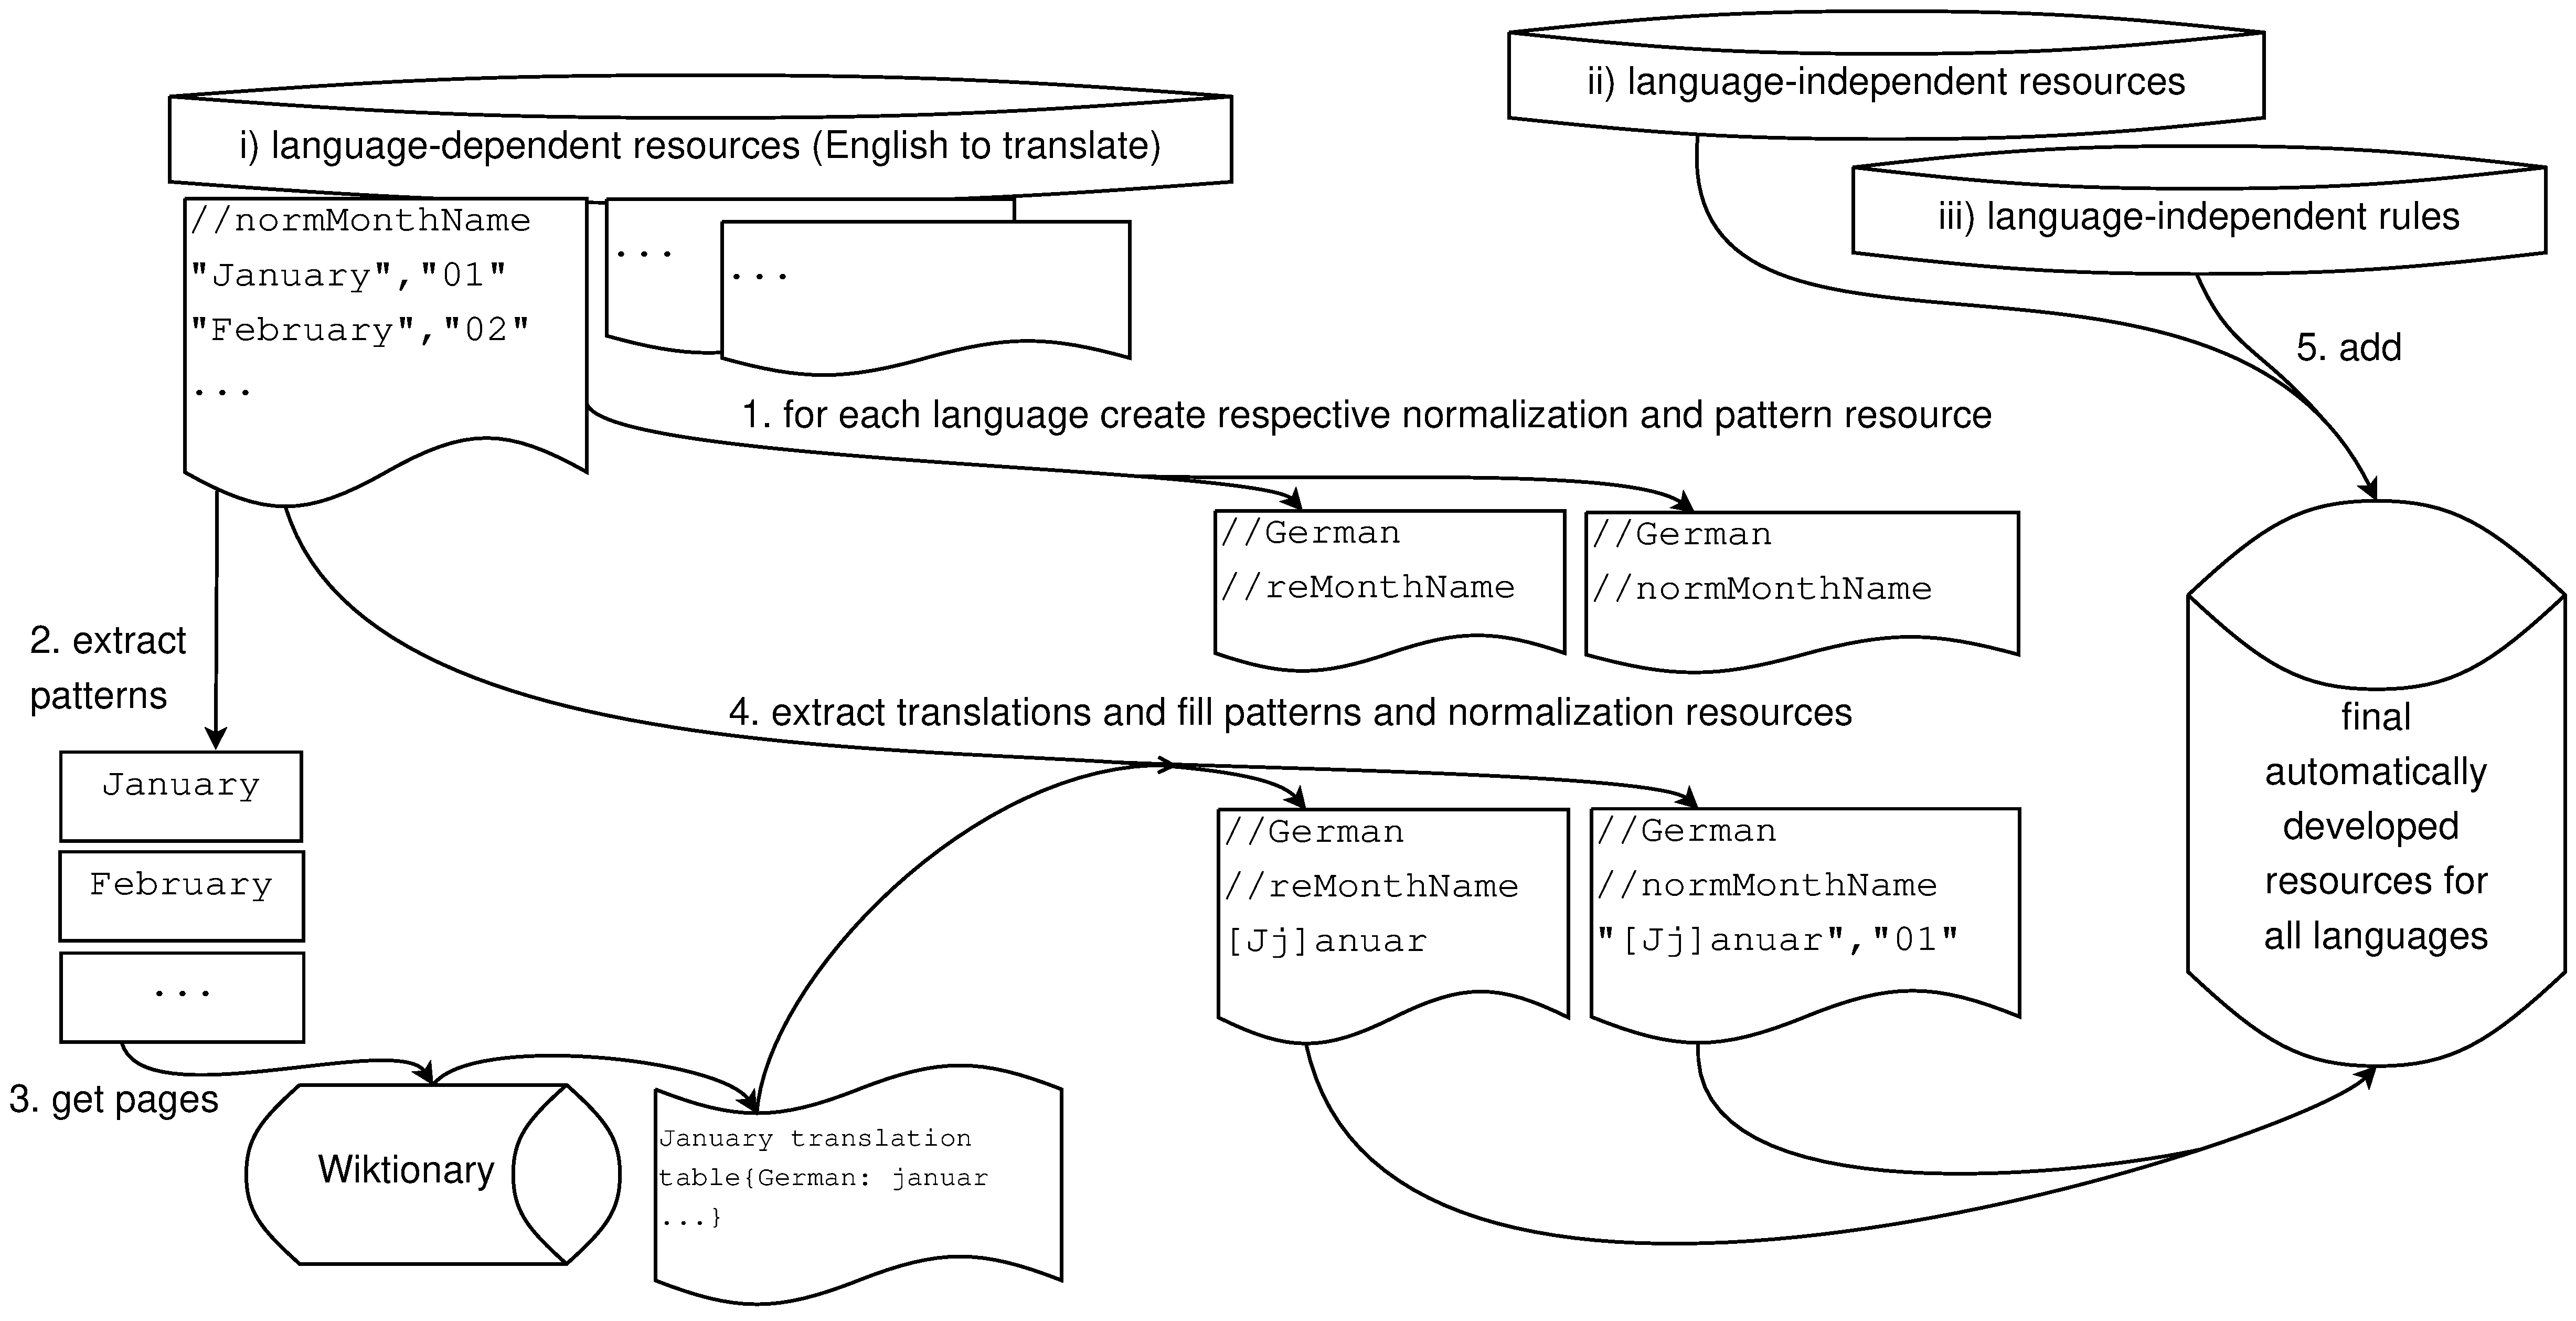
\includegraphics[width=14cm]{Graphics/ht-multilingual}
	\caption{Overview of Mutlilingual HeidelTime Model - adapted from \cite{DBLP:conf/emnlp/StrotgenG15}.}
	\label{figure:3d}
\end{figure}



\section{Multilingual HeidelTime Model Issues} \label{improved-multilingual-ht-model}
The Multilingual HeidelTime Model mentioned in the previous section, allowed HeidelTime to tag documents in many languages that had never been addressed before. These automatically developed resources can be used for baseline temporal tagging or can be a simple starting point to extend them to manual ones for any language. However, it had few shortcomings which we aim to address in this thesis: 

\begin{enumerate}[i.]
	\item Inflection was disregarded for morphologically rich languages in pattern and normalization resources.
	\item Unsegmented languages were not handled by the simplified language independent rules used by all languages.
	\item All languages used the same simplified langauge independent rules, ignoring intricacies of different languages and how temporal expressions might appear in them.
	\item Though not an issue with HeidelTime multilingual model in itself, tagging performance for the languages that lack temporal corpora was not evaluated or analysed.
\end{enumerate}

Now we discuss each of these issues in detail.

\subsection{Disregards Inflections}

The Multilingual HeidelTime model did not take into account the inflections of words for morphologically rich languages such as Polish, Finnish, Turkish, etc. For instance, at present, only translation in the pattern resource reMonthName for Finnish translation of January is [Tt]ammikuu., as shown in the listing below:\\

%\begin{figure}[H]
%	\centering
%	\includegraphics[width=8cm]{fi-reMonthName-ht-221}
%	\caption{reMonthName for Finnish language - using Multilingual HeidelTime Model }
%	\label{figure:3e}
%\end{figure}

\begin{minipage}{\linewidth}
\lstset{caption={reMonthName for Finnish language - using Multilingual HeidelTime Model - version 2.2.1.}, label={listing:3-fi-reMonthName-ht-221}}
\begin{lstlisting}
// english: "January","01"
[Tt]ammikuu
// english: "February","02"
[Hh]elmikuu
// english: "March","03"
[Mm]aaliskuu
// english: "April","04"
[Hh]uhtikuu
// english: "May","05"
[Tt]oukokuu
// ...
\end{lstlisting}
\end{minipage}


While total number of inflections for the Finnish word ``Tammikuu" are around 30, as shown in the Table \ref{table:1f} (page~\pageref{table:1f}). Having all the inflections for this word present in the resource reMonthName for Finnish will allow the rules to extract more temporal expressions. This is the first point we aim to address in this thesis.

\subsection{Ignores Unsegmented Languages}
The Multilingual HeidelTime model used same language independent rules for all languages, as mentioned in Subsection \ref{res-ir} item \ref{res-lir}. As the delimiter used in extraction part of these language independent rules is a space character, it leads to potentially missed extractions in languages that do not have whitespace tokenization between words, such as Thai and Japanese. Addressing rules resources for such languages would also be beneficial. This is the second point we aim to address in the thesis.

\subsection{No Language-specific Rules}
This issue is also related to the same language independent rules for all languages. We aim to learn some frequent temporal patterns as rules for each language and enrich the language independent rules with learned language-specific rules.

There are four types of rules in the language independent rules, i.e., date, duration, set and time, where each type of the rule corresponds to the four values the `type' property of TimeML TIMEX3 tag can take (TimeML is discussed in Subsection \ref{ss2as:timeml}, page \pageref{ss2as:timeml}).

We discuss the four types of language independent rules below:
\begin{enumerate}[i.]
	\item \textbf{Date rules:} The date rules resource file has rules to extract historic dates, complete dates, dates missing year information, names of days and expressions such as `since 1999', etc.
	\item \textbf{Duration rules:} The duration rules resource file has rules to extract temporal expressions such as `two years', `two months', `2 days', etc.  
	\item \textbf{Set rules} The set rules resource file has rules to extract temporal expressions such as `every year', `every month', `every July', etc.
	\item \textbf{Time rules} The time rules resource file has rules to extract temporal expressions such as `morning', `monday morning', `tomorrow morning', `next evening', etc.
\end{enumerate}

As the rules are language independent, some rules are written twice with alternating order of contributing rePattern files in them. For instance, the time rule to extract temporal expressions such as `tomorrow morning' has two rules. The extraction parts of these two rules are \framebox{\%rePartOfDay \%reDateWord} and \framebox{\%reDateWord \%rePartOfDay}. This is done as in some languages rePartOfDay might appear before reDateWord in such time temporal expressions. The two complete rules are given in the Listing \ref{listing:3-lirules} below, with rule name `time\_r1d' and `time\_r1e'.

Moreover, in date rules resource of the language independent rules, only year extraction rule is not present because there is a chance it can detect false positives, i.e., the four digits that do not represent actual year.

In the following listing, we list some of the language independent rules from each of the four types (date, duration, set and time). The comments above the rules give sample temporal expressions in English that can be extracted by respective rules. \\

\begin{minipage}{\linewidth}
\lstset{caption={Some sample language independent rules.}, label={listing:3-lirules}}
\begin{lstlisting}
// r3a: March 30, 2000
// r3b: March 30
RULENAME="date_r3a",EXTRACTION="%reMonthName %reDayNumber,? %reYear4Digit",NORM_VALUE="group(3)-%normMonthName(group(1))-%normDayNumber(group(2))"
RULENAME="date_r3b",EXTRACTION="%reMonthName %reDayNumber",NORM_VALUE="UNDEF-year-%normMonthName(group(1))-%normDayNumber(group(2))"

// r8a: since|until|in 2000
RULENAME="date_r8a",EXTRACTION="%reSinceEtAl %reYear4Digit",NORM_VALUE="group(2)",OFFSET="group(2)-group(2)"

// r2a: two years
RULENAME="duration_r2a",EXTRACTION="%reDayNumberWord4Duration %reUnit",NORM_VALUE="P%normDayNumberWord4Duration(group(1))%normUnit4Duration(group(2))"

// set_r1b: every Monday, each Sunday
RULENAME="set_r1b",EXTRACTION="%reEachEvery %reWeekday",NORM_VALUE="XXXX-WXX-%normDayInWeek(group(2))",NORM_QUANT="%UPPERCASE%(group(1))",NORM_FREQ="1W"

// r1a: morning
RULENAME="time_r1a",EXTRACTION="%rePartOfDay",NORM_VALUE="UNDEF-this-dayT%normPartOfDay(group(1))"

// time_r1d: morning tomorrow
// time_r1e: tomorrow morning 
RULENAME="time_r1d",EXTRACTION="%rePartOfDay %reDateWord",NORM_VALUE="%normDateWord(group(2))T%normPartOfDay(group(1))"
RULENAME="time_r1e",EXTRACTION="%reDateWord %rePartOfDay",NORM_VALUE="%normDateWord(group(1))T%normPartOfDay(group(2))"
\end{lstlisting}
\end{minipage}

Adding some language specific rules to the language independent rules for respective languages can further improve temporal tagging quality of HeidelTime. For instance, a rule that can extract only year temporal expressions, or the most frequently occurring order of complete date for different languages can be beneficial. We aim to learn some language specific rules for different languages, and enrich the language independent rules with those learned rules. This is the third point we aim to address in the thesis.

\subsection{Analysing Language Lacking Temporal Corpora} \label{the-chapter-3-alltc}
Though not an issue with HeidelTime resources, we aim to evaluate the languages that lack temporal corpora using Wikipedia dumps. These analysis results will be an important way to compare performance of the resources we create versus the initial ones, as there are no corpus available for most of the languages.

As Wikipedia dumps are not temporally annotated so there is no way to compute evaluation measures such as precision, recall or f1 score of extraction and normalization, unless we manually tag a subset of the dumps, which is impossible to do for all languages as it requires language experts and creating temporal corpora for even one language is very time and labour intensive. Doing analysis using Wikipedia dumps with different versions of HeidelTime resources can be a meaningful way of comparison between initial and the new resources. This is the fourth point we aim to address in the thesis.

 % HeidelTime theoretical model

\chapter{Implementation of Improved HeidelTime Multilingual Model} \label{the-chapter-4}
In this chapter, we present the implementation of our improved multilingual model for HeidelTime. The starting point of our work, is the model presented by  Str\"{o}tgen and Gertz in \cite{DBLP:conf/emnlp/StrotgenG15}, and also discussed in Section \ref{multilingual-ht-model} of this thesis. We extend the model to address its issues we discussed in Section \ref{improved-multilingual-ht-model}. In this chapter, we discuss the implementation details of our improved model. 

In Section \ref{sec4a}, we discuss the external data sources we use. In Section \ref{sec4b}, we describe how inflections are incorporated. In Section \ref{sec4c}, we discuss how rules for unsegmented languages are adjusted. In Section \ref{sec4d}, we explain the learning of language specific rules. 

%	\textcolor{violet}{some intro ...}

\section{Data Sources} \label{sec4a}
We use external sources such as online dictionaries and word embeddings to get inflections for morphologically-rich languages. Moreover, to learn language specific frequently occurring patterns as rules, we use Wikipedia. 


\subsection{Wiktionary}
Wiktionary, made available by the Wikimedia Foundation, is a \textit{web-based project to create a free content dictionary of all words in all languages}\footnote{\url{https://en.wikipedia.org/wiki/Wiktionary}}. Like other sites of Wikipedia, it is collaboratively edited via wiki by volunteers, that are not necessarily language experts. The content of a usual Wiktionary article may give information about a word's part-of-speech, etymology, definitions, example usage sentences, pronunciations, translations, synonyms/antonyms, among others \cite{navarro2009wiktionary}. For certain words of morphologically-rich languages, inflections may also be provided.
	
The translation section for a word on Wiktionary article can contain multiple translation tables, if the word has more than one meanings in English. For instance, the month name ``May" has more than one meaning in English, i.e., the fifth month of the Gregorian calendar, the name of a hawthorn flower or a given name; so the English wiktionary page for May has three translation tables\footnote{\url{https://en.wiktionary.org/wiki/May\#Translations}}, one for each of the mentioned meaning. These are the translation tables, that are used by the present HeidelTime multilingual model \cite{DBLP:conf/emnlp/StrotgenG15} to extract translations in various languages (the third step in Figure \ref{figure:3d}).
	
As mentioned earlier, Wiktionary may also provide inflection tables, for words that have inflections. Continuing from the example of the English wiktionary page for the word ``May", in the translation table for the sense, i.e., fifth month, translations in various languages are given. For instance, next to Turkish, the translation is given as ``mayıs", that points to its own page\footnote{\url{https://en.wiktionary.org/wiki/may\%C4\%B1s\#Turkish}}, that describes the word ``mayıs", and also provides an inflection table for it. As the present HeidelTime multilingual model already gets the translation ``mayıs" from the page for May, the next step should be to extend it further so as to also get the inflections for the word ``mayıs'' from its page. 

On analysing Wiktionary, we found that it provided inflections tables for the words in languages such as Finnish, Turkish, Polish, etc.  The words in these languages we looked for were the translations in respective languages for the words as given in the simplified English normalization resources (Subsection \ref{res-ir} \ref{res-ir-i}). For instance, the month names in Finnish, Turkish and Polish all had inflection tables available on Wiktionary. 
	
\subsection{FastText}
FastText\footnote{\url{https://fasttext.cc/}}, by Facebook Research, is a highly multilingual library for efficient learning of word representations and text classification. FastText is a library that provides word embeddings, also known as word vectors or distributed representation, for words. Word embedding libraries embed words in a vector space model, thereby representing each word by a vector, such that semantically similar words have vectors that are closer to each other. 

FastText learns representations for character n-grams, and represent words as as the sum of the learnt character n-gram vectors \cite{DBLP:journals/tacl/BojanowskiGJM17}. FastText takes into account the morphology of words by having many vectors for different parts of a word (n-grams). In addition to utilizing character level information to improve word vectors, FastText also has made available pre-trained word vectors for 294 languages\footnote{\url{https://fasttext.cc/docs/en/pretrained-vectors.html}}. 

FastText has been shown to perform on par with recent deep learning methods in the tasks of text classification and sentiment analysis, while being much faster \cite{DBLP:journals/corr/JoulinGBM16}. Similarly, it was also shown to perform very well for the tasks of word similarity and word analogies \cite{DBLP:journals/tacl/BojanowskiGJM17}. 

FastText also provides an interface to find the nearest neighbors of a word. Given a word as input, it returns a list of similar words ranked by their cosine similarity scores. This can be used to get interchangeable words for a word, or to simply validate the quality of learnt word vectors by looking at the nearest neighbors for some words. We looked at the nearest neighbor functionality for languages such as Finnish, Estonian and Turkish, and found out that it consistently returning the inflections of words in the list of top ten nearest neighbor words, though related words that are not inflections were also returned.

\subsection{Wikipedia}
Wikipedia, made availabe by the Wikimedia Foundation, is a \textit{free online encyclopedia with the mission of allowing anyone to edit articles}\footnote{\url{https://en.wikipedia.org/wiki/Wikipedia}}. It is available in 299 languages, and is ranked fifth most popular website\footnote{\url{http://www.alexa.com/siteinfo/wikipedia.org}}. Of the 299 languages Wikipedia is available in, 13 of these have over one million articles each\footnote{\url{https://en.wikipedia.org/wiki/Wikipedia\#Language\_editions}}. Full details about the number of articles available in each language can be seen at the link\footnote{\url{https://meta.wikimedia.org/wiki/List\_of\_Wikipedias}}.

Wikipedia has made available the dumps\footnote{\url{https://dumps.wikimedia.org/}} in various formats such as XML, SQL, etc. These can be downloaded for all the languages Wikipedia is available in. We aim to make use of these dumps for the tasks of learning frequently occurring temporal expressions for different languages and for the analysis of languages that lack temporally annotated coropora. 
\section{Getting Inflections} \label{sec4b}
As mentioned earlier, in Section \ref{morphologically-rich-languages-background} (page \pageref{morphologically-rich-languages-background}), morphologically-rich languages are such that have rich morphology of words in them or inflection of words. As of HeidelTime version 2.2.1, the pattern resources of current HeidelTime do not have the inflections of words in them for such languages. This renders the useful rules, in language independent rules for such languages, useless as they are not able to extract patterns due to missing inflections in respective pattern resources.  

For instance, a simple date rule, in automatically developed resources for extracting dates like ``16 August 2003" with punctuations and few tokens allowed in between is given in the following listing. \\

% zebra color effect following commented lines, but the mess up referencing labels of these lstings	
%\begin{lstlisting}[
%caption={A language independent rule to extract dates - showing only extraction part of the rule},
%label={listing:4a}
%identifierstyle=\oddtest,
%commentstyle=\oddtest,
%stringstyle=\oddtest,
%keywordstyle=\oddtest,
%linebackgroundcolor={\ifodd\value{lstnumber}\color{cream}\fi}
%]
%// r1a: 30 August 2000 (with "." and "," etc allowed between)
%%reDayNumber\.?( [\S][\S]?)? %reMonthName,?( [\S][\S]?)? %reYear4Digit
%\end{lstlisting}

\begin{minipage}{\linewidth}
\begin{lstlisting}[
caption={A language independent rule to extract dates - showing only extraction part of the rule.},label={listing:4a}]
// r1a: 30 August 2000 (with "." and "," etc allowed between)
%reDayNumber\.?( [\S][\S]?)? %reMonthName,?( [\S][\S]?)? %reYear4Digit
\end{lstlisting}
\end{minipage}


Now let us consider the following Finnish text\footnote{The Finnish text excerpt is taken from Wikipedia, see \url{https://fi.wikipedia.org/wiki/?curid=30}}:

%\begin{figure}[H]
%	\centering
	\begin{mdframed}[style=MyFrame]
		\raggedright{
			Antti Johannes Satuli (\ul{8. lokakuuta 1946} Helsinki – \ul{17. huhtikuuta 2003} Inari) oli oikeustieteen kandidaatti, joka loi uransa Suomen ulkoasiainministeriön palveluksessa. Hän oli Suomen ensimmäinen suurlähettiläs ja pysyvä edustaja Euroopan unionissa siihen liittymisen jälkeen. Vuonna 2002 hänet nimitettiin ulkoministeriön valtiosihteeriksi.
		}
	\end{mdframed}
%	\caption{a sample Finnish text excerpt}
%	\label{figure:4-finnish-text-excerpt}
%\end{figure}

We can see that above Finnish excerpt has two dates in it that are underlined. The rule given in Listing \ref{listing:4a} is perfectly capable of extracting the dates underlined in above given Finnish text. However, these dates are not extracted by the HeidelTime as of version 2.2.1, as the month names in those dates, i.e., ``lokakuuta" and ``huhtikuuta" are inflections of the nominative forms, i.e., ``lokakuu" and ``huhtikuu" respectively. Since, only the nominative forms of months are present in Finnish reMonthName pattern file for Finnish, as of HeidelTime 2.2.1, these dates are not extracted (see\footnote{The inflection and cases information about month names in Finnish language being discussed here is taken from wiktionary: \url{https://en.wiktionary.org/wiki/huhtikuu\#Finnish} and \url{https://en.wiktionary.org/wiki/lokakuu\#Finnish}; we are not native speakers of the language}). 

If reMonthName for Finnish is created such that it has the inflections in it the same rule given in Listing \ref{listing:4a} will successfully extract the underlined temporal expressions in sample Finnish text given above. We aim to create pattern files such that they contain such inflections for morphologically rich languages. 

We make use of the external sources of Wiktionary and FastText to get inflections, and put them in pattern resources of automatically developed resources for HeidelTime. 

\subsection{Getting Inflections Using Wiktionary} \label{sec4b1}
The first approach we take to get inflections is to use Wiktionary as a data source. This approach can be considered as a direct extension of the current Multilingual HeidelTime model, discussed in Section \ref{multilingual-ht-model} (page~\pageref{multilingual-ht-model}), to create automatically developed resources. We extend the multilingual model to get inflections for the words we are translating, if they exist. 

For the sake of completeness, below we restate all the steps with our extension step (\ref{extension-step-3a}):

\begin{enumerate}[1.]
	\item We create pattern and normalization resources, for each language, using the language dependent resources. These pattern and normalization resources are empty at the end of this step.
	\item We then get all the patterns (English words to translate) from the language dependent resources. 
	\item We then crawl each respective Wiktionary page of the patterns (English words to translate) and get the translation for the patterns from the translation tables present on Wiktionary. For instance, for month name January, we get the translation tammikuu for Finnish language in this step. Similarly, we get translations for all the pattern words in all languages.  
		\begin{enumerate}[a.]
		\item \label{extension-step-3a} This step is the extension we add to current multilingual model of HeidelTime. Here we crawl the page of respective translations of the patterns, and get all inflections from the inflection table if they exist. For instance, for Finnish language, we go to the Wiktionary page for ``tammikuu'', and get all its inflections such as tammikuut, tammikuun, etc. from its inflection table. Similarly, we get inflections for other words and for other languages. 
		\end{enumerate}
	\item We then fill the empty pattern and normalization files, created in first step, with the found translation words and their inflections. 
	\item Finally, we add the language independent resources and language independent rules to the created resources for each language in previous step to get the final automatically developed resources for all languages. 
\end{enumerate} 

The following figure gives an overview of all these steps to create automatically developed resources. It is identical to the Figure \ref{figure:3d} (page~\pageref{figure:3d}), except for the additional step that is shown as highlighted. 

\begin{figure}[H] 
	\centering
	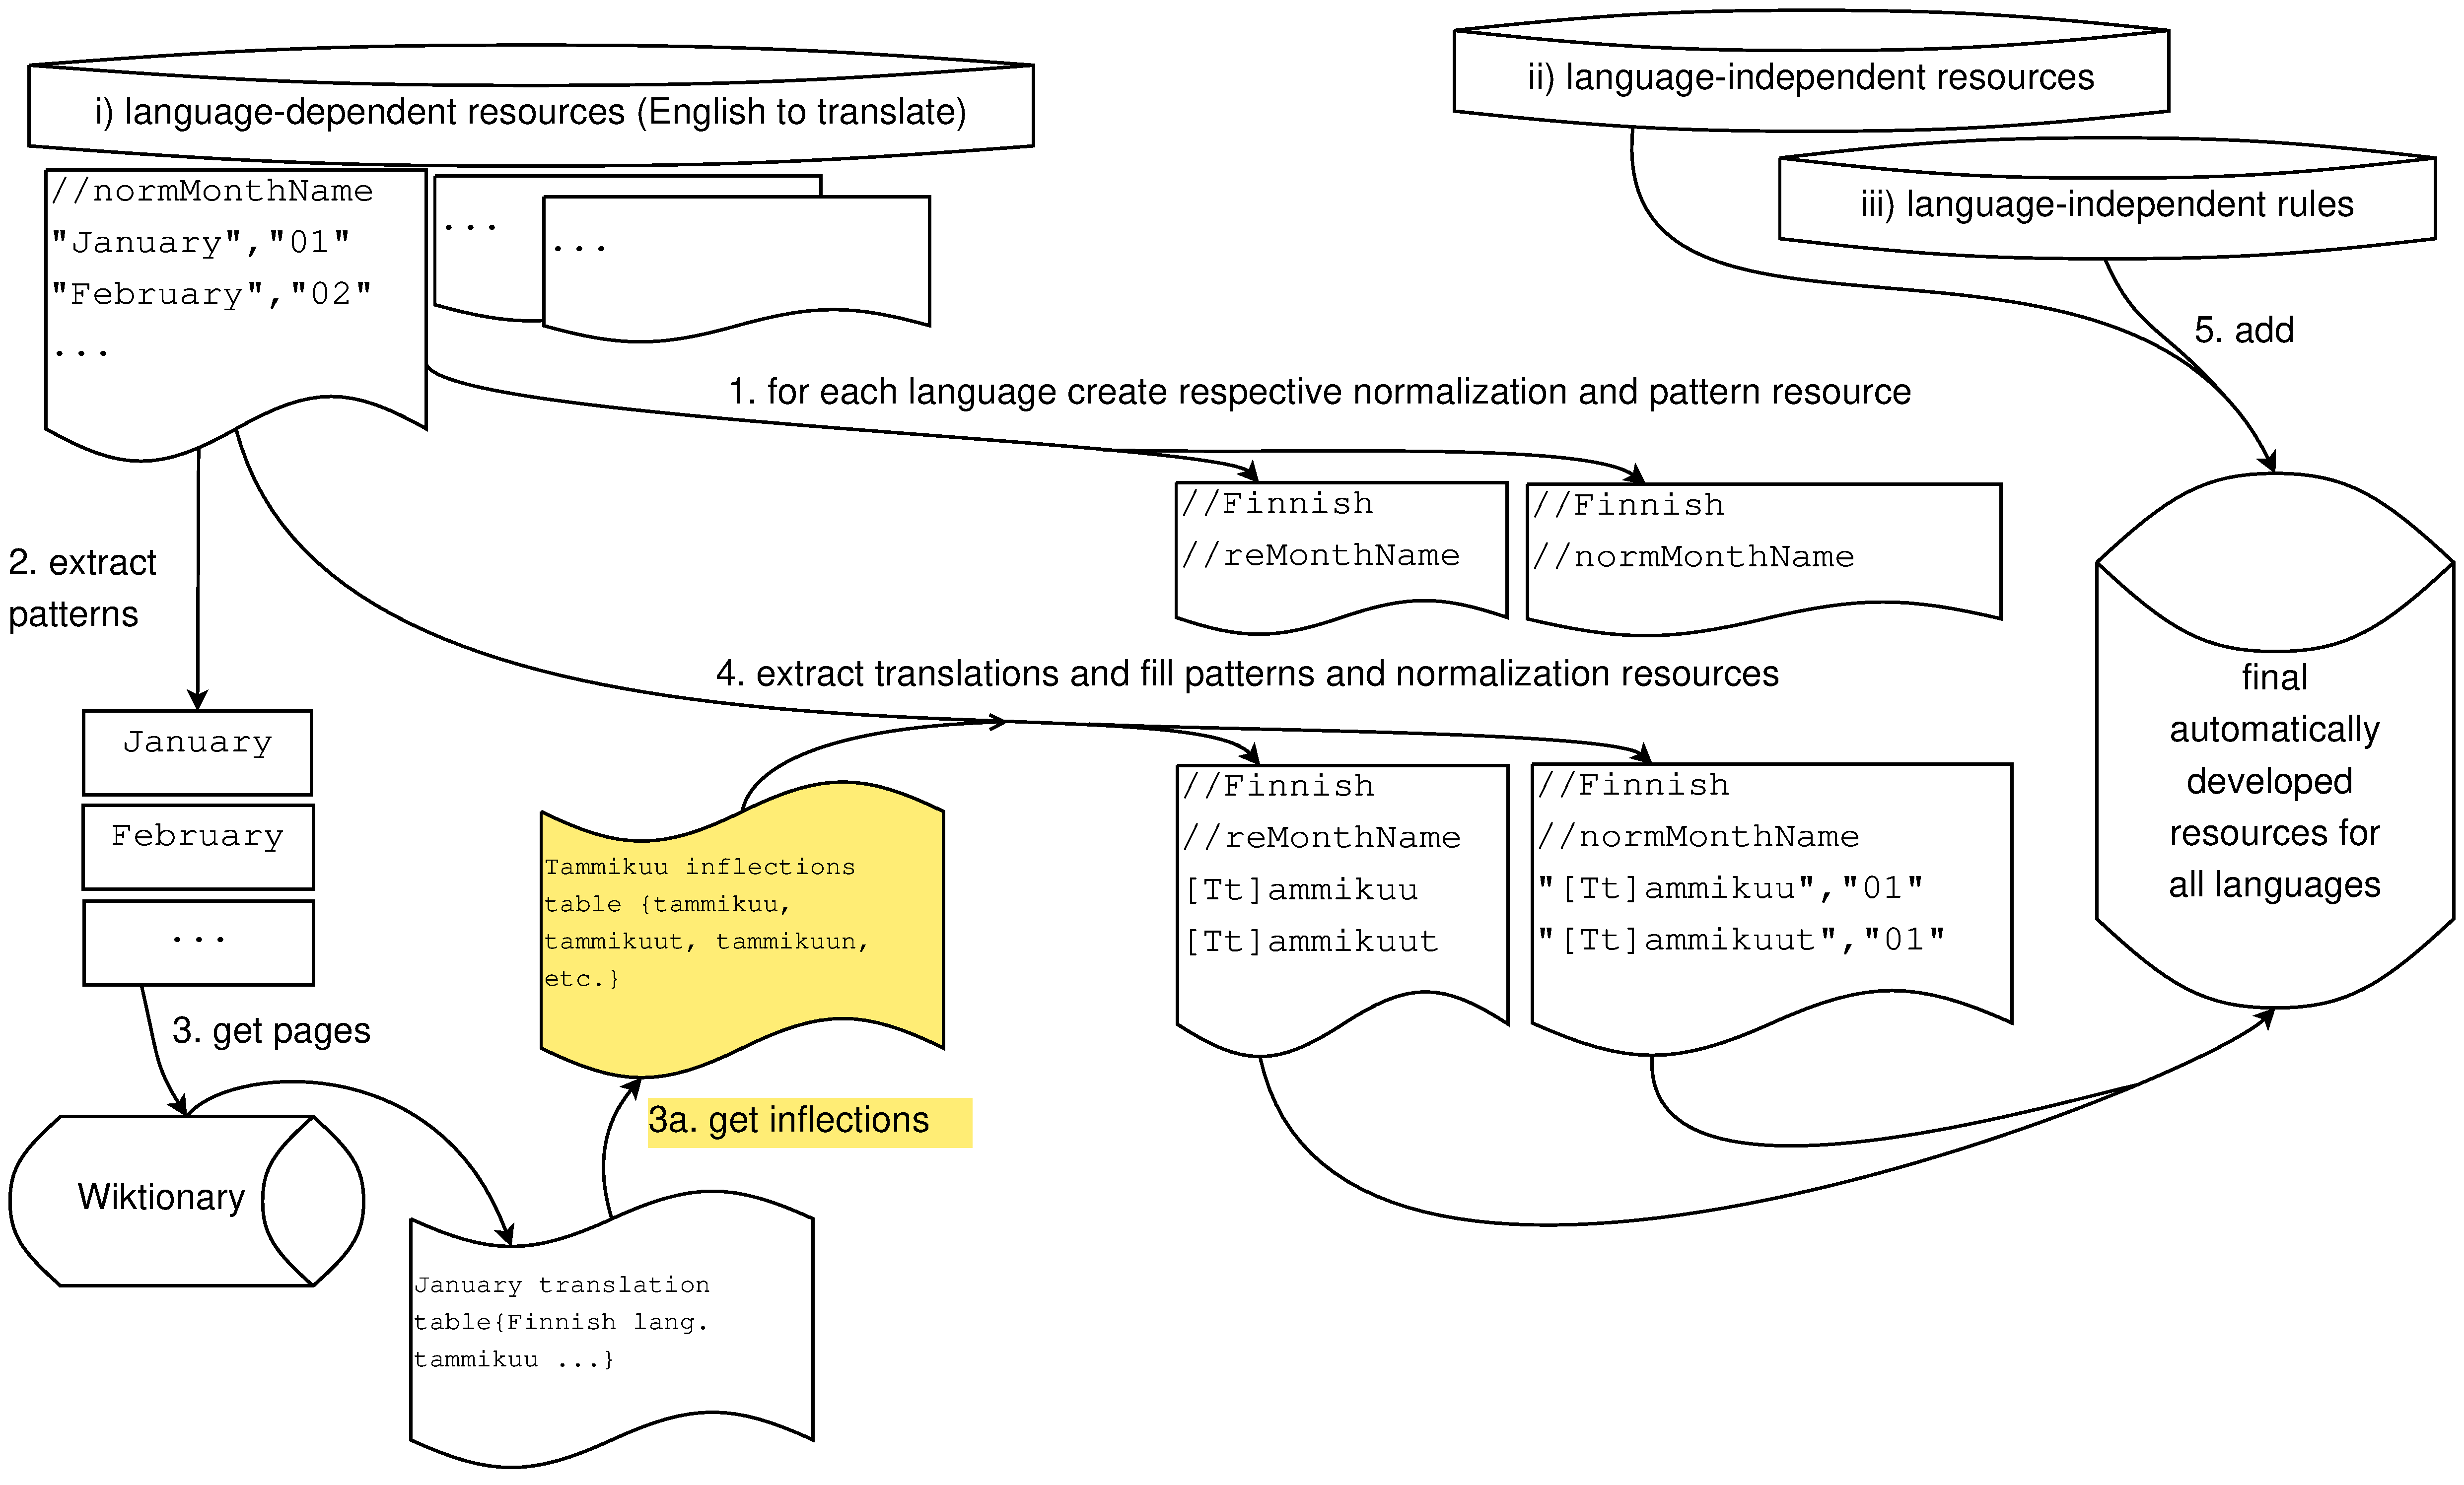
\includegraphics[width=14cm]{Graphics/ht-multilingual-new-1}
	\caption{Overview of Improved Mutlilingual HeidelTime Model - Getting Inflections - using Wiktionary.}
	\label{figure:4a}
\end{figure}

\textbf{Resulting Resources}\\
Once we run the improved multilingual model discussed above, we get the automatically developed resources for all languages contain inflections in their pattern and normalization files. We observed the resulting pattern files for morphologically rich languages and found that the inflections were successfully extracted from Wiktionary. For instance, the Listing \ref{listing:4-fi-2x-wiktionary} below shows part of pattern file reMonthName for Finnish language using our new improved multilingual model:\\


%\begin{figure}[H]
%	\centering
%	\includegraphics[width=8cm]{fi-reMonthName-ht-2x-wiktionary}
%	\caption{reMonthName for Finnish language - using Improved Multilingual HeidelTime Model - using Wiktionary}
%	\label{figure:4b}
%\end{figure}

\begin{minipage}{\linewidth}
\begin{lstlisting}[caption={reMonthName for Finnish language - using Improved Multilingual HeidelTime Model - using Wiktionary.},label={listing:4-fi-2x-wiktionary}]
// english: January, 01
[Tt]ammikuu
[Tt]ammikuusta
[Tt]ammikuiden
[Tt]ammikuuksi
[Tt]ammikuissa
[Tt]ammikuitten
[Tt]ammikuuhun
// ...
\end{lstlisting}
\end{minipage}

We can see that our improved model extracted all the inflections for month name ``Tammikuu", as compared to the only base word ``Tammikuu" being extracted by the multilingual model, as of HeidelTime version 2.2.1 (c.f. Listing \ref{listing:3-fi-reMonthName-ht-221}, page \pageref{listing:3-fi-reMonthName-ht-221}). 
\subsection{Getting Inflections Using FastText} \label{sec4b2}
The second approach we take to get inflections is to use FastText's nearest neighbor functionality. The overall model is again similar to the original model, except now instead of Wiktionary we make use of Yandex.Translate\footnote{\url{https://translate.yandex.com/}} service and FastText library. We use Yandex online translator instead of other translators such as Google or Microsoft because it is available freely; moreover, we also get to create resources developed using a resource other than Wiktionary. In addition, we use FastText because it is an open-source and lightweight library that provides multilingual word vectors for over 150 languages; and provides functionality that returns nearest neighbors of an input word, which we aim to use to get inflections of words in morphologically rich languages.

Following, we only state the steps that are performed differently than when getting inflections using Wiktionary model.

\begin{enumerate}[1.]
	\setcounter{enumi}{2}
	\item For each of the patterns (English words to translate), get their translation from Yandex Translate. For instance, for month name January, we get the translation Tammikuu for Finnish in this step. Similarly, we get translations for all the pattern words for all languages. 
	\begin{enumerate}[a.]
		\item Here we take the translation we got from previous step and get nearest neighbors of the translation using FastText. For instance, for the translated word Tammikuu in Finnish, we get some relevant inflections for it such as Tammikuulla, and we also get some relevant words but not inflections such as Helmikuu (February in Finnish language).  
		\item As some relevant words might be returned by FastText that are not inflections, so we translate the returned words again using Yandex Translate, and verify if they indeed translate back to the original pattern. For instance, the returned relevant inflection word Tammikuulla by FastText will translate back to January; however, the returned relevant word but not inflection, i.e., Helmikuu, will not translate back to January. 
	\end{enumerate}
\end{enumerate}

The rest of steps are similar to the model to get inflections using Wiktionary (Figure \ref{figure:4a}). The following figure gives an overview of all these steps to create automatically developed resources using FastText. It is identical to the Figure \ref{figure:4a} (page~\pageref{figure:4a}), except for the highlighted steps. 

\begin{figure}[H] 
	\centering
	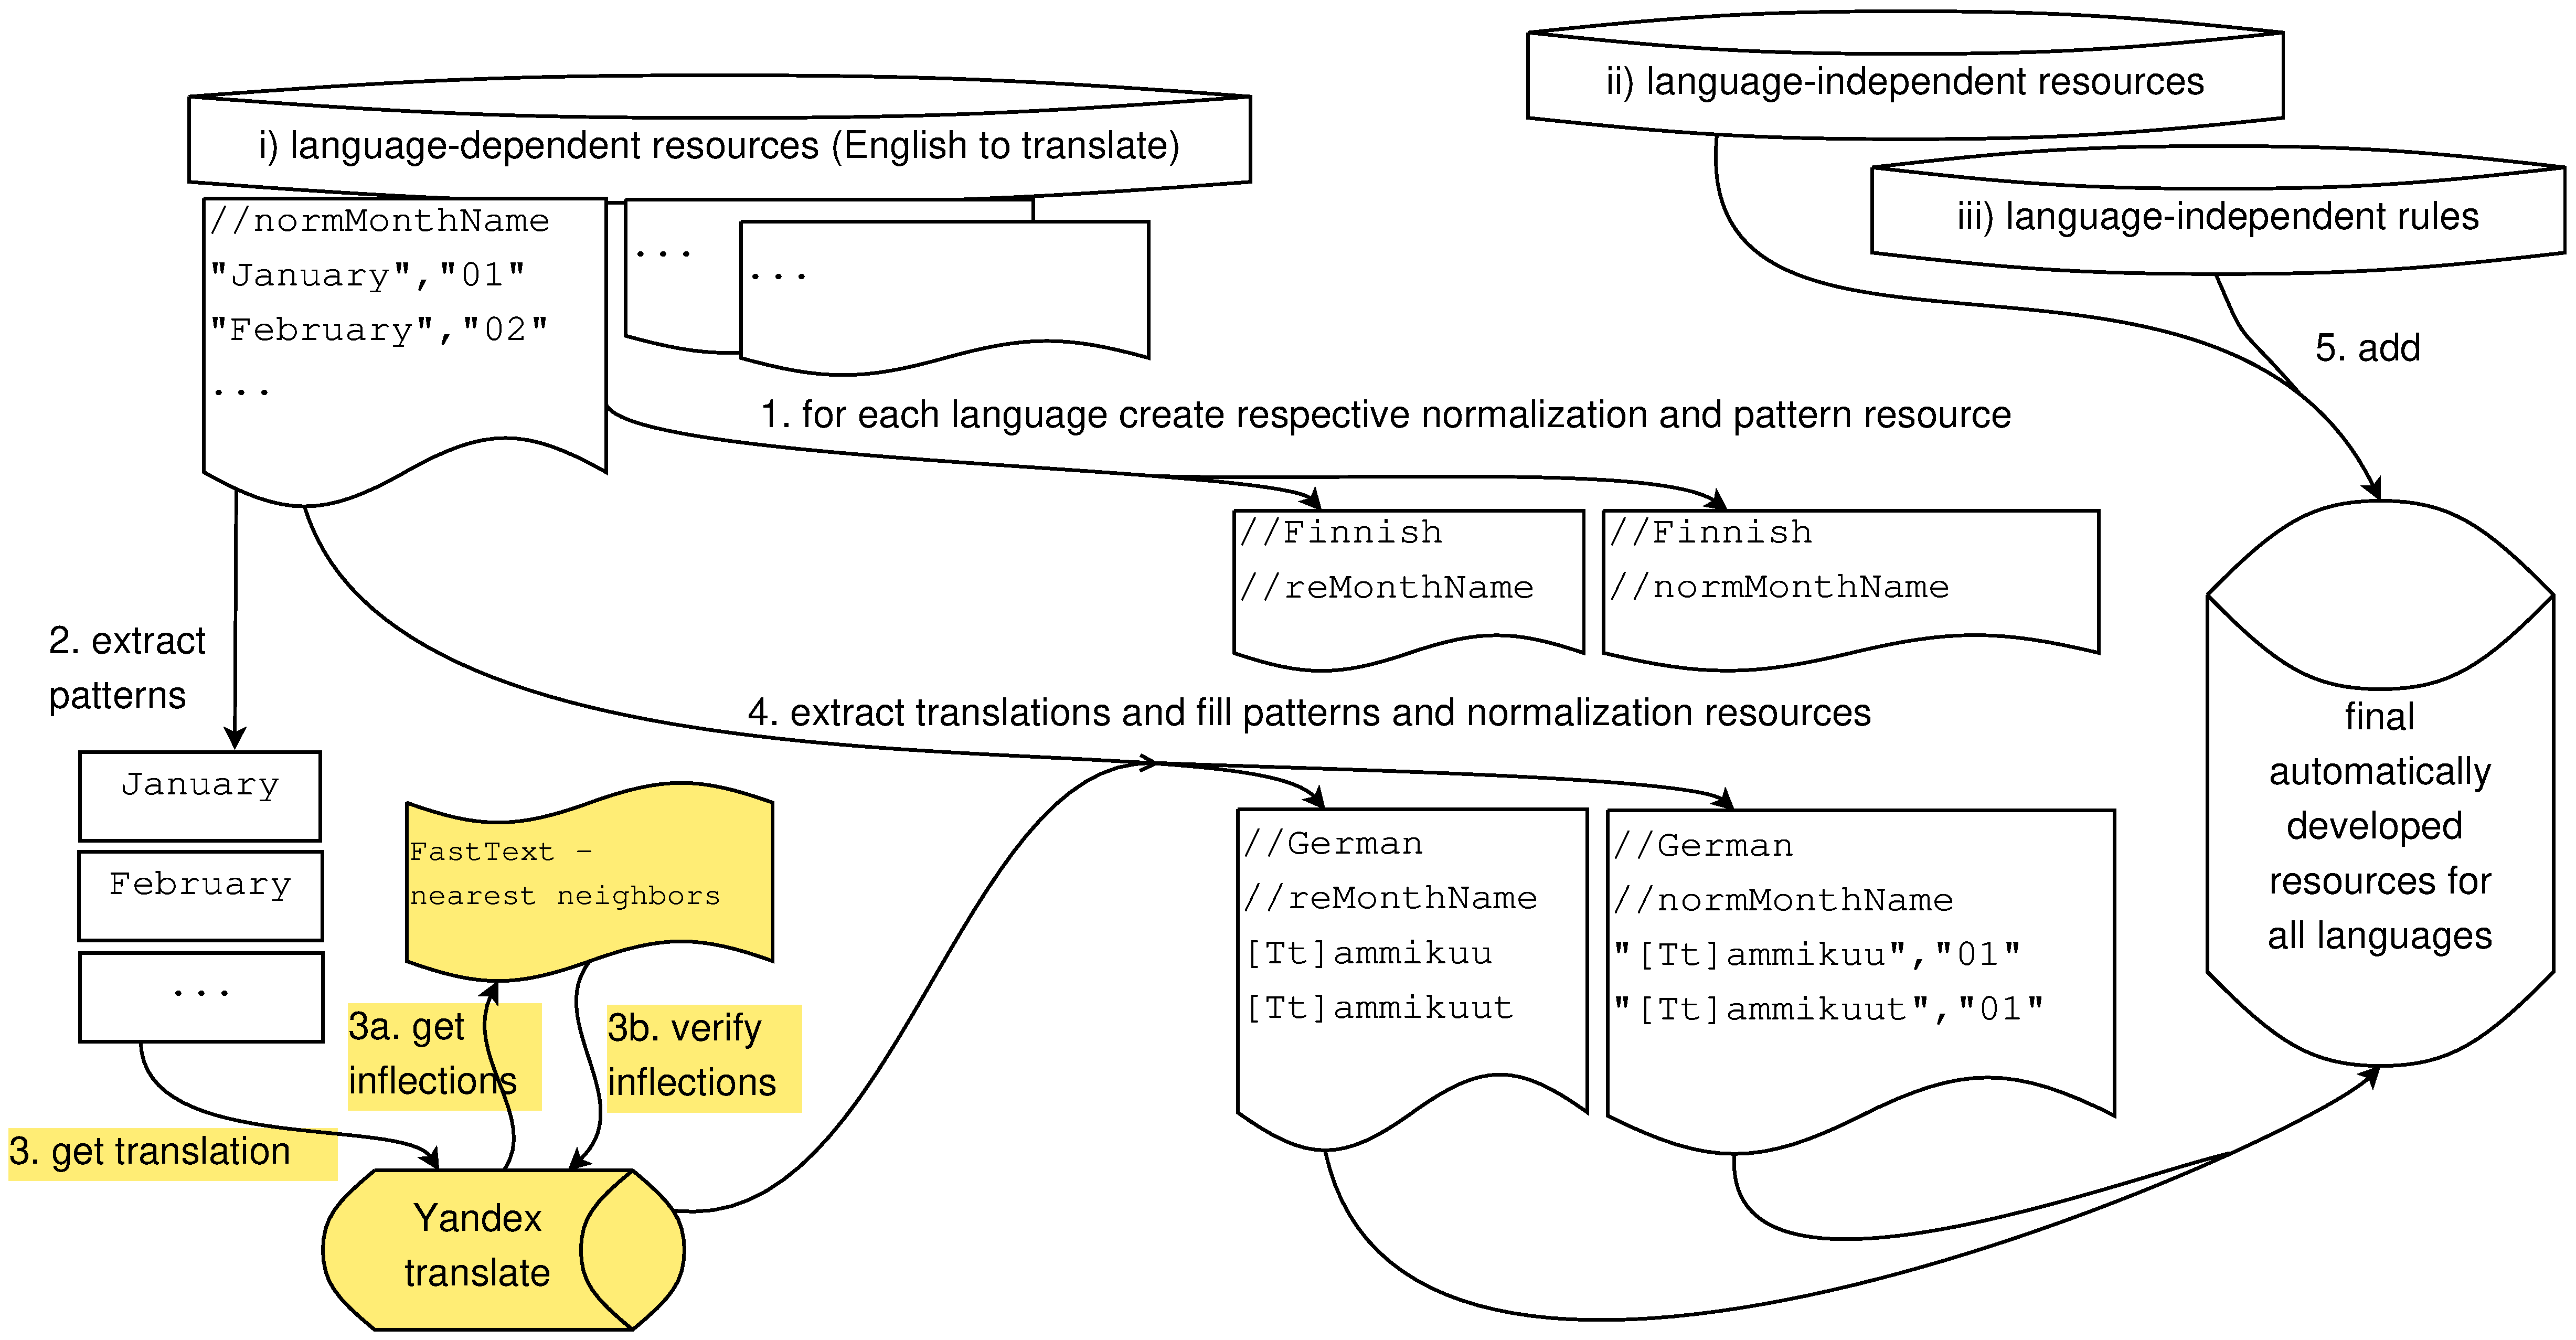
\includegraphics[width=14cm]{Graphics/ht-multilingual-new-2}
	\caption{Overview of Improved Mutlilingual HeidelTime Model - Getting Inflections - using FastText.}
	\label{figure:4c}
\end{figure}

\textbf{Resulting Resources}\\
Once we run the improved multilingual model discussed above, using word vectors of a certain language, we get the automatically developed resoruces for that language. The created pattern and normalization resources have inflections in them for morphologically rich languages. We compared the resulting resources for some of the morphologically rich languages and found that, though inflections were being extracted and written in resources, they were less in number than those obtained by the earlier model that used Wiktionary as a data source to get inflections. For instance, the following Listing \ref{listing:4-fi-2x-ft} shows part of pattern file reMonthName for Finnish language that is created using our improved multilingual model that uses FastText as data source:\\

\begin{minipage}{\linewidth}
\begin{lstlisting}[caption={reMonthName for Finnish language - using Improved Multilingual HeidelTime Model - using FastText.},label={listing:4-fi-2x-ft}]
// english: "January","01"
[Tt]ammikuu
[Tt]ammikuuta
[Tt]ammikuut
// english: "February","02"
[Hh]elmikuuta
[Hh]elmikuu
[Hh]elmiku
// ...
\end{lstlisting}
\end{minipage}

We can see that even though inflections are extracted, but they are less than the number of inflections in Finnish rePatternFile file created using earlier model that used Wiktionary (c.f. Listing \ref{listing:4-fi-2x-wiktionary}). It might be the case that FastText method gives us better rePattern files for some languages as compared to the Wiktionary method; this will be discussed in the evaluations we run in the Chapter \ref{the-chapter-5}.

\section{Accommodating Unsegmented Languages} \label{sec4c}
As of HeidelTime version 2.2.1, the automatically developed resources of all languages use the same language independent rules. These rules are simplified rules and use space as a separator between different temporal expressions in a rule. 

For instance, extraction part of a simple date rule in the simplified rules is:\\


%\begin{lstlisting}[
%caption={A simple language independent rule to extract dates - showing only extraction part of the rule},label={listing:4b}
%identifierstyle=\oddtest,
%commentstyle=\oddtest,
%stringstyle=\oddtest,
%keywordstyle=\oddtest,
%linebackgroundcolor={\ifodd\value{lstnumber}\color{cream}\fi}
%]
%%reMonthName %reDayNumber,? %reYear4Digit
%\end{lstlisting}

\begin{minipage}{\linewidth}
\lstset{caption={A simple language independent rule to extract dates - showing only extraction part of the rule.},label={listing:4b}}
\begin{lstlisting}
// rule to extract dates like January 20, 2002
%reMonthName %reDayNumber,? %reYear4Digit
\end{lstlisting}
\end{minipage}

%\begin{mdframed}[style=MyFrame]
%	\begin{verbatim}
%	%reMonthName %reDayNumber,? %reYear4Digit
%	\end{verbatim}
%\end{mdframed}

The rule in Listing \ref{listing:4b} extracts temporal expressions that appear in following order, i.e., reMonthName followed by space followed by reDayNumber followed by an optional comma followed by space and finally reYear4Digit. Thus, we can see this rule assumes space as separator between the parts of a date. This extraction pattern ignores the unsegmented languages and would not extract temporal expressions in such languages. We refer to similar date rule for Chinese language, as given in manually created Chinese resources of HeidelTime \cite{DBLP:conf/eacl/LiSZG14}. The similar rule in Chinese given in manual HeidelTime resource is:\\

\begin{minipage}{\linewidth}
\lstset{caption={A manually developed Chinese rule to extract dates - showing only extraction part of the rule.},label={listing:4c}}
\begin{lstlisting}
// EXAMPLE date_year_c5: 一九八七十二月二十八日
(%reYear4Digit|%reYear2Digit)年(%reMonthWord)(%reDayWord日)
\end{lstlisting}
\end{minipage}

%\begin{mdframed}[style=MyFrame]
%	\begin{verbatim}
%	%reYear4Digit年%reMonthWord%reDayWord日
%	\end{verbatim}
%\end{mdframed}

%\begin{figure}[H]
%	\centering
%	\begin{mdframed}[style=MyFrame]
%		\begin{verbatim}
%		%reYear4Digit年%reMonthWord%reDayWord日
%		\end{verbatim}
%	\end{mdframed}
%	\caption{a Chinese date rule}
%	\label{figure:4-chinese-date-rule}
%\end{figure}


In Listing \ref{listing:4c}, we see that the actual manual Chinese rule has separator words between the rePatterns (\%reYear4Digit, \%reMonthWord and \%reDayWord). The separator words used are 年 and 日, where 年 translates to `year' and 日 translates to `day'. 

Our first approach to cater the unsegmented languages is to simply remove the spaces in the simplified language independent rules for such languages, but as we can see from the above example, the space might be replaced by actual words like 年 and 日, at least in one of the complete date rule. In the next section, we present our approach to learn frequently occurring temporal patterns as rules for all languages, that might enable us to learn better rules for unsegmented languages too (For instance, a rule similar to the one in Listing \ref{listing:4c} for Chinese language). 

\section{Learning Language-specific Rules} \label{sec4d}
In this section, we discuss how the new rules are learned for different languages from frequently occurring temporal expressions in them. The learnt language specific rules are then appended to the language independent rules. The aim is to enrich the simplified language independent rules for automatically developed resources of all languages with language-specific rules of respective languages. Another way to put it is that the aim is to learn some language dependent rules by analysing Wikipedia dumps of respective languages, and append those to the simplified language independent rules. Thus, making the simplified rules language dependent and improving extraction quality. That is, the new rules will be language dependent, but as the previous extension to new languages, automatically created.

One issue with the language independent rules, for automatically developed HeildelTime resources, is that they do not have a rule for dates that have year granularity. Since using just four digit numbers might be too ambiguous and thus result in many false positives, and, without language specific information, no extended rules can be added. For instance, the temporal expressions that represent four-digit years, without month information, such as ``2004" are not extracted for any language. This is an understandable decision, because it is not necessary that every four digits refer to a year. For instance, in ``there were around 2000 spectators", 2000 does not represents the year 2000. However, if the four-digit years occur near the keyword ``year", then the four-digit number certainly refers to respective year, and is a temporal expression that should be extracted. One of our goal, in learning language specific rules, is to learn such only year rules. 

It is likely that only year rule will be a permutation of the patterns ``reYearToken" and ``reYear4Digit" and possibly some other word or punctuation. For instance, in German language the extraction part of only year rule should be:\\
\framebox{\%reYearToken \%reYear4Digit}\\
This can extract German temporal expressions such as ``Jahr 2009", assuming reYearToken pattern has the translation ``Jahr" available in it. 

It is equally likely that the four-digit year appears with some word other than the year token; for instance, in English consider the sentence ``He was born in 1934". Here the four-digit year appears with the English word ``in". As of HeidelTime version 2.2.1, there is no pattern file in English-to-translate initial resources that has word ``in" in it. Moreover, even if such file is present, there is a chance that no correct translation for any language is found while creating pattern resources for that language using Wiktionary or FastText. For instance, the Finnish word ``vuonna" translates to ``in the year"\footnote{using Wiktionary, i.e., \url{https://en.wiktionary.org/wiki/vuonna}} in English language. And the word ``vuonna" is not found by our system on wiktionary while crawling it, i.e., no pattern resource file of Finnish has the word ``vuonna" in it; so for such cases, only year rules can be made that have the word of a language itself in the rule, as compared to \%rePattern names. For instance, in Finnish language only year rule's extraction part can be:\\
\framebox{[Vv]uonna \%reYear4Digit }\\
This can extract Finnish temporal expressions such as ``vuonna 1984".

Another rule that can be learned is the complete date rule for unsegmented languages. As discussed in Section \ref{sec4c}, the simplified language independent rules do not work on unsegmented languages, because these rules assume space a delimiter between date parts or some other punctuations or small words. For instance, we aim to learn rule such as the one shown in Listing \ref{listing:4c} for Chinese language, that uses the Chinese words, i.e., 年 and 日, as separators between date parts. 

Now, we discuss our approach of analysing Wikipedia dumps for different languages to learn language dependent rules based on frequently occurring temporal expressions in respective languages. 

\subsection{Learning Language-specific Rules using Wikipedia}
The approach we take to learn language specific rules for different languages makes use of Wikipedia as a data source. As mentioned earlier, Wikipedia articles have ample temporal information in them and are readily available to download as dump files for different languages. We used the Wikipedia dumps having version 20171020 (dated 2017-10-20), for 177 languages that had this version available to download, to learn language-specific rules for these languages.

Following, we discuss our pipeline to learn rules from frequently occurring temporal expressions. 

\begin{enumerate}[1.]
	\item We get the Wikipedia dump of a language from Wikipedia dumps website\footnote{\url{http://dumps.wikimedia.your.org}}, that are in .xml.bz2 format\footnote{for instance, the Finnish wiki dump we used is available at  \url{http://dumps.wikimedia.your.org/fiwiki/20171020/fiwiki-20171020-pages-articles-multistream.xml.bz2}}, and run a script\footnote{script by Giuseppe Attardi, available at \url{https://github.com/attardi/wikiextractor}} that extracts the texts from the dumps and add them to a MongoDB collection of respective language. 
	
	\item We then set up HeidelTime UIMA pipeline, that we use to tag the Wikipedia articles of respective language's MongoDB collection, using base rules (language independent rules that have individual \%rePatterns as extraction part, see Listing \ref{listing:4d} below). This step tags all the individual temporal patterns found and puts the result in a new collection in MongoDB.
	
	\item  We then analyse the collection created in previous step. It has all the individual temporal expressions tagged separately using base rules. For instance, if two or more temporal expressions appear in close proximity of one another, we note the words or punctuations that appear between these temporal expressions. A dictionary like structure is made that has a tuple as key, that has the two contributing temporal expressions, and has dictionary as value that stores the words and their counts they appear between the two temporal expressions (see Listing \ref{listing:4e}). Similar dictionary structures to maintain the words that appear before and after an extracted  individual temporal pattern are also made. 
	
	Only the most frequently occurring word or punctuation between two indivdual temporal expressions is used as token between the contributing temporal patterns for the new rule; this makes sure that the learned rules are of quality. It should be noted that only the first 100,000 temporal expressions of each language collection, created in step 2, are analysed to learn rules. If the number of individual temporal expressions is less than 100,000 then all of the temporal expressions are analysed to learn rules. This phase learns the extraction parts of the rules and stores them in an output JSON file.
	
	\item  We then parse the JSON file from previous phase and make complete rule, in HeidelTimes rule syntax, from each rules extraction part learned in previous step. Once a complete rule, i.e., that has rule name and rule normalization part in addition to the extraction part is made, we append this rule into the rules resources for the respective language, hence making language independent rules richer with added language dependent rules. 
\end{enumerate}

The following listing depicts some of the base rules, they are basically all the rePatterns as individual rules. So each temporal pattern is extracted separately.\\

\begin{minipage}{\linewidth}
\lstset{caption={Some sample base rules.},label={listing:4d}}
\begin{lstlisting}
// br1 to extract individual patterns reDayToken, e.g., day 
RULENAME="br1",EXTRACTION="%reDayToken",NORM_VALUE="temp"
// br2 to extract individual patterns reMonthName, e.g., January, 
RULENAME="br2",EXTRACTION="%reMonthName",NORM_VALUE="temp"
// br3 to extract individual patterns reMonthToken, e.g., month 
RULENAME="br3",EXTRACTION="%reMonthToken",NORM_VALUE="temp"
// ...
\end{lstlisting}
\end{minipage}


The following listing shows a dictionary structure that is maintained to learn frequent rules. For instance, the second item in dictionary tells that reMonthName and reYear4Digit occurred a total of 36 times in close proximity, and 33 of them were separated by a space. So the reMonthName and reYear4Digit separated by a space can be learned.\\

\begin{minipage}{\linewidth}
\lstset{caption={A dictionary structure maintained to aid learning rules from frequently occurring temporal patterns.},label={listing:4e}, showspaces=false} 
\begin{lstlisting}
{
	('reAndOrTo, 'reThisNextLast'): {' ': 7, 'totaltokens': 7},
	('reMonthName', 'reYear4Digit'): {' ': 33, '-': 3, 
					'totaltokens': 36},
	// ...
}
\end{lstlisting}
\end{minipage}

The following figure gives an overview of our pipeline to learn language dependent rules and append them to language independent rules. It is also identical to the Figure \ref{figure:3d} (page~\pageref{figure:3d}), except for the pipeline that is shown in highlighted, it appends the learned rules into language independent rules, thereby enriching them with language dependent rules.

\begin{figure}[H] 
	\centering
	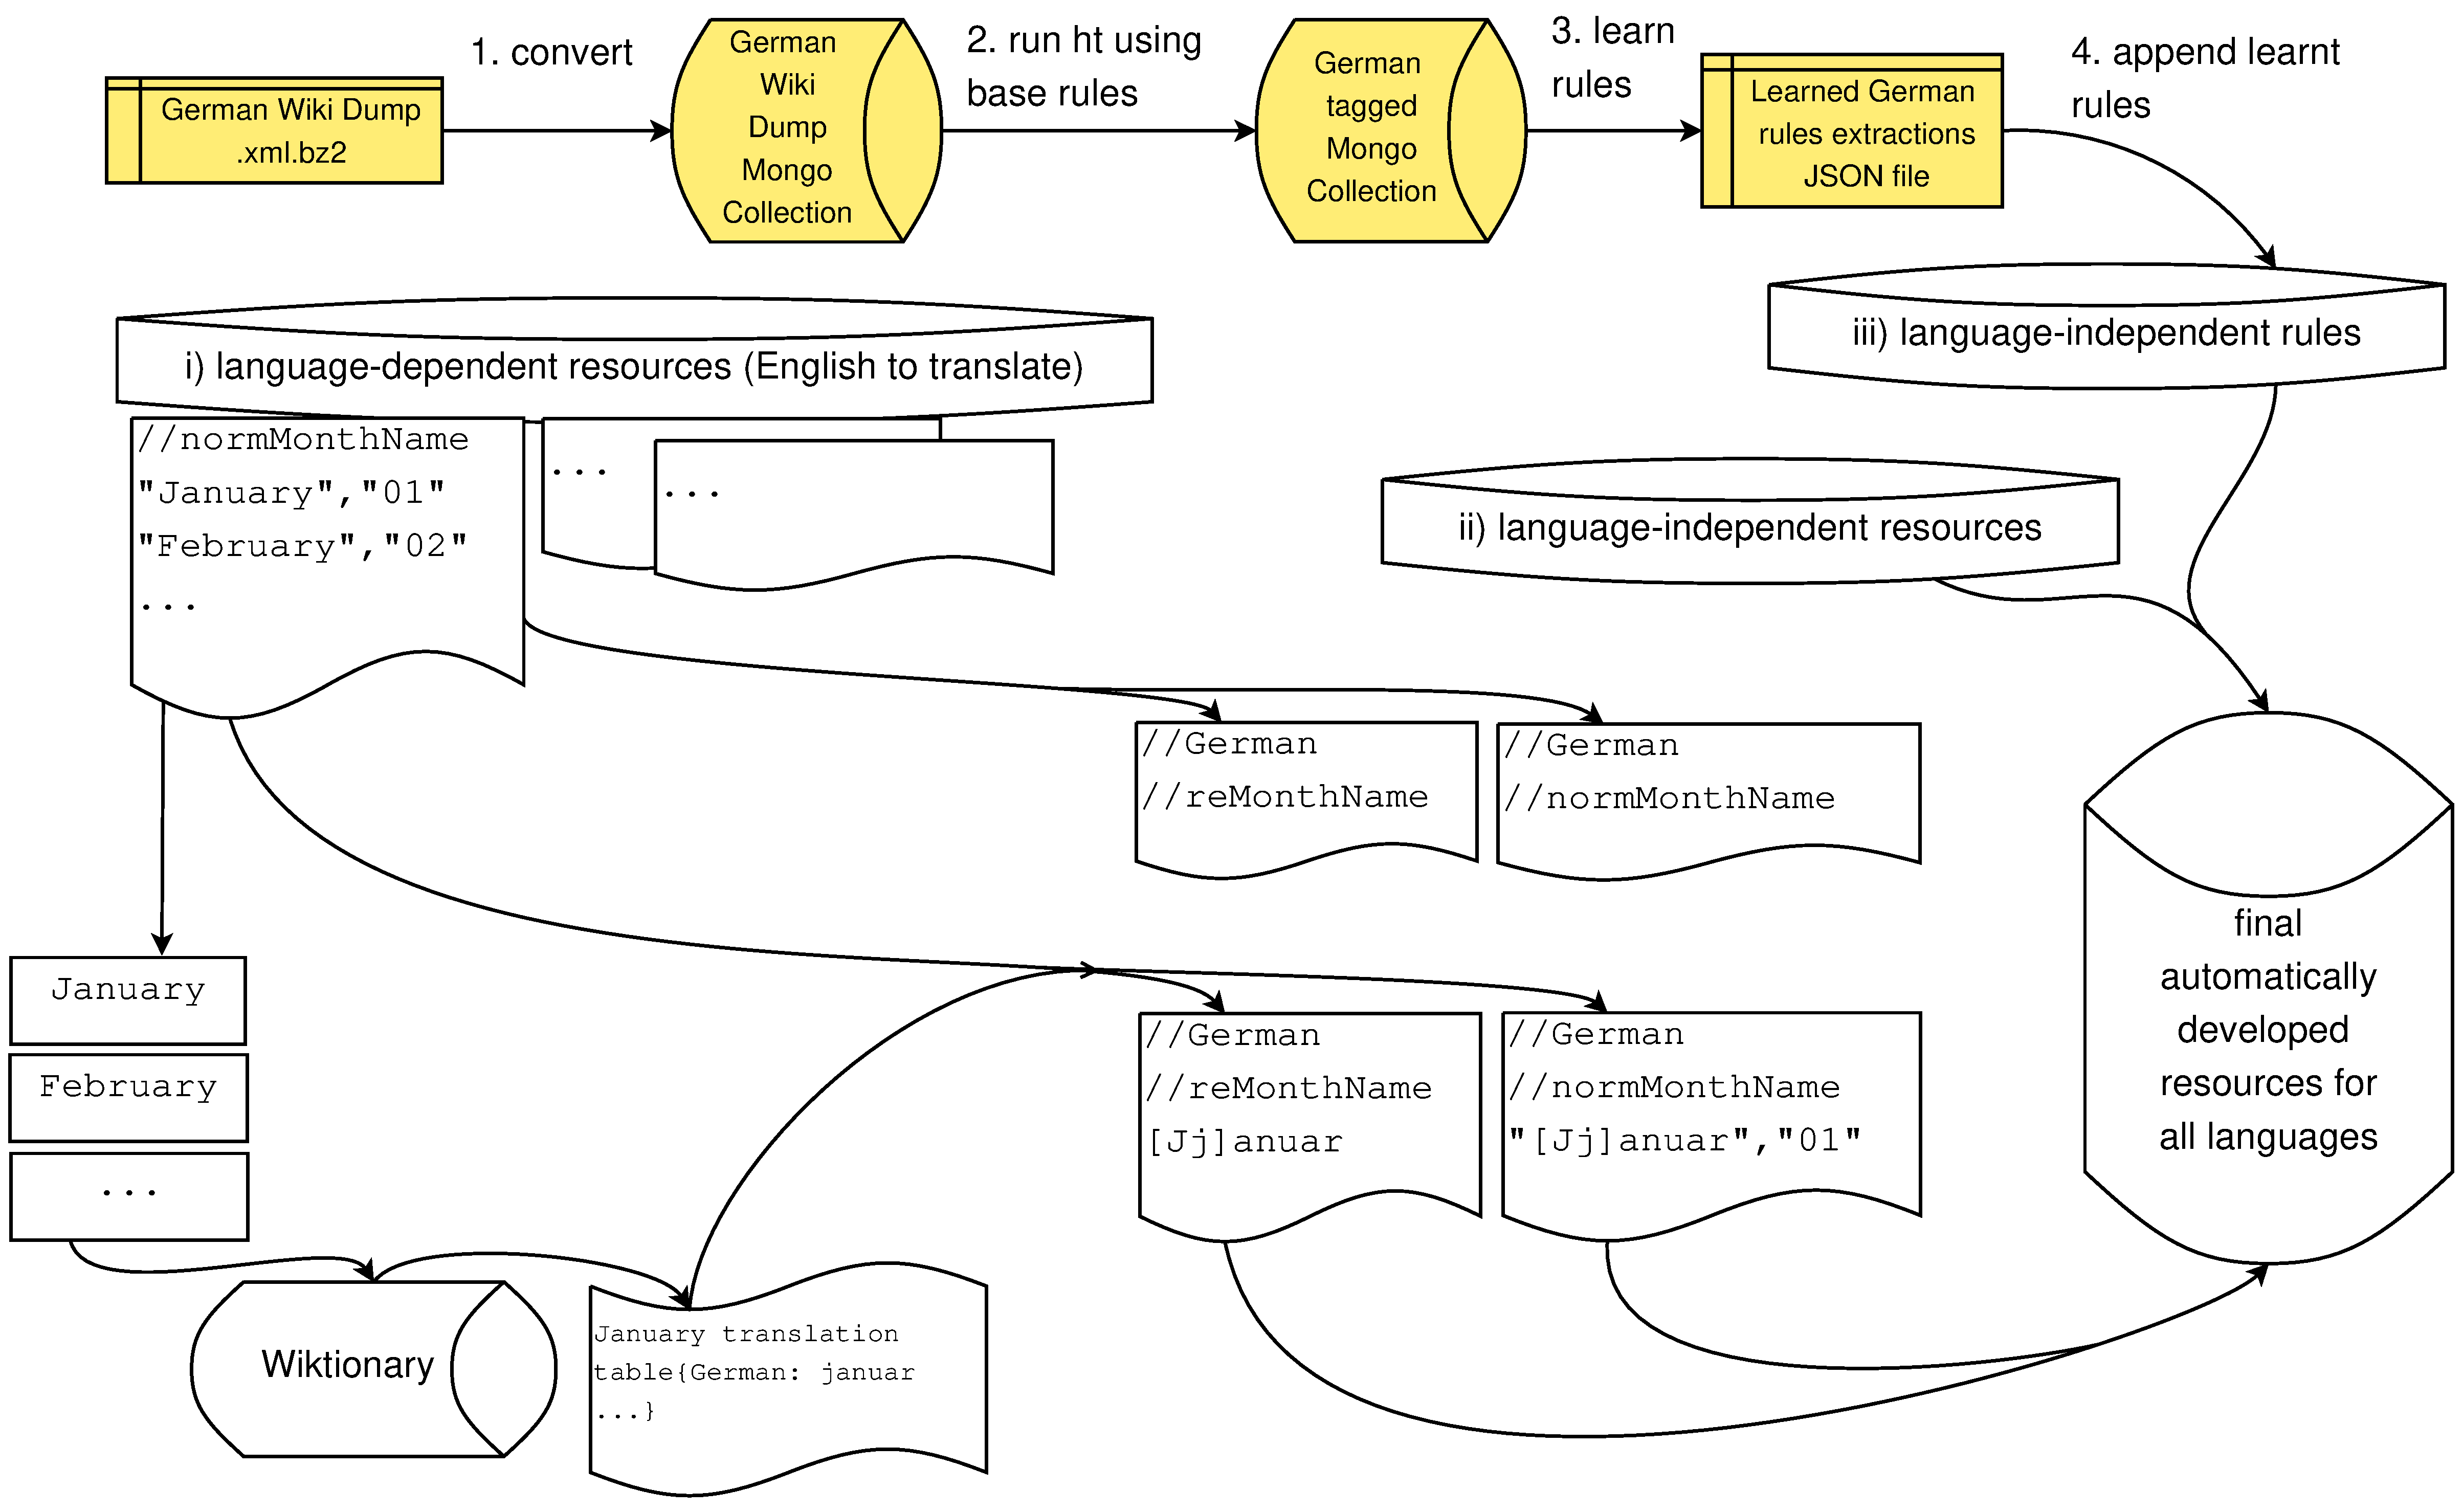
\includegraphics[width=14cm]{Graphics/ht-multilingual-new-3}
	\caption{Overview of Improved Mutlilingual HeidelTime Model - Learning Language-specific Frequent Rules - using Wikipedia.}
	\label{figure:4d}
\end{figure}

\textbf{Learned Rules}\\
In following listing we summarize some of the rules that were learned by our implementation of learning languages specific rules, by analysing respective languages Wikipedia dumps.  \\

\begin{minipage}{\linewidth}
\lstset{caption={Some sample rules learned for different languages.},label={listing:4f}, showspaces=true}
\begin{lstlisting}
// complete date rule for German language
RULENAME="daterules-freq-rule-1",EXTRACTION="%reDayNumber. %reMonthName %reYear4Digit",NORM_VALUE="group(3)-%normMonthName(group(2))-%normDayNumber(group(1))"

// complete date rule for Spanish language
RULENAME="daterules-freq-rule-2",EXTRACTION="%reDayNumber de %reMonthName de %reYear4Digit",NORM_VALUE="group(3)-%normMonthName(group(2))-%normDayNumber(group(1))"

// only year date rule for Finnish language
RULENAME="daterules-freq-rule-3",EXTRACTION="%reYearToken %reYear4Digit",NORM_VALUE="group(2)"

// only year date rule for Finnish language
RULENAME="daterules-freq-rule-4",EXTRACTION="[Vv]uonna %reYear4Digit",NORM_VALUE="group(2)"

// year duration rule for Urdu language 
RULENAME="durationrules-freq-rule-5",EXTRACTION="%reDayNumberWord4Duration %reYearToken",NORM_VALUE="P%normDayNumberWord4Duration(group(1))Y"

// complete date rule for Chinese language
RULENAME="daterules-freq-rule-6",EXTRACTION="%reYear4Digit年%reMonthNumber月%reDayNumber",NORM_VALUE="group(1)-%normMonthNumber(group(2))-%normDayNumber(group(3))"

\end{lstlisting}
\end{minipage}

The first rule, i.e., ``daterules-freq-rule-1" in Listing \ref{listing:4f}, shows the most frequently occurring complete date rule for German language learned by our system. Its extraction part tells that it can extract dates that have reDayNumber followed by dot and space, followed by reMonthName and space, followed by reYear4Digit. For instance, ``20. Januar 2002" can be extracted by this rule. However, there is already a rule (c.f. Listing \ref{listing:4a}) in language independent rules that can extract similar dates.

The second rule, i.e., ``daterules-freq-rule-2" in Listing \ref{listing:4f}, shows the most frequently occurring complete date rule for Spanish language learned by our system. Here the parts of the date are separated by the Spanish word ``de". For instance, ``20 de enero de 2002" can be extracted by this rule. However, such complete dates in Spanish language can already be extracted by one of the rule (c.f. Listing \ref{listing:4a}) in language independent rules. 

The third rule, i.e., ``daterules-freq-rule-3" in Listing \ref{listing:4f}, shows the most frequently occurring only year date rule for Finnish language learned by our system. The rule learnt tells us that in Finnish language year token appears before the year digits. This rule can extract Finnish year only temporal expressions such as the temporal expression ``vuodesta 1971" from the following text\footnote{The Finnish text excerpt is taken from Wikipedia, see \url{https://fi.wikipedia.org/wiki/?curid=30}}.  

\begin{mdframed}[style=MyFrame]
	\raggedright{
		Antti Satuli oli ulkoministeriön palveluksessa \ul{vuodesta 1971} kuolemaansa saakka. Satuli kuoli sairauskohtaukseen ollessaan hiihtomatkalla Lapissa keväällä 2003.
	}
\end{mdframed}

Such a rule that extracts only year temporal expressions is not present in language independent rules; thus, this rule can extract Finnish temporal expressions of year granularity that were not extracted by HeidelTime as of version 2.2.1.

The fourth rule, i.e., ``daterules-freq-rule-4" in Listing \ref{listing:4f}, shows another only year rule learned by our system. This is different from the third rule in that it has the word ``vuonna" itself instead of any pattern name that contains ``vuonna", this is because the word ``vuonna" is not extracted from Wiktionary while making the pattern resources. Such a rule that extract only year temporal expressions is not present in language independent rules; thus, this rule can extract expressions that were not extracted by HeidelTime as of version 2.2.1.

The fifth rule, i.e., ``durationrules-freq-rule-5" in Listing \ref{listing:4f}, shows the a duration rule learned by our system for Urdu language. The rule is reDayNumberWord4Duration followed by space reYearToken. Temporal expressions representing temporal duration in years can be extracted by this rule. For instance, this rule can extract Urdu temporal durations such as \texturdu{پانچ سال}, \texturdu{سات سال}, etc. meaning ``five years" and ``seven years" respectively. However, there is already a similar rule (c.f. rule ``durationrules-freq-rule-1" in Listing \ref{listing:3-lirules}) in language independent rules that can extract such duration temporal expression.

The sixth rule, i.e., ``daterules-freq-rule-6" in Listing \ref{listing:4f}, shows the most frequently occurring complete date rule for Chinese language learned by our system. We can see that reYear4Digit is followed by the Chinese word for year, i.e., 年. Similarly, reMonthNumber is followed by the Chinese word for month, i.e., 月. For instance, this rule can extract Chinese dates such as ``2015年7月29", etc. This rule can extract dates in Chinese that were not extracted using language independent rules as of version 2.2.1 of HeidelTime. 

\textbf{Observations}\\
In general, our system is able to learn simple rules for the different languages (Spanish, German, Finnish, Urdu among others). The simple rules learned are such that some of them are already part of language independent rules. However, we also do learn some rules that are not part of language independent rules. We make following observations about the language specific frequently occurring rules learned by our system. 
\begin{enumerate}[1.]	
	\item Our system was able to learn most frequently occurring order of individual patterns of complete date for various languages such as Spanish, German, Finnish and Chinese.	
	\item Our system was able to learn only year rule for various languages. This rule had two contributing individual patterns, i.e., reYearToken and reYear4Digit, and their correct order along with frequent tokens between them was learned by our system to make the only year rule.
	\item Our system was able to learn only year rule when it had only one contributing individual pattern, i.e., reYear4Digit. The signal word such as `in' was learned and its correct position (before or after) was learned by our system to make this kind of only year rule. For instance, \framebox{\%reYear4Digit \texturdu{میں}} for Urdu language was learned, that translates to \framebox{in \%reYear4Digit} in English. 
\end{enumerate}


%\item 3 iterate over all timexes per document and compare them, based on count - yes 
%-> average number of temporal expressions found per document (old vs new)

%\item 4 iterate over all timexes per document and compare them, based on type - yes
%-> average number of temporal expressions found per type per document (old vs new)

%\item 5 iterate over all timexes per document and compare them, based on normalized value - yes
%-> can draw a graph with normalized years on x-axis and on y axis average number of occurrences in document (old vs new), to find the year that was referred the most

%\item 6 iterate over all timexes per document and compare them, based on abstracted/generalized value (e.g., instead of 2017-11 use YYYY-MM etc.)
%\item 7 iterate over all timexes per document and compare them, based on covered text (i.e., the string which is extracted) -yes

\section{Summary}
In this chapter, we described in detail our contributions to improve the multilingual model of HeidelTime. We started the chapter by discussing the external data sources we use for our work, i.e., Wiktionary, FastText and Wikipedia. In following section, we explained our model, extension of \cite{DBLP:conf/emnlp/StrotgenG15}, that uses Wiktionary to get inflections of patterns while creating the automatically developed resources. Furthermore, we also used FastText, in a separate model, to get inflections. Then, we discussed how we can accommodate unsegmented languages by removing space as delimiter in language independent rules. Finally, we explained our approach to learn frequently occurring temporal patterns as rules. Our system can learn the most frequently occurring order of contributing patterns in the rules and the tokens that separate the patterns. % Implementation / my work

\chapter{Experiments and Evaluation} \label{the-chapter-5}

In this chapter, we discuss the experiments conducted by us to evaluate the tagging performance of HeidelTime using our improved automatically developed resources and the results obtained.
 
\section{Evaluation Approach}
To evaluate our improved automatically developed resources, we use different versions of our created resources. For instance, we use the new resources that only have inflections, the new resources that have both inflections and learned frequently occurring pattern rules in them. Furthermore, we run evaluations on temporally annotated corpora and do analysis on Wikipedia dumps. As explained in Subsection \ref{the-chapter-3-alltc}, only a few languages have temporally annotated corpora, so we will do analysis on Wikipedia dumps for few languages that lack such corpora.

\textbf{Resources Versions}\\
In the following table, we summarize the different versions of HeidelTime resources that we will be evaluating. 

\begin{table}[H]
	\centering
	\rowcolors{1}{}{cream}
	\begin{threeparttable}
		\begin{tabularx}{\linewidth}{||>{\raggedright\arraybackslash}p{.7in} | >{\raggedright\arraybackslash}X |  >{\raggedright\arraybackslash}p{1.2in}||} 
			\hline
			\textbf{Version} & \textbf{About} & \textbf{Reference} \\ [0.5ex] 
			\hline\hline
			2.2.1 & the automatically developed resources with the version 2.2.1 release of HeidelTime (this version disregards inflections)  & Str\"otgen and Gertz in \cite{DBLP:conf/emnlp/StrotgenG15}, and Section \ref{multilingual-ht-model} \\ 
			\hline
			2.x & this version uses wiktionary to get inflections -- and the rules of unsegmented languages do not use space as separator between rePatterns & Subsection \ref{sec4b1} and Section \ref{sec4c} \\ 
			\hline
			2.x-wv & this version uses word vectors to get inflections - (word vectors)& Subsection \ref{sec4b2} \\ 
			\hline
			2.x-afr & same as version 2.x with the addition, i.e., this version has frequently occurring patterns learned as rules - (appended frequent rules) & Section \ref{sec4d} \\ 
			\hline
		\end{tabularx}
%		\begin{tablenotes}
%			\item[1] for unsegmented languages, the rules do not use space as separator between rePatterns
%		\end{tablenotes}
	\end{threeparttable}
	\caption{Summary of different HeidelTime versions for automatically developed resources.}
	\label{table:5a}
\end{table}

\section{Evaluating Using Temporal Corpora}
To evaluate the tagging performance of HeidelTime using the automatically developed resources, we use the following measures, i.e., precision, recall and f1-score. These measures can be better understood with the help of a confusion matrix that describe the decisions of a temporal tagger against the ground truth \cite{DBLP:series/synthesis/2016Strotgen}.

\begin{table}[H]
	\centering
	\begin{threeparttable}
	\begin{tabularx}{380pt}{>{\raggedright\arraybackslash}X|>{\raggedright\arraybackslash}X  >{\raggedright\arraybackslash}X }
		
		\multirow{2}{*}{} & \multicolumn{2}{l}{\textbf{Gold Standard (Ground Truth)}} \\
		\textbf{System Prediction}	 & Positive & Negative  \\ 
		\hline
		Positive & TP & FP \\ 
		Negative & FN & TN \\ 
		
	\end{tabularx}
%		\begin{tablenotes}
%			\item[1] for unsegmented languages, the rules do not use space as separator between rePatterns
%		\end{tablenotes}
	\end{threeparttable}
	\caption{Confusion matrix for temporal tagger decisions.}
	\label{table:5b}
\end{table}

The Table \ref{table:5b}, summarizes the four classes that each of the decision of a temporal tagger can be fall in. 
\begin{itemize}
	\item True Positive (TP): identified as a positive by the system, and was also positive in the gold standard (correct decision)
	\item False Positive (FP): identified as a positive by the system, but was negative in the gold standard (incorrect decision)
	\item False Negative (FN): identified as a negative by the system, but was positive in the gold standard (incorrect decision)
	\item True Negative (TN): identified as a negative by the system, and was also negative in gold standard (correct decision)
\end{itemize}

\subsection{Evaluation Measures}
The three frequently used measures for evaluating performance of temporal taggers on temporally annotated corpara are: precision, recall and f1-score. 

\textbf{Precision}\\
For the task of temporal expression extraction, precision would be the fraction of correctly extracted temporal expressions out of all extracted temporal expressions. And for the task of temporal expression normalization, precision would be the fraction of correctly normalized temporal expressions out of all normalized temporal expressions. It is calcuated using the following formula:
$$P = \frac{TP}{TP+FP}$$
It is evident that a system can achieve higher precision by extracting a few temporal expressions only. For instance, if corpora has 100 true temporal expressions, and system extracts 10 expressions and 9 of them are indeed temporal expressions, the precision of system will be $\frac{9}{10} = 0.9$. As we can see from this example, that a system can achieve high precision even if it extract a small part of all temporal expressions in a corpora (only 9 out of 100 in this example). So it is not good to only rely on precision to evaluate a system. 

\textbf{Recall}\\
For the task of temporal expression extraction, recall would be the fraction of correctly extracted temporal expressions out of all true temporal expressions. And for the task of temporal expression normalization, recall would be the fraction of correctly normalized temporal expressions out of all true normalized temporal expressions. It is calculated using the following formula:
$$R = \frac{TP}{TP+FN}$$
It is evident that a system can achieve higher recall by extracting all expressions in corpora as temporal expressions. Recall is a non-decreasing function of the number of expressions extracted or normalized. So it is not good to only rely on recall to evaluate a system. 

%\begin{table}[H]
%	\centering
%	\rowcolors{1}{}{cream}
%	\begin{threeparttable}
%		\begin{tabularx}{\linewidth}{||>{\raggedright\arraybackslash}p{1.6in} | >{\raggedright\arraybackslash}X |  >{\raggedright\arraybackslash}X||} 
%			\hline
%			\textbf{-} & \textbf{Is Temporal Expression} & \textbf{Is Not Temporal Expression} \\ [0.5ex] 
%			\hline\hline
%			Extracted & tp  & fp \\ 
%			\hline
%			Not Extracted & fn & tn \\ 
%			\hline
%		\end{tabularx}
%		%		\begin{tablenotes}
%		%			\item[1] for unsegmented languages, the rules do not use space as separator between rePatterns
%		%		\end{tablenotes}
%	\end{threeparttable}
%	\caption{Decisions of a temporal tagger - confusion matrix.}
%	\label{table:5b}
%\end{table}

\textbf{F\textsubscript{1} score}\\
F\textsubscript{1} score combines both precision and recall to balance out their shortcomings. It is given by the following formula: 
$$F_1 = \frac{2\times P\times R}{P+R}$$ 
This measure can be seen as a harmonic mean of precision and recall. F\textsubscript{1} score can be seen as a balancing measure which balances out the skew in our system results if we rely on only precision or only recall.

\subsection{Strict and Relaxed Matching}
As temporal expressions may consist of more than one consecutive tokens, so there is a possibility that an extracted temporal expression might overlap with another extracted temporal expression \cite{DBLP:series/synthesis/2016Strotgen}. Moreover, such temporal expressions might be extracted completely or some part of them might be extracted. Due to this temporal taggers can be evaluated using either strict matching or relaxed matching. We demonstrate this with the following example:

\begin{mdframed}[style=MyFrame]
	\raggedright{
		\textbf{Gold Standard}\\
		The car that was lost on <TIMEX3>\underline{1st June}</TIMEX3> was found <TIMEX3>\underline{about three weeks later}</TIMEX3>. 
		
		\textbf{Annotated by a tagger}\\
		The car that was lost on <TIMEX3>\underline{1st June}</TIMEX3> was found about <TIMEX3>\underline{three weeks later}</TIMEX3>. 
	}
\end{mdframed}

In above example, we can see that the gold standard has two temporal expressions, i.e.,  ``1st June" and ``about three weeks later", and a tagger tags the first temporal expression completely and the second one partially. If we evaluate the tagger's extraction performance using strict matching, there is 1 true positive (``1st June"), 1 false positive (``three weeks later") and 1 false negative (``about three weeks later"). However, using relaxed matching there are 2 true positives (``1st June" and ``three weeks later"). It is to be noted that in relaxed matching the second temporal expressions that was annotated by the tagger, was considered a true positive because it overlapped with its annotation in the gold standard. For a detailed discussion about strict and relaxed matching and issues in evaluating temporal taggers, we refer the reader to the book \cite{DBLP:series/synthesis/2016Strotgen}.

The organizers of TempEval-3, consider \textit{value f1-score with relaxed matching} as the most informative measure to evaluate temporal taggers. That is, for extraction consider relaxed matching, and for normalization consider correct value normalization. 

\subsection{Results and Discussion}
The temporal corpora we will be evaluating on are summarized in the Subsection \ref{tactac}. Following, we disucss the evaluation results. 

\textbf{The AncientTimes Corpus - Several Languages}\\
In the following table, we summarize the evaluation results for AncientTimes corpus. 

\begin{table}[H]
	\centering
%	\rowcolors{1}{}{cream}
	\begin{threeparttable}
		\begin{tabularx}{\linewidth}{|| >{\raggedright\arraybackslash}p{.5in} >{\raggedright\arraybackslash}p{.5in} | X X X | X X X | X X ||} 
			\hline
			\multicolumn{2}{||c}{\multirow{2}{*}{}} & \multicolumn{3}{c}{Strict Extraction} & \multicolumn{3}{c}{Relaxed Extraction} & \multicolumn{2}{c||}{Attribute} \\ [0.5ex] 
%			\hline
			\textbf{corpus} & \textbf{version} & \textbf{P} & \textbf{R} & \textbf{F1} & \textbf{P} & \textbf{R} & \textbf{F1} & \textbf{value F1} & \textbf{type F1}\\ 
			\hline\hline
			
			\multirow{3}{\linewidth}{\scriptsize{Ancient Times German}} & 2.2.1 & 76.64 & 45.05 & 56.75 & 100.0 & 58.79 & 74.05 & 67.82 & 73.36 \\ 
			\cline{2-10} & 2.x & 75.0 & 47.8 & 58.39 & 100.0 & 63.74 & 77.85 & 67.79 & 73.15 \\
			\cline{2-10} & 2.x-wv & 61.9 & 7.14 & 12.81 & 100.0 & 11.54 & 20.69 & 11.82 & 20.69 \\  
			\cline{2-10} & 2.x-afr & 74.36 & 47.8 & 58.19 & 100.0 & 64.29 & \textbf{78.26} & \textbf{68.23} & 73.58 \\ 
			\hline\hline
			
			\multirow{3}{\linewidth}{\scriptsize{Ancient Times Spanish}} & 2.2.1 & 23.61 & 8.06 & 12.01 & 58.33 & 19.91 & 29.68 & 16.25 & 28.98 \\ 
			\cline{2-10} & 2.x & 23.61 & 8.06 & 12.01 & 58.33 & 19.91 & 29.68 & \textbf{16.25} & 28.98 \\ 
			\cline{2-10} & 2.x-wv & 27.45 & 6.64 & 10.69 & 50.98 & 12.32 & 19.85 & 16.03 & 19.85 \\  
			\cline{2-10} & 2.x-afr & 22.67 & 8.06 & 11.89 & 60.0 & 21.33 & \textbf{31.47} & 16.08 & 30.77 \\ 
			\hline\hline
			
			\multirow{3}{\linewidth}{\scriptsize{Ancient Times French}} & 2.2.1 & 59.52 & 26.32 & 36.5 & 99.21 & 43.86 & 60.83 & 53.53 & 60.83 \\ 
			\cline{2-10} & 2.x & 59.52 & 26.32 & 36.5 & 99.21 & 43.86 & \textbf{60.83} & \textbf{53.53} & 60.83 \\
			\cline{2-10} & 2.x-wv & 70.45 & 10.88 & 18.84 & 100.0 & 15.44 & 26.75 & 20.67 & 24.92 \\
			\cline{2-10} & 2.x-afr & 59.52 & 26.32 & 36.5 & 99.21 & 43.86 & 60.83 & 50.61 & 58.39 \\
			\hline\hline
			
			\multirow{3}{\linewidth}{\scriptsize{Ancient Times Dutch}} & 2.2.1 & 62.79 & 21.6 & 32.14 & 90.7 & 31.2 & 46.43 & 22.62 & 42.86 \\ 
			\cline{2-10} & 2.x & 62.79 & 21.6 & 32.14 & 90.7 & 31.2 & 46.43 & 22.62 & 42.86 \\
			\cline{2-10} & 2.x-wv & 53.85 & 11.2 & 18.54 & 84.62 & 17.6 & 29.14 & 22.52 & 27.81 \\
			\cline{2-10} & 2.x-afr & 62.79 & 21.6 & 32.14 & 90.7 & 31.2 & \textbf{46.43} & \textbf{22.62} & 42.86 \\ 
			\hline\hline
			
			\multirow{3}{\linewidth}{\scriptsize{Ancient Times Italian}} & 2.2.1 & 68.99 & 38.86 & 49.72 & 96.9 & 54.59 & 69.83 & 57.54 & 69.27 \\ 
			\cline{2-10} & 2.x & 68.99 & 38.86 & 49.72 & 96.9 & 54.59 & 69.83 & 57.54 & 69.27 \\
			\cline{2-10} & 2.x-wv & 67.39 & 13.54 & 22.55 & 95.65 & 19.21 & 32.0 & 20.36 & 31.27 \\
			\cline{2-10} & 2.x-afr & 64.49 & 38.86 & 48.5 & 97.1 & 58.52 & \textbf{73.02} & \textbf{58.86} & 71.93 \\ 
			\hline\hline
			
			\multirow{3}{\linewidth}{\scriptsize{Ancient Times Vietnamese}} & 2.2.1 & 2.38 & 0.86 & 1.27 & 69.05 & 25.0 & 36.71 & 5.06 & 18.99 \\ 
			\cline{2-10} & 2.x & 2.38 & 0.86 & 1.27 & 69.05 & 25.0 & \textbf{36.71} & 1.27 & 18.99 \\ 
			\cline{2-10} & 2.x-wv & 2.94 & 0.86 & 1.33 & 76.47 & 22.41 & 34.67 & \textbf{6.67} & 6.67 \\
			\cline{2-10} & 2.x-afr & 2.33 & 0.86 & 1.26 & 67.44 & 25.0 & 36.48 & 6.29 & 16.35 \\ 
			\hline\hline
			
			\multirow{3}{\linewidth}{\scriptsize{Ancient Times Arabic}} & 2.2.1 & 12.5 & 0.99 & 1.83 & 62.5 & 4.95 & \textbf{9.17} & \textbf{3.67} & 7.34 \\ 
			\cline{2-10} & 2.x &  0.0 & 0.0 & 0.0 & 50.0 & 1.98 & 3.81 & 1.9 & 3.81 \\ 
			\cline{2-10} & 2.x-wv & 0.0 & 0.0 & 0.0 & 16.67 & 1.98 & 3.54 & 0.0 & 3.54 \\
			\cline{2-10} & 2.x-afr &  0.0 & 0.0 & 0.0 & 50.0 & 1.98 & 3.81 & 1.9 & 3.81 \\  
			\hline
				
		\end{tabularx}
		%		\begin{tablenotes}
		%			\item[1] for unsegmented languages, the rules do not use space as separator between rePatterns
		%		\end{tablenotes}
	\end{threeparttable}
	\caption{Evaluation results for AncientTimes corpora.}
	\label{table:5-results-at}
\end{table}

\clearpage 

The Table \ref{table:5-results-at}, for AncientTimes corpus, shows that there wasn't an improvement over the version 2.2.1 resources when using the version 2.x resources for all languages except for the German language for which the F1 score for relaxed extraction increased from 74.05 to 77.85. The reason for not seeing any improvements when using 2.x version resources is that they only cater the morphologically rich languages and unsegmented languages. And the AncientTimes corpus does not has such languages so we did not see an improvement over 2.2.1 resources. While using the 2.x-wv version resources, made using Yandex Translate and FastText word vectors, the results got worse for all the languages in AncientTimes corpus. However, for version 2.x-afr resources, we see some improvement for relaxed extraction scores for almost all the languages. This was due to the frequently occurring patterns being learned as HeidelTime rules. 

For instance, for German language, relaxed extraction F1 score increased to 78.26 when using 2.x-afr resources versus 74.05 for 2.2.1 resources.  Similarly, we see an increase in relaxed extraction F1 scores for Spanish and Italian. For instance, one temporal expression for Italian language that was not found by version 2.x but found by version 2.x-afr was ``anno seguente", that translates\footnote{using Google Translate} to ``following year", by a newly learned rule having extraction part: \framebox{\%reYearToken \%reThisNextLast}. However, for languages French and Dutch the relaxed extraction F1 scores remained same. 

We also noted that for French language, the F1 score of value normalization dropped from 53.53 using 2.2.1 resources to 50.61 using 2.x-afr resources. This was due to a date rule learned, that caught temporal expressions that were previously correctly caught by a duration rule. One such French temporal expression ``trois mois", that translates to ``three months", was correctly extracted by the duration type rule: \framebox{\%reDayNumberWord4Duration \%reUnit} using version 2.2.1 resources. However, a similar date rule: \framebox{\%reDayNumberWordTh \%reUnit4Duration}, to extract expressions such as ``third month", caught this temporal expression using version 2.x-afr resources; thus, leading to lower type and value normalization scores. 

%This was because in the reDayNumberWordTh resource file for French, there are two translations for ``third", i.e., troisième and trois.

 
%\textcolor{violet}{timebank results...}
%\begin{table}[H]
%	\centering
%	%	\rowcolors{1}{}{cream}
%	\begin{threeparttable}
%		\begin{tabularx}{\linewidth}{|| >{\raggedright\arraybackslash}p{.5in} >{\raggedright\arraybackslash}p{.5in} | X X X | X X X | X X ||} 
%			\hline
%			\multicolumn{2}{||c}{\multirow{2}{*}{}} & \multicolumn{3}{c}{Strict Extraction} & \multicolumn{3}{c}{Relaxed Extraction} & \multicolumn{2}{c||}{Attribute} \\ [0.5ex] 
%			%			\hline
%			\textbf{corpus} & \textbf{version} & \textbf{P} & \textbf{R} & \textbf{F1} & \textbf{P} & \textbf{R} & \textbf{F1} & \textbf{value F1} & \textbf{type F1}\\ 
%			\hline\hline
%			
%			\multirow{3}{\linewidth}{\scriptsize{TimeBank Portuguese}} & 2.2.1 & 75.53 & 48.97 & 59.41 & 91.49 & 59.31 & 71.97 & 59.41 & 66.11 \\ 
%			\cline{2-10} & 2.x & 75.27 & 48.28 & 58.82 & 91.4 & 58.62 & 71.43 & 58.82 & 65.55 \\ 
%			\cline{2-10} & 2.x-afr & ? & ? & ? & ? & ? & ? & ? & ? \\ 
%			\hline
%			
%			
%			\multirow{3}{\linewidth}{\scriptsize{French TimeBank 1.1}} & 2.2.1 & 63.64 & 44.47 & 52.35 & 87.54 & 61.18 & 72.02 & 56.23 & 68.7 \\ 
%			\cline{2-10} & 2.x & 63.76 & 44.71 & 52.56 & 87.58 & 61.41 & 72.2 & 56.15 & 68.88 \\ 
%			\cline{2-10} & 2.x-afr & ? & ? & ? & ? & ? & ? & ? & ? \\ 
%			\hline
%			
%		\end{tabularx}
%		%		\begin{tablenotes}
%		%			\item[1] for unsegmented languages, the rules do not use space as separator between rePatterns
%		%		\end{tablenotes}
%	\end{threeparttable}
%	\caption{Evaluation results for TimeBank corpus.}
%	\label{table:5-results-tb}
%\end{table}

\clearpage
\textbf{WikiWarsDE Corpus - German}\\
Now we move to the WikiWarsDE corpus for German language. The following table summarizes the evaluation results for WikiWarsDE corpus. 
\begin{table}[H]
	\centering
	%	\rowcolors{1}{}{cream}
	\begin{threeparttable}
		\begin{tabularx}{360pt}{|| >{\raggedright\arraybackslash}p{.5in} >{\raggedright\arraybackslash}p{.5in} | X X X | X X X ||} 
			\hline
			\multicolumn{2}{||c}{\multirow{2}{*}{}} & \multicolumn{3}{c}{Relaxed Extraction} & \multicolumn{3}{c||}{Full task\tnote{1}} \\ [0.5ex] 
			%			\hline
			\textbf{corpus} & \textbf{version} & \textbf{P} & \textbf{R} & \textbf{F1} & \textbf{P} & \textbf{R} & \textbf{F1} \\ 
			\hline\hline
			
			\multirow{3}{\linewidth}{\scriptsize{WikiWars DE}} & 2.2.1 & 98.4 & 65.0 & 78.3 & 75.7 & 50.0 & 60.2 \\ 
			\cline{2-8} & 2.x & 98.2 & 66.3 & 79.1 & 76.2 & 51.4 & 61.4 \\ 
			\cline{2-8} & 2.x-wv & 98.8 & 22.2 & 36.3 & 78.4 & 17.6 & 28.8 \\ 
			\cline{2-8} & 2.x-afr & 98.2 & 70.1 & \textbf{81.8} & 77.2 & 55.1 & \textbf{64.3} \\ 
			\hline
						
		\end{tabularx}
				\begin{tablenotes}
					\item[1] scoring full task of temporal tagging; using relaxed matching in extraction and correct normalization of such matches constitutes a true positive.
				\end{tablenotes}
	\end{threeparttable}
	\caption{Evaluation results for WikiWarsDE corpus.}
	\label{table:5-results-ww}
\end{table}

From the evaluation results for WikiWarsDE, in Table \ref{table:5-results-ww}, we see an improvement over version 2.2.1 resources when using version 2.x; for instance, the F1-score for relaxed extraction increased from 78.3 to 79.1, and the F1-score for full task of temporal tagging also increased from 60.2 to 61.4. The version 2.x-wv resources did not get good results, and the scores dropped significantly as compared to version 2.2.1 resources. The version 2.x-afr resources performed the best; for instance, the F1-score for relaxed extraciton increased from 78.3 to 81.8, and the F1-score for full task of temporal tagging also increased from 60.2 to 64.3. 

\textbf{TempEval-2 Corpus - Spanish, Italian, Chinese}\\
The following table summarizes evaluation results for the TempEval-2 corpora, for languages Spanish, Italian and Chinese. 
\begin{table}[H]
	\centering
	%	\rowcolors{1}{}{cream}
	\begin{threeparttable}
		\begin{tabularx}{300pt}{|| >{\raggedright\arraybackslash}p{.5in} >{\raggedright\arraybackslash}p{.5in} | X X X | X X ||} 
			\hline
			\multicolumn{2}{||c}{\multirow{2}{*}{}} & \multicolumn{3}{c}{Extraction} & \multicolumn{2}{c||}{Attribute} \\ [0.5ex] 
			%			\hline
			\textbf{corpus} & \textbf{version} & \textbf{P} & \textbf{R} & \textbf{F1} & \textbf{value} & \textbf{type} \\ 
			\hline\hline
			
			\multirow{3}{\linewidth}{\scriptsize{TempEval-2 Spanish}} & 2.2.1 & 97.5 & 41.1 & 57.8 & 94.0 & 100.0  \\ 
			\cline{2-7} & 2.x & 97.5 & 41.1 & 57.8 & 94.0 & 100.0  \\
			\cline{2-7} & 2.x-wv & 95.7 & 23.7 & 38.0 & 92.0 & 100.0  \\  
			\cline{2-7} & 2.x-afr & 97.6 & 42.1 & \textbf{58.8} & \textbf{94.0} & 100.0  \\ 
			\hline\hline
			
			\multirow{3}{\linewidth}{\scriptsize{TempEval-2 Italian}} & 2.2.1 & 93.6 & 41.5 & 57.5 & 97.0 & 100.0 \\ 
			\cline{2-7} & 2.x & 93.6 & 41.5 & 57.5 & 97.0 & 100.0  \\ 
			\cline{2-7} & 2.x-wv & 93.5 & 27.4 & 42.3 & 96.0 & 100.0  \\  
			\cline{2-7} & 2.x-afr & 93.9 & 43.4 & \textbf{59.4} & \textbf{97.0} & 100.0  \\ 
			\hline\hline
			
			\multirow{3}{\linewidth}{\scriptsize{TempEval-2 Chinese Training}} & 2.2.1 & 100.0 & 9.7 & 17.7 & 42.0 & 94.0  \\ 
			\cline{2-7} & 2.x & 69.8 & 20.6 & 31.8 & 54.0 & 77.0  \\ 
			\cline{2-7} & 2.x-wv & 82.1 & 12.7 & 22.0 & 49.0 & 92.0  \\  
			\cline{2-7} & 2.x-afr & 69.8 & 20.6 & \textbf{31.8} & \textbf{54.0} & 77.0  \\
			\hline\hline
			
			\multirow{3}{\linewidth}{\scriptsize{TempEval-2 Chinese Test}} & 2.2.1 & 96.8 & 9.1 & 16.7 & 22.0 & 100.0  \\ 
			\cline{2-7} & 2.x & 72.4 & 19.2 & 30.4 & 32.0 & 63.0\\ 
			\cline{2-7} & 2.x-wv & 96.6 & 8.5 & 15.7 & 31.0 & 92.0 \\
			\cline{2-7} & 2.x-afr & 72.4 & 19.2 & \textbf{30.4} & \textbf{32.0} & 63.0 \\
			\hline\hline
			
			\multirow{3}{\linewidth}{\scriptsize{TempEval-2 Chinese Training CLEAN}} & 2.2.1 & 94.6 & 11.2 & 20.0 & 42.0 & 94.0  \\ 
			\cline{2-7} & 2.x & 60.1 & 21.6 & 31.8 & 55.0 & 78.0  \\ 
			\cline{2-7} & 2.x-afr & 60.1 & 21.6 & \textbf{31.8} & \textbf{55.0} & 78.0  \\
			\hline\hline
			
			\multirow{3}{\linewidth}{\scriptsize{TempEval-2 Chinese Test CLEAN}} & 2.2.1 & 71.0 & 10.6 & 18.4 & 31.0 & 100.0  \\ 
			\cline{2-7} & 2.x & 47.1 & 19.7 & 27.8 & 47.0 & 68.0 \\ 
			\cline{2-7} & 2.x-afr & 47.1 & 19.7 & \textbf{27.8} & \textbf{47.0} & 68.0 \\
			\hline\hline
			
			\multirow{3}{\linewidth}{\scriptsize{TempEval-2 Chinese Training IMPR.}} & 2.2.1 & 100.0 & 9.7 & 17.7 & 43.0 & 94.0  \\ 
			\cline{2-7} & 2.x & 71.6 & 21.2 & 32.7 & 54.0 & 76.0 \\ 
			\cline{2-7} & 2.x-afr & 71.6 & 21.2 & \textbf{32.7} & \textbf{54.0} & 76.0 \\
			\hline\hline
			
			\multirow{3}{\linewidth}{\scriptsize{TempEval-2 Chinese Test IMPR.}} & 2.2.1 & 100 & 9.5 & 17.3 & 44.0 & 100.0 \\ 
			\cline{2-7} & 2.x & 71.3 & 18.9 & 29.9 & 44.0 & 67.0 \\ 
			\cline{2-7} & 2.x-afr & 71.3 & 18.9 & \textbf{29.9} & \textbf{44.0} & 67.0 \\
			\hline
		\end{tabularx}
%		\begin{tablenotes}
%			\item[1] scoring full task of temporal tagging; using relaxed matching in extraction and correct normalization of such matches constitutes a true positive.
%		\end{tablenotes}
	\end{threeparttable}
	\caption{Evaluation results for TempEval-2 corpora.}
	\label{table:5-results-tempeval2}
\end{table}
\clearpage

The evaluation results, in Table \ref{table:5-results-tempeval2}, show no improvement when using version 2.x resources over version 2.2.1 resources for Spanish and Italian languages. However, we see improvement in F1 scores for extraction when using version 2.x-afr resources over version 2.2.1 resources; for instance, for Spanish language the relaxed extraction F1-score was 57.8 when using version 2.x resources, same as version 2.2.1 resources. And the relaxed extraction F1-score increased from 57.8 to 58.8 when using version 2.x-afr resources for Spanish language. The scores for version 2.x-wv resources dropped as compared to version 2.2.1 for all the languages. 

For Chinese language we can see improvement for both the tasks of extraction and normalization when using version 2.x resources over 2.2.1 resources. For instance, for TempEval-2 Chinese Training corpus, the relaxed extraction F1-score was 31.8 when using version 2.x resources as compared to 17.7 when using version 2.2.1 resources. The better results for Chinese language when using version 2.x resources can be attributed to the modified rules for unsegmented languages, that had spaces removed from the language independent rules. We also noted that version 2.x-afr resources had identical scores to the version 2.x resources for Chinese corpora, i.e., frequently occurring temporal patterns learned as rules, for Chinese language, did not improve the results for the TempEval-2 corpora.

\textbf{Further corpora - several languages}\\
In the following table, we summarize evaluation results for some more corpora, using TempEval-3 evaluation style. 
\begin{table}[H]
	\centering
	%	\rowcolors{1}{}{cream}
	\begin{threeparttable}
		\begin{tabularx}{\linewidth}{|| >{\raggedright\arraybackslash}p{.5in} >{\raggedright\arraybackslash}p{.5in} | X X X | X X X | X X ||} 
			\hline
			\multicolumn{2}{||c}{\multirow{2}{*}{}} & \multicolumn{3}{c}{Strict Extraction} & \multicolumn{3}{c}{Relaxed Extraction} & \multicolumn{2}{c||}{Attribute} \\ [0.5ex] 
			%			\hline
			\textbf{corpus} & \textbf{version} & \textbf{P} & \textbf{R} & \textbf{F1} & \textbf{P} & \textbf{R} & \textbf{F1} & \textbf{value F1} & \textbf{type F1}\\ 
			\hline\hline
			
			%			\multirow{3}{\linewidth}{\scriptsize{WikiWars DE}} & 2.2.1 & 0.851 & 0.562 & 0.677 & 0.984 & 0.650 & 0.783 & 0.769 & - \\ 
			%			\cline{2-10} & 2.x & 0.848 & 0.572 & 0.683 & 0.982 & 0.663 & 0.791 & 0.776 & - \\ 
			%			\cline{2-10} & 2.x-afr & 0.844 & 0.592 & 0.696 & 0.982 & 0.688 & 0.809 & 0.799 & - \\ 
			%			\hline
						
			\multirow{3}{\linewidth}{\scriptsize{TimeBank Portuguese}} & 2.2.1 & 75.53 & 48.97 & 59.41 & 91.49 & 59.31 & 71.97 & 59.41 & 66.11 \\ 
			\cline{2-10} & 2.x & 75.27 & 48.28 & 58.82 & 91.4 & 58.62 & 71.43 & 58.82 & 65.55 \\ 
			\cline{2-10} & 2.x-wv & 75.32 & 40.0 & 52.25 & 90.91 & 48.28 & 63.06 & 56.76 & 60.36 \\ 
			\cline{2-10} & 2.x-afr & 73.2 & 48.97 & 58.68 & 91.75 & 61.38 & \textbf{73.55} & \textbf{61.16} & 66.94 \\ 
			\hline\hline
			
			
			\multirow{3}{\linewidth}{\scriptsize{TimeBank French 1.1}} & 2.2.1 & 63.64 & 44.47 & 52.35 & 87.54 & 61.18 & 72.02 & \textbf{56.23} & 68.7 \\ 
			\cline{2-10} & 2.x & 63.76 & 44.71 & 52.56 & 87.58 & 61.41 & 72.2 & 56.15 & 68.88 \\ 
			\cline{2-10} & 2.x-wv & 66.48 & 28.47 & 39.87 & 91.76 & 39.29 & 55.02 & 37.89 & 48.76 \\
			\cline{2-10} & 2.x-afr & 62.5 & 44.71 & 52.13 & 87.83 & 62.82 & \textbf{73.25} & 55.69 & 68.59 \\ 
			\hline\hline
			
			\multirow{3}{\linewidth}{\scriptsize{TempEval-2 Italian Training\tnote{1}}} & 2.2.1 & 58.42 & 22.56 & 32.55 & 86.14 & 33.27 & 48.0 & 39.45 & 47.45 \\ 
			\cline{2-10} & 2.x & 58.42 & 22.56 & 32.55 & 86.14 & 33.27 & 48.0 & 39.45 & 47.45 \\
			\cline{2-10} & 2.x-wv & 61.27 & 20.27 & 30.46 & 89.6 & 29.64 & 44.54 & 35.63 & 42.24 \\
			\cline{2-10} & 2.x-afr & 53.64 & 22.56 & 31.76 & 87.27 & 36.71 & \textbf{51.68} & \textbf{42.8} & 51.14 \\ 
			\hline\hline
			
			\multirow{3}{\linewidth}{\scriptsize{TempEval-2 Italian Test\tnote{1}}} & 2.2.1 & 80.33 & 38.89 & 52.41 & 95.08 & 46.03 & 62.03 & 59.89 & 62.03 \\ 
			\cline{2-10} & 2.x & 80.33 & 38.89 & 52.41 & 95.08 & 46.03 & 62.03 & 59.89 & 62.03 \\ 
			\cline{2-10} & 2.x-wv & 80.0 & 28.57 & 42.11 & 95.56 & 34.13 & 50.29 & 47.95 & 50.29 \\
			\cline{2-10} & 2.x-afr & 79.37 & 39.68 & 52.91 & 95.24 & 47.62 & \textbf{63.49} & \textbf{61.38} & 63.49 \\ 
			\hline\hline
			
			\multirow{3}{\linewidth}{\scriptsize{TempEval-3 trainT3 Spanish}} & 2.2.1 & 56.94 & 32.63 & 41.49 & 92.98 & 53.29 & 67.75 & \textbf{54.85} & 63.45 \\ 
			\cline{2-10} & 2.x & 56.94 & 32.63 & 41.49 & 92.98 & 53.29 & 67.75 & 54.85 & 63.45 \\ 
			\cline{2-10} & 2.x-wv & 60.5 & 26.33 & 36.69 & 93.28 & 40.59 & 56.56 & 45.99 & 52.48 \\
			\cline{2-10} & 2.x-afr & 50.0 & 29.07 & 36.76 & 93.08 & 54.11 & \textbf{68.44} & 54.8 & 64.16 \\ 
			\hline\hline
			
			\multirow{3}{\linewidth}{\scriptsize{Wikiwars VN - Vietnamese}} & 2.2.1 & 61.02 & 32.73 & 42.6 & 84.75 & 45.45 & 59.17 & 44.38 & 47.93 \\ 
			\cline{2-10} & 2.x & 61.02 & 32.73 & 42.6 & 84.75 & 45.45 & 59.17 & 44.38 & 47.93 \\ 
			\cline{2-10} & 2.x-wv & 73.81 & 28.18 & 40.79 & 96.43 & 36.82 & 53.29 & 42.11 & 44.08 \\ 
			\cline{2-10} & 2.x-afr & 70.33 & 58.18 & 63.68 & 89.56 & 74.09 & \textbf{81.09} & \textbf{68.16} & 72.14 \\ 
			
			\hline
		\end{tabularx}
		\begin{tablenotes}
			\item[1] evaluated using TempEval-3 tools
		\end{tablenotes}
	\end{threeparttable}
	\caption{Evaluation results for further corpora - several languages.}
	\label{table:5-results-somemore}
\end{table}
\clearpage

The evaluation results, in Table \ref{table:5-results-somemore}, show minor improvements in F1 score for relaxed extraction when using version 2.x-afr resources over version 2.2.1 resources for Portuguese, French, Italian and Spanish languages. The scores for version 2.x-wv resources were lower than version 2.2.1 resources for all languages corpora. 

In corpus WikiwarsVN, for Vietnamese language, we see a big improvement in scores when using 2.x-afr resources over 2.2.1 or 2.x version resources; for instance, relaxed extraction F1-score jumped to 81.09 (version 2.x-afr) over 59.17 (version 2.2.1), and normalization value F1-score jumped to 68.16 (version 2.x-afr) over 44.38 (version 2.2.1). 


\textbf{Morphologically rich languages corpora - Croatian and Estonian}\\
In the following table, we summarize evaluation results for the morphologically rich languages corpora.
\begin{table}[H]
	\centering
	%	\rowcolors{1}{}{cream}
	\begin{threeparttable}
		\begin{tabularx}{\linewidth}{|| >{\raggedright\arraybackslash}p{.5in} >{\raggedright\arraybackslash}p{.5in} | X X X | X X X | X X ||} 
			\hline
			\multicolumn{2}{||c}{\multirow{2}{*}{}} & \multicolumn{3}{c}{Strict Extraction} & \multicolumn{3}{c}{Relaxed Extraction} & \multicolumn{2}{c||}{Attribute} \\ [0.5ex] 
			%			\hline
			\textbf{corpus} & \textbf{version} & \textbf{P} & \textbf{R} & \textbf{F1} & \textbf{P} & \textbf{R} & \textbf{F1} & \textbf{value F1} & \textbf{type F1}\\ 
			\hline\hline
			
			\multirow{3}{\linewidth}{\scriptsize{Wikiwars HR - Croatian}} & 2.2.1 & 38.18 & 3.07 & 5.68 & 87.27 & 7.01 & 12.97 & 10.0 & 12.16 \\ 
			\cline{2-10} & 2.x & 40.47 & 13.8 & 20.58 & 94.86 & 32.34 & 48.23 & 38.43 & 47.47 \\ 
			\cline{2-10} & 2.x-wv & 38.32 & 4.67 & 8.33 & 79.04 & 9.64 & 17.18 & 13.01 & 15.09 \\
			\cline{2-10} & 2.x-afr & 28.42 & 13.94 & 18.71 & 96.13 & 47.15 & \textbf{63.27} & \textbf{54.95} & 62.95 \\ 
			\hline\hline
			
			
			\multirow{3}{\linewidth}{\scriptsize{Annikas-News Estonian\tnote{1}}} & 2.2.1 & 70.73 & 15.1 & 24.89 & 95.12 & 20.31 & 33.48 & 23.18 & 28.33 \\ 
			\cline{2-10} & 2.x & 63.53 & 28.13 & 38.99 & 87.06 & 38.54 & 53.43 & 36.82 & 47.65 \\ 
			\cline{2-10} & 2.x-wv & 69.7 & 11.98 & 20.44 & 90.91 & 15.63 & 26.67 & 17.78 & 21.33 \\
			\cline{2-10} & 2.x-afr & 71.43 & 44.27 & 54.66 & 89.08 & 55.21 & \textbf{68.17} & \textbf{52.73} & 63.02 \\ 
			\hline
			
		\end{tabularx}
		\begin{tablenotes}
			\item[1] Annika Boldt: Estonian Temporal Tagging with HeidelTime, Student Project, Heidelberg University, 2015.
		\end{tablenotes}
	\end{threeparttable}
	\caption{Evaluation results for corpora of morphologically rich languages .}
	\label{table:5-results-somemore-inflection-rich}
\end{table}

The evaluation results, in Table \ref{table:5-results-somemore-inflection-rich}, show big increase in overall extraction and normalization scores when using version 2.x resources over version 2.2.1 for Croatian language; for instance, relaxed extraction F1-score jumped to 48.23 over 12.97. This increase in scores shows that taking inflections into account did help the already present language independent rules a lot to increase the scores this much. The version 2.x-wv resources also see improvements over 2.2.1 version resources (relaxed extraction F1-score of 17.18 over 12.97), albeit they are not as big as the version 2.x. Finally, the version 2.x-afr resources further improve the scores over 2.x version; for instance, relaxed extraction F1-score of 63.27 (version 2.x-afr) over 48.23 (version 2.x); similarly, we see improvement in scores for value normalization.

Furthermore, the results in Table \ref{table:5-results-somemore-inflection-rich}, show big increase in overall extraction and normalization scores using new resources for Estonian language too. For instance, when using version 2.x resources over version 2.2.1 resources, relaxed extraction F1 score increased to 53.43 from 33.48, showing that taking inflections in account hugely improved the baseline scores for Estonian language. The results when using version 2.x-wv show decrease in scores, showing that getting translations from Yandex and  inflections from FastText did not prove beneficial here. However, when using version 2.x-afr resources over version 2.x resources, the scores further improved for Estonian language (relaxed extraction F1-score of 68.17 over 53.43 and value normalization F1-score of 52.73 over 36.82). 



\section{Evaluating Using Multilingual Wikipedia}

In addition to evaluating temporally annotated corpora, we also evaluate performance of our improved resources using Wikipedia dumps for languages that lack such corpora. For instance, we tag MongoDB collection of Wikipedia dump of a certain language using HeidelTime using both current and improved automatically developed resources, and compare. Computing evaluation measures such as precision and recall among others would not be possible while using Wikipedia dumps, as no gold standard temporal annotations are available for these Wikipedia dumps, so we rely on some key metrics that are discussed in following subsection.

\subsection{Evaluation Criteria}
We aim to compare the initial and improved resources for a language using Wikipedia dumps on the following metrics. 

\begin{enumerate}[1.]	
	\item The overall number of temporal expressions extracted.
	\item The overall number of temporal expressions extracted per type.
	\item The percentage of documents that are tagged (contain atleast one temporal expression).
	\item The average number of temporal expressions found per document.
	\item The number of temporal expressions that are normalized to the YYYY-MM-DD format.
\end{enumerate}

\subsection{Results and Discussion}
We summarize the evaluation results on Wikipedia dumps for some chosen languages of the select regions of the world. 

\textbf{Languages of Europe}\\
We summarize the results for some of the languages of Europe, i.e., Polish, Czech and Finnish in the following tables.

\begin{table}[H]
	\centering
	%	\rowcolors{1}{}{cream}
	\begin{threeparttable}
		\begin{tabularx}{\linewidth}{|| >{\raggedright\arraybackslash}p{.5in} >{\raggedright\arraybackslash}p{.6in} | >{\raggedleft\arraybackslash}X | >{\raggedleft\arraybackslash}X >{\raggedleft\arraybackslash}X >{\raggedleft\arraybackslash}X >{\raggedleft\arraybackslash}X ||} 
			\hline
			\multicolumn{2}{||c}{\multirow{2}{*}{}} & \multicolumn{1}{c}{\#1} & \multicolumn{4}{c||}{\#2} \\ [0.5ex] 
			%			\hline
			\textbf{lang.} & \textbf{version} & \textbf{count} & \textbf{date} & \textbf{dur.} & \textbf{time} & \textbf{set} \\ 
			\hline\hline
			
			% DATE DURATION TIME SET
			\multirow{4}{\linewidth}{Polish} & 2.2.1 & \num[group-separator={,}]{237044} & \num[group-separator={,}]{86618} & \num[group-separator={,}]{141274} & \num[group-separator={,}]{9049} & \num[group-separator={,}]{103}  \\ 
			\cline{2-7} & 2.x & \num[group-separator={,}]{604607} & \num[group-separator={,}]{474731} & \num[group-separator={,}]{106090} & \num[group-separator={,}]{23153} & \num[group-separator={,}]{633}  \\ 
			\cline{2-7} & 2.x-wv & \num[group-separator={,}]{300313} & \num[group-separator={,}]{155311} & \num[group-separator={,}]{141779} & \num[group-separator={,}]{3036} & \num[group-separator={,}]{187}  \\ 
			\cline{2-7} & 2.x-afr & \num[group-separator={,}]{795207} & \num[group-separator={,}]{761104} & \num[group-separator={,}]{10317} & \num[group-separator={,}]{23153} & \num[group-separator={,}]{633} \\ 
			\hline\hline
			
			% DATE DURATION TIME SET
			\multirow{4}{\linewidth}{Czech} & 2.2.1 & \num[group-separator={,}]{69319} & \num[group-separator={,}]{55502} & \num[group-separator={,}]{8864} & \num[group-separator={,}]{3798} & \num[group-separator={,}]{1155}  \\ 
			\cline{2-7} & 2.x & \num[group-separator={,}]{240304} & \num[group-separator={,}]{223201} & \num[group-separator={,}]{9565} & \num[group-separator={,}]{6383} & \num[group-separator={,}]{1155}  \\ 
			\cline{2-7} & 2.x-afr & \num[group-separator={,}]{403780} & \num[group-separator={,}]{387065} & \num[group-separator={,}]{9179} & \num[group-separator={,}]{6383} & \num[group-separator={,}]{1153}  \\ 
			\hline\hline
			
			% DATE DURATION TIME SET
			\multirow{4}{\linewidth}{Finnish} & 2.2.1 & \num[group-separator={,}]{60174} & \num[group-separator={,}]{39922} & \num[group-separator={,}]{12804} & \num[group-separator={,}]{5184} & \num[group-separator={,}]{2264}  \\ 
			\cline{2-7} & 2.x & \num[group-separator={,}]{755180} & \num[group-separator={,}]{657742} & \num[group-separator={,}]{71544} & \num[group-separator={,}]{22309} & \num[group-separator={,}]{3585}  \\ 
			\cline{2-7} & 2.x-wv & \num[group-separator={,}]{566950} & \num[group-separator={,}]{548265} & \num[group-separator={,}]{14134} & \num[group-separator={,}]{4489} & \num[group-separator={,}]{62}  \\ 
			\cline{2-7} & 2.x-afr & \num[group-separator={,}]{1583586} & \num[group-separator={,}]{1487388} & \num[group-separator={,}]{70440} & \num[group-separator={,}]{22307} & \num[group-separator={,}]{3451} \\ 
			\hline
			
		\end{tabularx}
		%		\begin{tablenotes}
		%			\item[1] for unsegmented languages, the rules do not use space as separator between rePatterns
		%		\end{tablenotes}
	\end{threeparttable}
	\caption{Results of Wikipedia dumps for some languages of Europe (1/2).}
	\label{table:5-results-wikis12-europe}
\end{table}

The Table \ref{table:5-results-wikis12-europe}, shows an improvement over version 2.2.1 resources when using version 2.x resources for Polish, Czech and Finnish languages. The overall number of temporal expressions extracted with version 2.x resources increased over version 2.2.1 resources. The temporal expressions of type ``DATE" see biggest increase in their number, showing that taking inflections into account helped, tagging of Polish, Czech and Finnish languages, to extract many new temporal expressions that had been missed previously. For instance, the ``DATE" type temporal expressions increased from \num[group-separator={,}]{86618} (version 2.2.1) to \num[group-separator={,}]{474731} (version 2.x) for Polish language. 

Furthermore, it shows that using version 2.x-wv resources also lead to an increase in number of temporal expressions extracted, albeit not as big as the version 2.x resources.

Finally, the Table \ref{table:5-results-wikis12-europe}, shows further improvement over version 2.x resources when using version 2.x-afr resources for all languages. We see an increase in overall number of temporal expressions extracted with version 2.x-afr resources, showing that frequently occurring temporal patterns as rules did help in extracting more temporal expressions. We see that the number of ``DATE" type temporal expressions increase and the number of ``DURATION" type temporal expressions decrease as compared to version 2.x resources. For instance, for Polish language, the number of ``DATE" type temporal expressions increased from \num[group-separator={,}]{474731} (version 2.x) to \num[group-separator={,}]{761104} (version 2.x-afr); and the number of ``DURATION" type temporal expressions decreased from \num[group-separator={,}]{106090} (version 2.x) to \num[group-separator={,}]{10317} (version 2.x-afr). 

Upon analysing the decrease in the number of duration type temporal expressions for Polish language, we found that many of duration type temporal expressions (in version 2.x) were now being detected as date type temporal expressions (in version 2.x-afr). This was due to the Polish temporal expressions such as ``w 1949 roku", i.e., ``in 1949"; the part \underline{1949 roku} was being extracted by a duration rule that has extraction part of \framebox{([$\backslash$d]+) \%reUnit}, and this detection as a duration type is incorrect as it refers to the year 1949, not a length of 1949 years. In version 2.x-afr resources for Polish language, a frequent rule is learned, i.e., \framebox{[Ww] \%reYear4Digit}, that can extract date type temporal expressions on year granularity such as the part \underline{w 1949} of temporal expression ``w 1949 roku". Thus, now date type temporal expressions of year granularity for Polish language are being correctly detected as a date type instead of wrongly being detected as duration type. 

Moreover, we also noticed that the distribution of temporal expression occurrences by type (for version 2.x-afr) looks close to the distribution of a narrative type temporal corpus like WikiWars \cite{mazur2010wikiwars}. This can be seen in the figure below.

\begin{figure}[H] 
	\centering
	\includegraphics[width=14cm]{Plots/polish-tempex-type-landscape}
	\caption{Distribution of temporal expressions extracted per type using HeidelTime's different versions of automatically developed resources - for Polish Wikipedia dump.}
	\label{figure:5a}
\end{figure}

The Figure \ref{figure:5a}, shows that the general pattern of lineplots for version 2.x and 2.x-afr is similar to the distribution of temporal expressions in WikiWars corpus by Mazur and Dale in \cite{mazur2010wikiwars}, i.e., a major portion of temporal expressions are of DATE type, and rest are of DURATION, TIME and SET types.

In the following table, we present some more findings on tagging of Polish, Czech and Finnish Wikipedia dumps.

\begin{table}[H]
	\centering
	%	\rowcolors{1}{}{cream}
	\begin{threeparttable}
		\begin{tabularx}{300pt}{|| >{\raggedright\arraybackslash}p{.5in} >{\raggedright\arraybackslash}p{.6in} | >{\raggedleft\arraybackslash}X | >{\raggedleft\arraybackslash}X | >{\raggedleft\arraybackslash}X   ||} 
			\hline
			\multicolumn{2}{||c}{\multirow{2}{*}{}} & \multicolumn{1}{c}{\#3} & \multicolumn{1}{c}{\#4} & \multicolumn{1}{c||}{\#5} \\ [0.5ex] 
			%			\hline
			\textbf{lang.} & \textbf{version} & \textbf{\% of docs tagged} & \textbf{avg. no. tempexs per doc} & \textbf{count YYYY-MM-DD}\\ 
			\hline\hline
			
			\multirow{4}{\linewidth}{Polish} & 2.2.1 & 6.29 & 3.03 & \num[group-separator={,}]{10644} \\ 
			\cline{2-5} & 2.x & 11.27 & 4.32 & \num[group-separator={,}]{333613} \\ 
			\cline{2-5} & 2.x-wv  & 7.99 & 3.03 & \num[group-separator={,}]{0} \\  
			\cline{2-5} & 2.x-afr  & 12.86 & 4.98 & \num[group-separator={,}]{338969} \\  
			\hline\hline
			
			\multirow{4}{\linewidth}{Czech} & 2.2.1 & 7.09 & 2.48 & \num[group-separator={,}]{27815} \\ 
			\cline{2-5} & 2.x & 13.62 & 4.46 & \num[group-separator={,}]{163938} \\  
			\cline{2-5} & 2.x-afr & 16.69 & 6.12 & \num[group-separator={,}]{165927} \\ 
			\hline\hline
			
			\multirow{4}{\linewidth}{Finnish} & 2.2.1 & 7.62 & 1.88 & \num[group-separator={,}]{16817} \\ 
			\cline{2-5} & 2.x & 52.98 & 3.39 & \num[group-separator={,}]{420702} \\ 
			\cline{2-5} & 2.x-wv  & 48.27 & 2.79 & \num[group-separator={,}]{58} \\  
			\cline{2-5} & 2.x-afr  & 74.97 & 5.02 & \num[group-separator={,}]{429699} \\ 
			\hline\hline
			
		\end{tabularx}
		%		\begin{tablenotes}
		%			\item[1] for unsegmented languages, the rules do not use space as separator between rePatterns
		%		\end{tablenotes}
	\end{threeparttable}
	\caption{Results of Wikipedia dumps for some languages of Europe (2/2).}
	\label{table:5-results-wikis345-europe}
\end{table}

The Table \ref{table:5-results-wikis345-europe}, shows that using 2.x and 2.x-afr version resources resulted in tagging higher percentage of total Wikipedia documents of respective languages, getting higher average number of temporal expressions tagged per document, normalizing higher number of temporal expressions to the YYYY-MM-DD format. 

In total, the Wikipedia evaluations were ran for 177 languages. These many languages had their respective Wikipedia dumps, dated 2017-10-20, available. Some further Wikipedia dumps evaluation tables for additional languages, chosen arbitrarily, are given in Appendix \ref{wiki-appendix}.

\section{Summary}
In this chapter, we described our experiments and evaluation results. We started the chapter with the description of our evaluation approach, that summarized the different versions of HeidelTime resources that we would evaluate and compare in following sections. In second section, we discussed the evaluation measures such as precison, recall and F\textsubscript{1} score; then, we discussed the difference between strict and relaxed matching while computing the described evaluation measures; finally, we summarized the evaluations on temporally annotated corpora. We noted that the new version of resources, especially the version 2.x-afr performed better in majority of the corpora thus effectively improving the baseline tagging performance over version 2.2.1 resources. In third section, we summarized the experiment results on Wikipedia dumps for some languages. We observed that the version 2.x resources performed good for morphologically rich languages. And version 2.x-afr resources extracted even more overall temporal expressions as compared to version 2.x resources. 
 % Results and Discussion

\chapter{Conclusion and Future Work} \label{the-chapter-6}

\section{Conclusion}
In this thesis, we have extended the HeidelTime multilingual model to create better baseline automatically developed resources for over 200 languages. First, we extended the model to accomodate the morphologically rich languages, such that the inflections of words in such languages are reflected in their pattern resources. Second, we accomodated the unsegmented languages, such that the rules do not use space as a delimeter between patterns in HeidelTime rules for these langauges. Third, we analysed Wikipedia dumps for all languages and enriched the language independent rules of these languages with frequently occurring temporal patterns as language dependent HeidelTime rules. Finally, we ran evaluations on temporally annotated corpora and Wikipedia dumps and summarized our results. 

\section{Future Work}
There is still space for improvement in the baseline temporal tagging using automatically developed resources. Some of possible directions are as follows:

\begin{itemize}
	\item \textbf{Revisiting language independent resources.} We can improve the language independent resources such that they capture more TIME type temporal expressions. For instance, currently there is no language independent rule or pattern to extract temporal expressions representing time, for example, a German sentence ``Er kommt um 7 Uhr nach Hause" has temporal expression ``um 7 Uhr", which is not extracted using automatically developed resources. Similar expressions representing time are not extracted for any language using automatically developed resources. This can further improve baseline temporal performance of HeidelTime for many languages.
	\item \textbf{Newswire sources as data source to learn language-specific rules.} We can try to analyse newswire documents for different languages to learn language specific rules for respective languages. However, it might be difficult to find newswire documents for so many languages, so perhaps a small number of languages can be selected to learn better rules and compare the performance. The rationale behind this is that newswire documents will have more and other types of temporal expressions, hence leading to better rules.
	\item \textbf{Using more sophisticated approaches to learn rules.} More sophisticated pattern mining approaches can be used to learn a wide variety of rules and improve quality of learned rules as compared to the comparitively rudimentary approach to learn frequently occurring rules taken by us. 
\end{itemize} % Conclusion



\cleardoublepage
%% ----------------------------------------------------------------
% Now begin the Appendices, including them as separate files

\addtocontents{toc}{\vspace{1em}} % Add a gap in the Contents, for aesthetics
%%%% appendix
\appendix % Cue to tell LaTeX that the following 'chapters' are Appendices
\chapter{Wikipedia Results} \label{wiki-appendix}
\newpage
\textbf{Languages of Middle East}\\
We summarize the results for some of the languages of Middle East, i.e., Arabic, Hebrew and Persian in the following two tables.

\begin{table}[H]
	\centering
	%	\rowcolors{1}{}{cream}
	\begin{threeparttable}
		\begin{tabularx}{380pt}{|| >{\raggedright\arraybackslash}p{.5in} >{\raggedright\arraybackslash}p{.6in} | >{\raggedleft\arraybackslash}X | >{\raggedleft\arraybackslash}X >{\raggedleft\arraybackslash}X >{\raggedleft\arraybackslash}X >{\raggedleft\arraybackslash}X ||} 
			\hline
			\multicolumn{2}{||c}{\multirow{2}{*}{}} & \multicolumn{1}{c}{\#1} & \multicolumn{4}{c||}{\#2} \\ [0.5ex] 
			%			\hline
			\textbf{lang.} & \textbf{version} & \textbf{count} & \textbf{date} & \textbf{dur.} & \textbf{time} & \textbf{set} \\ 
			\hline\hline
			% DATE DURATION TIME SET
			\multirow{4}{\linewidth}{Arabic} & 2.2.1 & \num[group-separator={,}]{210289} & \num[group-separator={,}]{150063} & \num[group-separator={,}]{37906} & \num[group-separator={,}]{17806} & \num[group-separator={,}]{4514}  \\ 
			\cline{2-7} & 2.x & \num[group-separator={,}]{149763} & \num[group-separator={,}]{112906} & \num[group-separator={,}]{19316} & \num[group-separator={,}]{15128} & \num[group-separator={,}]{2413}  \\ 
			\cline{2-7} & 2.x-wv & \num[group-separator={,}]{170952} & \num[group-separator={,}]{158104} & \num[group-separator={,}]{4267} & \num[group-separator={,}]{8311} & \num[group-separator={,}]{270} \\ 
			\cline{2-7} & 2.x-afr & \num[group-separator={,}]{515403} & \num[group-separator={,}]{478932} & \num[group-separator={,}]{18932} & \num[group-separator={,}]{15128} & \num[group-separator={,}]{2411} \\ 
			\hline\hline
			
			% DATE DURATION TIME SET
			\multirow{4}{\linewidth}{Hebrew} & 2.2.1 & \num[group-separator={,}]{50895} & \num[group-separator={,}]{34305} & \num[group-separator={,}]{7499} & \num[group-separator={,}]{8243} & \num[group-separator={,}]{848}  \\ 
			\cline{2-7} & 2.x & \num[group-separator={,}]{37406} & \num[group-separator={,}]{35525} & \num[group-separator={,}]{937} & \num[group-separator={,}]{637} & \num[group-separator={,}]{307}  \\ 
			\cline{2-7} & 2.x-afr & \num[group-separator={,}]{65664} & \num[group-separator={,}]{63801} & \num[group-separator={,}]{937} & \num[group-separator={,}]{637} & \num[group-separator={,}]{289} \\ 
			\hline\hline
			
			% DATE DURATION TIME SET
			\multirow{4}{\linewidth}{Persian} & 2.2.1 & \num[group-separator={,}]{44278} & \num[group-separator={,}]{33126} & \num[group-separator={,}]{4655} & \num[group-separator={,}]{5539} & \num[group-separator={,}]{958}  \\ 
			\cline{2-7} & 2.x & \num[group-separator={,}]{44749} & \num[group-separator={,}]{33596} & \num[group-separator={,}]{4655} & \num[group-separator={,}]{5539} & \num[group-separator={,}]{959}  \\ 
			\cline{2-7} & 2.x-afr & \num[group-separator={,}]{48082} & \num[group-separator={,}]{36529} & \num[group-separator={,}]{5059} & \num[group-separator={,}]{5539} & \num[group-separator={,}]{955} \\ 
			\hline
			
		\end{tabularx}
		%		\begin{tablenotes}
		%			\item[1] for unsegmented languages, the rules do not use space as separator between rePatterns
		%		\end{tablenotes}
	\end{threeparttable}
	\caption{Results of Wikipedia dumps for some languages of Middle East (1/2).}
	\label{table:5-results-wikis12-middle-eastern}
\end{table}


\begin{table}[H]
	\centering
	%	\rowcolors{1}{}{cream}
	\begin{threeparttable}
		\begin{tabularx}{300pt}{|| >{\raggedright\arraybackslash}p{.5in} >{\raggedright\arraybackslash}p{.6in} | >{\raggedleft\arraybackslash}X | >{\raggedleft\arraybackslash}X | >{\raggedleft\arraybackslash}X   ||} 
			\hline
			\multicolumn{2}{||c}{\multirow{2}{*}{}} & \multicolumn{1}{c}{\#3} & \multicolumn{1}{c}{\#4} & \multicolumn{1}{c||}{\#5} \\ [0.5ex] 
			%			\hline
			\textbf{lang.} & \textbf{version} & \textbf{\% of docs tagged} & \textbf{avg. no. tempexs per doc} & \textbf{count YYYY-MM-DD}\\ 
			\hline\hline
			% DATE DURATION TIME SET
			\multirow{4}{\linewidth}{Arabic} & 2.2.1 & 17.29 & 2.24 & \num[group-separator={,}]{47707} \\ 
			\cline{2-5} & 2.x & 13.81 & 2.00 & \num[group-separator={,}]{45581} \\  
			\cline{2-5} & 2.x-wv  & 13.63 & 2.31 & \num[group-separator={,}]{5} \\  
			\cline{2-5} & 2.x-afr  & 33.97 & 2.80 & \num[group-separator={,}]{50414} \\  
			\hline\hline
			
			\multirow{4}{\linewidth}{Hebrew} & 2.2.1 & 11.72 & 2.03 & \num[group-separator={,}]{2538} \\ 
			\cline{2-5} & 2.x & 10.10 & 1.73 & \num[group-separator={,}]{2291} \\  
			\cline{2-5} & 2.x-afr  & 11.61 & 2.65 & \num[group-separator={,}]{2291} \\  
			\hline\hline
			
			\multirow{4}{\linewidth}{Persian} & 2.2.1 & 3.85 & 2.00 & \num[group-separator={,}]{218} \\ 
			\cline{2-5} & 2.x & 3.88 & 2.00 & \num[group-separator={,}]{218} \\  
			\cline{2-5} & 2.x-afr  & 4.06 & 2.05 & \num[group-separator={,}]{254} \\  
			\hline
			
		\end{tabularx}
		%		\begin{tablenotes}
		%			\item[1] for unsegmented languages, the rules do not use space as separator between rePatterns
		%		\end{tablenotes}
	\end{threeparttable}
	\caption{Results of Wikipedia dumps for some languages of Middle East (2/2).}
	\label{table:5-results-wikis345-middle-eastern}
\end{table}


\newpage
\textbf{Languages of Africa}\\
We summarize the results for some of the languages of Africa, i.e., Swahili and Hausa in the following two tables.

\begin{table}[H]
	\centering
	%	\rowcolors{1}{}{cream}
	\begin{threeparttable}
		\begin{tabularx}{380pt}{|| >{\raggedright\arraybackslash}p{.5in} >{\raggedright\arraybackslash}p{.6in} | >{\raggedleft\arraybackslash}X | >{\raggedleft\arraybackslash}X >{\raggedleft\arraybackslash}X >{\raggedleft\arraybackslash}X >{\raggedleft\arraybackslash}X ||} 
			\hline
			\multicolumn{2}{||c}{\multirow{2}{*}{}} & \multicolumn{1}{c}{\#1} & \multicolumn{4}{c||}{\#2} \\ [0.5ex] 
			%			\hline
			\textbf{lang.} & \textbf{version} & \textbf{count} & \textbf{date} & \textbf{dur.} & \textbf{time} & \textbf{set} \\ 
			\hline\hline
			
			% DATE DURATION TIME SET
			\multirow{4}{\linewidth}{Swahili} & 2.2.1 & \num[group-separator={,}]{5415} & \num[group-separator={,}]{4180} & \num[group-separator={,}]{57} & \num[group-separator={,}]{598} & \num[group-separator={,}]{580}  \\ 
			\cline{2-7} & 2.x & \num[group-separator={,}]{5518} & \num[group-separator={,}]{4284} & \num[group-separator={,}]{61} & \num[group-separator={,}]{590} & \num[group-separator={,}]{583}  \\ 
			\cline{2-7} & 2.x-afr & \num[group-separator={,}]{17312} & \num[group-separator={,}]{16047} & \num[group-separator={,}]{93} & \num[group-separator={,}]{590} & \num[group-separator={,}]{582} \\ 
			\hline\hline
			
			% DATE DURATION TIME SET
			\multirow{4}{\linewidth}{Hausa} & 2.2.1 & \num[group-separator={,}]{85} & \num[group-separator={,}]{84} & \num[group-separator={,}]{1} & \num[group-separator={,}]{0} & \num[group-separator={,}]{0}  \\ 
			\cline{2-7} & 2.x & \num[group-separator={,}]{193} & \num[group-separator={,}]{191} & \num[group-separator={,}]{1} & \num[group-separator={,}]{1} & \num[group-separator={,}]{0}  \\ 
			\cline{2-7} & 2.x-afr & \num[group-separator={,}]{378} & \num[group-separator={,}]{376} & \num[group-separator={,}]{1} & \num[group-separator={,}]{1} & \num[group-separator={,}]{0} \\ 
			\hline
			
		\end{tabularx}
		%		\begin{tablenotes}
		%			\item[1] for unsegmented languages, the rules do not use space as separator between rePatterns
		%		\end{tablenotes}
	\end{threeparttable}
	\caption{Results of Wikipedia dumps for some languages of Africa (1/2).}
	\label{table:5-results-wikis12-african}
\end{table}


\begin{table}[H]
	\centering
	%	\rowcolors{1}{}{cream}
	\begin{threeparttable}
		\begin{tabularx}{300pt}{|| >{\raggedright\arraybackslash}p{.5in} >{\raggedright\arraybackslash}p{.6in} | >{\raggedleft\arraybackslash}X | >{\raggedleft\arraybackslash}X | >{\raggedleft\arraybackslash}X   ||} 
			\hline
			\multicolumn{2}{||c}{\multirow{2}{*}{}} & \multicolumn{1}{c}{\#3} & \multicolumn{1}{c}{\#4} & \multicolumn{1}{c||}{\#5} \\ [0.5ex] 
			%			\hline
			\textbf{lang.} & \textbf{version} & \textbf{\% of docs tagged} & \textbf{avg. no. tempexs per doc} & \textbf{count YYYY-MM-DD}\\ 
			\hline\hline
			
			\multirow{4}{\linewidth}{Swahili} & 2.2.1 & 7.73 & 1.83 & \num[group-separator={,}]{1077} \\ 
			\cline{2-5} & 2.x & 7.87 & 1.84 & \num[group-separator={,}]{1083} \\  
			\cline{2-5} & 2.x-afr  & 30.12 & 1.50 & \num[group-separator={,}]{1103} \\  
			\hline\hline
			
			\multirow{4}{\linewidth}{Hausa} & 2.2.1 & 3.85 & 2.00 & \num[group-separator={,}]{218} \\ 
			\cline{2-5} & 2.x & 3.88 & 2.00 & \num[group-separator={,}]{218} \\   
			\cline{2-5} & 2.x-afr  & 4.06 & 2.05 & \num[group-separator={,}]{254} \\  
			\hline
			
		\end{tabularx}
		%		\begin{tablenotes}
		%			\item[1] for unsegmented languages, the rules do not use space as separator between rePatterns
		%		\end{tablenotes}
	\end{threeparttable}
	\caption{Results of Wikipedia dumps for some languages of Africa (2/2).}
	\label{table:5-results-wikis345-african}
\end{table}


\newpage
\textbf{Languages of South Asia}\\
We summarize the results for somem of the languages of South Asia, i.e., Urdu and Hindi in the following two tables.

\begin{table}[H]
	\centering
	%	\rowcolors{1}{}{cream}
	\begin{threeparttable}
		\begin{tabularx}{380pt}{|| >{\raggedright\arraybackslash}p{.5in} >{\raggedright\arraybackslash}p{.6in} | >{\raggedleft\arraybackslash}X | >{\raggedleft\arraybackslash}X >{\raggedleft\arraybackslash}X >{\raggedleft\arraybackslash}X >{\raggedleft\arraybackslash}X ||} 
			\hline
			\multicolumn{2}{||c}{\multirow{2}{*}{}} & \multicolumn{1}{c}{\#1} & \multicolumn{4}{c||}{\#2} \\ [0.5ex] 
			%			\hline
			\textbf{lang.} & \textbf{version} & \textbf{count} & \textbf{date} & \textbf{dur.} & \textbf{time} & \textbf{set} \\ 
			\hline\hline
			
			% DATE DURATION TIME SET
			\multirow{4}{\linewidth}{Urdu} & 2.2.1 & \num[group-separator={,}]{7444} & \num[group-separator={,}]{4841} & \num[group-separator={,}]{1519} & \num[group-separator={,}]{874} & \num[group-separator={,}]{210}  \\ 
			\cline{2-7} & 2.x & \num[group-separator={,}]{9212} & \num[group-separator={,}]{6374} & \num[group-separator={,}]{1719} & \num[group-separator={,}]{909} & \num[group-separator={,}]{210}  \\ 
			\cline{2-7} & 2.x-wv & \num[group-separator={,}]{4448} & \num[group-separator={,}]{2583} & \num[group-separator={,}]{1135} & \num[group-separator={,}]{601} & \num[group-separator={,}]{129}  \\ 
			\cline{2-7} & 2.x-afr & \num[group-separator={,}]{10857} & \num[group-separator={,}]{8057} & \num[group-separator={,}]{1681} & \num[group-separator={,}]{909} & \num[group-separator={,}]{210} \\ 
			\hline\hline
			
			% DATE DURATION TIME SET
			\multirow{4}{\linewidth}{Hindi} & 2.2.1 & \num[group-separator={,}]{25593} & \num[group-separator={,}]{17821} & \num[group-separator={,}]{5772} & \num[group-separator={,}]{1649} & \num[group-separator={,}]{351}  \\ 
			\cline{2-7} & 2.x & \num[group-separator={,}]{26166} & \num[group-separator={,}]{18095} & \num[group-separator={,}]{5926} & \num[group-separator={,}]{1791} & \num[group-separator={,}]{354}  \\ 
			\cline{2-7} & 2.x-wv & \num[group-separator={,}]{15262} & \num[group-separator={,}]{10800} & \num[group-separator={,}]{2876} & \num[group-separator={,}]{1292} & \num[group-separator={,}]{294}  \\ 
			\cline{2-7} & 2.x-afr & \num[group-separator={,}]{37385} & \num[group-separator={,}]{29369} & \num[group-separator={,}]{5871} & \num[group-separator={,}]{1791} & \num[group-separator={,}]{354} \\ 
			\hline
%			\hline
			
			% DATE DURATION TIME SET
%			\multirow{4}{\linewidth}{Bengali} & 2.2.1 & \num[group-separator={,}]{5302} & \num[group-separator={,}]{4835} & \num[group-separator={,}]{365} & \num[group-separator={,}]{94} & \num[group-separator={,}]{8}  \\ 
%			\cline{2-7} & 2.x & \num[group-separator={,}]{6064} & \num[group-separator={,}]{4841} & \num[group-separator={,}]{941} & \num[group-separator={,}]{136} & \num[group-separator={,}]{146}  \\ 
%			\cline{2-7} & 2.x-afr & \num[group-separator={,}]{6064} & \num[group-separator={,}]{4841} & \num[group-separator={,}]{941} & \num[group-separator={,}]{136} & \num[group-separator={,}]{146}  \\ 
%			\hline
			
		\end{tabularx}
		%		\begin{tablenotes}
		%			\item[1] for unsegmented languages, the rules do not use space as separator between rePatterns
		%		\end{tablenotes}
	\end{threeparttable}
	\caption{Results of Wikipedia dumps for some languages of South Asia (1/2).}
	\label{table:5-results-wikis12-south-asia}
\end{table}


\begin{table}[H]
	\centering
	%	\rowcolors{1}{}{cream}
	\begin{threeparttable}
		\begin{tabularx}{300pt}{|| >{\raggedright\arraybackslash}p{.5in} >{\raggedright\arraybackslash}p{.6in} | >{\raggedleft\arraybackslash}X | >{\raggedleft\arraybackslash}X | >{\raggedleft\arraybackslash}X   ||} 
			\hline
			\multicolumn{2}{||c}{\multirow{2}{*}{}} & \multicolumn{1}{c}{\#3} & \multicolumn{1}{c}{\#4} & \multicolumn{1}{c||}{\#5} \\ [0.5ex] 
			%			\hline
			\textbf{lang.} & \textbf{version} & \textbf{\% of docs tagged} & \textbf{avg. no. tempexs per doc} & \textbf{count YYYY-MM-DD}\\ 
			\hline\hline
			
			\multirow{4}{\linewidth}{Urdu} & 2.2.1 & 2.47 & 2.38 & \num[group-separator={,}]{469} \\ 
			\cline{2-5} & 2.x & 2.81 & 2.59 & \num[group-separator={,}]{768} \\  
			\cline{2-5} & 2.x-wv & 1.72 & 2.05 & \num[group-separator={,}]{13} \\  
			\cline{2-5} & 2.x-afr  & 3.15 & 2.73 & \num[group-separator={,}]{857} \\  
			\hline\hline
			
			\multirow{4}{\linewidth}{Hindi} & 2.2.1 & 6.50 & 3.17 & \num[group-separator={,}]{5590} \\ 
			\cline{2-5} & 2.x & 6.58 & 3.21 & \num[group-separator={,}]{5698} \\ 
			\cline{2-5} & 2.x-wv  & 4.42 & 2.78 & \num[group-separator={,}]{16} \\  
			\cline{2-5} & 2.x-afr  & 7.79 & 3.86 & \num[group-separator={,}]{6015} \\  
			\hline
%			\hline
			
%			\multirow{4}{\linewidth}{Bengali} & 2.2.1 & 3.96 & 2.53 & \num[group-separator={,}]{71} \\ 
%			\cline{2-5} & 2.x & 4.41 & 2.60 & \num[group-separator={,}]{71} \\   
%			\cline{2-5} & 2.x-afr & 4.41 & 2.60 & \num[group-separator={,}]{71} \\   
%			\hline
			
		\end{tabularx}
		%		\begin{tablenotes}
		%			\item[1] for unsegmented languages, the rules do not use space as separator between rePatterns
		%		\end{tablenotes}
	\end{threeparttable}
	\caption{Results of Wikipedia dumps for some languages of South Asia (2/2).}
	\label{table:5-results-wikis345-south-asia}
\end{table}	% Appendix Title
%\input{Appendices/AppendixB} % Appendix Title
%\input{Appendices/AppendixC} % Appendix Title

\addtocontents{toc}{\vspace{1em}}  % Add a gap in the Contents, for aesthetics
%\backmatter
\clearpage
\cleardoublepage
%% ----------------------------------------------------------------
\label{Bibliography}
%\lhead{\emph{Bibliography}}  % Change the left side page header to "Bibliography"
\addtotoc{\bibname}
\bibliographystyle{plain}  % Use the "unsrtnat" BibTeX style for formatting the Bibliography - "plain" for alphabetical order
\bibliography{Bibliography}  % The references (bibliography) information are stored in the file named "Bibliography.bib"


\end{document}  % The End
%% ----------------------------------------------------------------